\Chapter{Solving Ordinary Differential Equations}
\label{chap:SolveOdes}

\normalsize

The study of linear systems of equations given in Chapter~\ref{lineq}
provides one motivation for the study of matrices and linear algebra.  
Linear constant coefficient systems of ordinary differential equations 
provide a second motivation for this study.  In this chapter we
show how the phase space geometry of systems of differential equations
motivates the idea of {\em eigendirections} (or invariant directions) and
{\em eigenvalues\/} (or growth rates).  

We begin this chapter with a discussion of the theory and application
of the simplest of linear differential equations, the linear growth equation,
$\dot{x}=\lambda x$.  In Section~\ref{S:growthmodels}, we solve the linear
growth equation and discuss the fact that solutions to differential equations
are functions; and we emphasize this point by using \Matlab to graph
solutions of $x$ as a function of $t$.  We also illustrate the applicability
of this very simple equation with a discussion of compound interest and
a simple population model.

In Section~\ref{S:3.2} we discuss two different ways to plot solutions of
differential equations: {\em time series\/} and {\em phase space\/} plots.
The first method just plots the graph of a solution as a function
of time $t$, as discussed in Section~\ref{S:growthmodels}, while the second
method is based on thinking of the differential equation as describing
how a point moves in space.  Both methods are important: time series are
typical ways of representing results of experiments and phase space plots
are central to a geometric understanding of solutions to differential
equations.  In Sections~\ref{S:3.2} and \ref{S:PSP&E} we introduce two \Matlab
programs {\sf dfield5} (written by John Polking)\index{Polking, John} and 
{\sf pline} that illustrate the two methods of plotting the output of a 
differential equation.

In the optional Section~\ref{sec:sov} we present one method for solving
differential equations analytically where $f(t,x)$, the right hand side in 
the ODE, is a product of a function of $x$ and a function of $t$. This method 
is called {\em separation of variables} and is based on integration theory
from calculus.  We will see that even these simple differential
equations may lead to solutions that are defined only implicitly and not in
closed form.

The next two sections introduce planar constant coefficient linear
differential equations.  In these sections we use the program {\sf pplane5}
(also written by John Polking) that solves numerically planar systems of
differential equations.  In Section~\ref{sec:UncoupledLS} we discuss 
uncoupled systems --- two independent one dimensional systems like those 
presented in Section~\ref{S:growthmodels} --- whose solution geometry in the 
plane is somewhat more complicated than might be expected.  In 
Section~\ref{s:3.5} we discuss coupled linear systems.  Here we
illustrate the existence and nonexistence of eigendirections.

In Section~\ref{S:IVP&E} we show how the initial value problems can be solved 
by building the solution --- through the use of superposition as discussed in 
Section~\ref{S:Superposition} --- from simpler solutions.  These simpler
solutions are ones generated from real eigenvalues and eigenvectors
--- when they exist.  In Section~\ref{S:evchp} we develop the theory of  
{\em eigenvalues\/} and {\em characteristic polynomials\/} of $2\times 2$ 
matrices.  (The corresponding theory for $n\times n$ matrices is developed in 
Chapter~\ref{C:D&E}.)

The method for solving planar constant coefficient linear differential 
equations with real eigenvalues is summarized in Section~\ref{S:IVPR}.  This 
method is based on the material of Sections~\ref{S:IVP&E} and \ref{S:evchp}.  
The complete discussion of the solutions of linear planar systems of 
differential equations is given in Chapter~\ref{Chap:Planar}.

The chapter ends with an optional discussion of {\em Markov chains\/} in 
Section~\ref{S:TransitionApplied}.  Markov chains give a method for 
analyzing branch processes where at each time unit several outcomes are 
possible, each with a given probability.

\Section{A Single Differential Equation}  \label{S:growthmodels}

Algebraic operations such as addition and multiplication are
performed on numbers while the calculus operations of
differentiation and integration are performed on functions.
Thus algebraic equations (such as $x^2=9$) are solved for
numbers ($x=\pm 3$) while differential (and integral) equations
are solved for functions.

In Chapter~\ref{lineq} we discussed how to solve systems of
linear equations, such as
\begin{eqnarray*}
x_1 + x_2 & = & 2 \\
x_1 - x_2 & = & 4
\end{eqnarray*}
for numbers
\[
x_1=3 \quad \mbox{ and } \quad x_2=-1,
\]
while in this chapter we discuss how to solve some systems of
differential equations for functions.

Solving a single linear equation in one unknown $x$ is a simple
task.  For example, solve
\[
2x = 4
\]
for $x=2$.  Solving a single differential equation in one unknown function
$x(t)$ is far from trivial.

\subsubsection*{Integral Calculus as a Differential Equation}
\index{integral calculus}

Mathematically, the simplest type of differential equation is:
\begin{equation} \label{e:intcalc}
\dps\frac{dx}{dt}(t) = f(t)
\end{equation}
where $f$ is some continuous function.  In words, this equation asks us
to find all functions $x(t)$ whose derivative is $f(t)$.  The fundamental
theorem of calculus tells us the answer: $x(t)$ is an antiderivative of
$f(t)$.  Thus to find all solutions, we just integrate both sides of
\Ref{e:intcalc} with respect to $t$.  Formally, using indefinite integrals, 
\begin{equation}  \label{E:integrate}
\int \frac{dx}{dt}(t)dt = \int f(t)dt + C,
\end{equation}
where $C$ is an arbitrary constant.  (It is tempting to put a constant of
integration on both sides of \Ref{E:integrate}, but two constants are not 
needed, as we can just combine both constants on the right hand side of
this equation.)   Since the indefinite integral of $dx/dt$ is just the
function $x(t)$, we have 
\begin{equation}  \label{e:intcalcsoln}
x(t) = \int f(\tau) d\tau + C.
\end{equation}
In particular, finding closed form solutions to differential equations
of the type \Ref{e:intcalc} is equivalent to finding all definite
integrals of the function $f(t)$.  Indeed, to find closed form solutions 
to differential equations like \Ref{e:intcalc} we need to know all of the 
techniques of integration from integral calculus.

\subsubsection*{Initial Conditions and the Role of the Integration Constant 
$C$}

Equation \Ref{e:intcalcsoln} tells us that there are an infinite number of
solutions to the differential equation \Ref{e:intcalc}, each one
corresponding to a different choice of the constant $C$.  To understand how
to interpret the constant $C$, consider the example
\[
\dps\frac{dx}{dt}(t) = \cos t.
\]
Using \Ref{e:intcalcsoln} we see that the answer is
\[
x(t) = \int \cos\tau d\tau  + C = \sin t + C.
\]
Note that 
\[
x(0) = \sin(0) + C = C.
\]
Thus, the constant $C$ represents an {\em initial condition\/} for the  
differential equation.  We will return to the discussion of initial 
conditions several times in this chapter.

See Exercise~\ref{c3.1.7} for a more interesting example of this type of
differential equation.

\subsubsection*{Solutions to Differential Equations are Functions}

Consider the differential equation \index{differential equation}
\begin{equation} \label{E:verify}
\frac{dx}{dt}(t) = tx(t).
\end{equation}
Are the functions
\[
x_1(t) = t^2 \AND x_2(t) = e^{t^2/2}
\]
solutions to the differential equation \Ref{E:verify}?

To test whether or not the function $x_1(t)$ is a solution, we compute
the left and right hand sides of \Ref{E:verify}:
\begin{eqnarray*}
{\rm LHS:} & \frac{d}{dt}x_1(t) & = 2t\\
{\rm RHS:} &  tx_1(t) & = t^3.
\end{eqnarray*}
Since the left and right hand sides are unequal, the function $x_1(t)$
is not a solution to \Ref{E:verify}.

To test whether or not the function $x_2(t)$ is a solution, we again
compute the left and right hand sides of \Ref{E:verify}:
\begin{eqnarray*}
{\rm LHS:} & \frac{d}{dt}x_2(t) & = te^{t^2/2}\\
{\rm RHS:} &  tx_2(t) & = te^{t^2/2}.
\end{eqnarray*}
Since the left and right hand sides are equal, the function $x_2(t)$
is a solution to \Ref{E:verify}.

Note that we have not discussed how we knew that the function $x_2(t)$
is a solution to \Ref{E:verify}.  For the most part, the issue of how
one finds solutions to a differential equation will be discussed in later
chapters, though we do determine solutions to a very important equation next.

\subsubsection*{The Linear Differential Equation of Growth and Decay}

The real subject of differential equations begins when the function $f$
on the right hand side of \Ref{e:intcalc} depends explicitly on the
function $x$, and the simplest such differential equation is:
\[
\frac{dx}{dt}(t) = x(t).
\]
Using results from calculus, we can solve this equation; indeed,
we can solve the slightly more complicated equation
\begin{equation}  \label{lin1}
\frac{dx}{dt}(t) = \lambda x(t),
\end{equation}
where $\lambda\in\R$ is a constant.  The differential equation \Ref{lin1} is 
{\em linear\/} since $x(t)$ appears by itself on the right hand side.  
Moreover, \Ref{lin1} is {\em homogeneous\/} since the constant function 
$x(t)=0$ is a solution.


In words \Ref{lin1} asks: For which functions $x(t)$ is the
derivative of $x(t)$ a scalar multiple of $x(t)$.  The function
\[
x(t)=e^{\lambda t}
\]
is such a function, since
\[
\frac{dx}{dt}(t) = \frac{d}{dt}e^{\lambda t} =
\lambda e^{\lambda t} = \lambda x(t).
\]
More generally, the function
\begin{equation} \label{soln1}
x(t) = K e^{\lambda t}
\end{equation}
is a solution to \Ref{lin1} for any real constant $K$.  We claim
that the functions \Ref{soln1} list all (differentiable)
functions that solve \Ref{lin1}.

To verify this claim, we let $x(t)$ be a solution to \Ref{lin1}
and show that the ratio 
\[
\frac{x(t)}{e^{\lambda t}} = x(t)e^{-\lambda t}
\]
is a constant (independent of $t$).  Using the product rule 
\index{product rule} and \Ref{lin1}, compute
\begin{eqnarray*}
\frac{d}{dt}\left[x(t)e^{-\lambda t}\right] & = &
\frac{d}{dt}\left(x(t)\right) e^{-\lambda t} +
x(t)\frac{d}{dt}\left(e^{-\lambda t}\right) \\
& = &
(\lambda x(t)) e^{-\lambda t} + x(t)(-\lambda e^{-\lambda t}) \\
& = & 0.
\end{eqnarray*}
Now recall that the only functions whose derivatives are
identically zero are the constant functions.  Thus,
\[
x(t) e^{-\lambda t} = K
\]
for some constant $K\in\R$.  Hence $x(t)$ has the form
\Ref{soln1}, as claimed.

Next, we discuss the role of the constant $K$.  We have written
the function as $x(t)$, and we have meant the reader to think of
the variable $t$ as time.  Thus $x(0)$ is the initial value of
the function $x(t)$ at time $t=0$; we say that $x(0)$ is the
{\em initial value\/}\index{initial value problem} of $x(t)$.
From \Ref{soln1} we see that
\[
x(0) = K,
\]
and that $K$ is the initial value of the solution of \Ref{lin1}.
Henceforth, we write $K$ as $x_0$ so that the notation calls
attention to the special meaning of this constant.

By deriving \Ref{soln1} we have proved:
\begin{thm}  \label{T:singleeqn}
There is a unique solution to the {\em initial value problem\/}
\index{initial value problem}
\arraystart
\begin{equation} \label{ivp1}
\begin{array}{rcl}
\dps \frac{dx}{dt}(t) & = & \lambda x(t) \\
x(0) & = & x_0.
\end{array}
\end{equation}
\arrayfinish
That solution is
\[
x(t) = x_0e^{\lambda t}.
\]
\end{thm}

As a consequence of Theorem~\ref{T:singleeqn} we see that there
is a qualitative difference in the behavior of solutions to
\Ref{ivp1} depending on whether $\lambda>0$ or $\lambda<0$.
Suppose that $x_0>0$.  Then
\begin{equation}  \label{explimits}
\lim_{t\to\infty} x(t) = \lim_{t\to\infty} x_0e^{\lambda t} =\left\{
\begin{array}{rl} +\infty & \quad\lambda>0 \\ 0 & \quad\lambda<0 . \end{array}
\right.
\end{equation}
When $\lambda>0$ we say that the solution has {\em exponential
growth\/}\index{exponential!growth} and when $\lambda< 0$ we say
that the solution has {\em exponential decay\/}
\index{exponential!decay}.  In either case, however, the
number $\lambda$ is called the {\em growth rate\/}\index{growth
rate}.  We can visualize this discussion by graphing the
solutions in \Matlabp.

Suppose we set $x_0=1$ and $\lambda=\pm 0.5$.  Type
\begin{verbatim}
x0 = 1;
lambda = 0.5;
t = linspace(-1,4,100);
x = x0*exp(lambda*t);
plot(t,x)
hold on
xlabel('t')
ylabel('x')
lambda = -0.5;
x = x0*exp(lambda*t);
plot(t,x)
\end{verbatim}
The result of this calculation is shown in
Figure~\ref{graph_labelfig}.  In this way we can actually see
the difference between exponential growth ($\lambda=0.5$) and
exponential decay ($\lambda=-0.5$), as discussed in
\Ref{explimits}.

\begin{figure}[htb]
     \centerline{%
     \psfig{file=figures/graph1.ps,width=3.5in}}
     \caption{Solutions of \protect\Ref{lin1}
              for $t\in [-1,4]$, $x_0=1$ and $\lambda=\pm 0.5$.}
     \label{graph_labelfig}
\end{figure}


  \subsubsection*{The Inhomogeneous Linear Differential Equation}

It follows from \Ref{explimits} that solutions to the linear homogeneous
differential equation \Ref{ivp1} are either unbounded as $t\to \infty$ or 
they approach zero.  Now we consider an inhomogeneous differential 
equation and show that solutions can approach fixed values for increasing 
$t$ that are neither zero nor infinity.

As an example, consider the linear differential equation
\begin{equation} \label{E:ivp2}
\frac{dx}{dt} = -2x-6.
\end{equation}
Observe that $x(t)=0$ is not a solution of \Ref{E:ivp2} and therefore
that \Ref{E:ivp2} is {\em inhomogeneous}.  It is easy to verify, however, 
that the constant function $x(t)=-3$ is a solution.

Equation~\Ref{E:ivp2} can be solved by introducing a new function that 
transforms \Ref{E:ivp2} into a homogeneous equation.  Let
\[
y(t) = x(t) + 3,
\]
and compute
\[
\frac{dy}{dt} = \frac{dx}{dt} = -2x-6 = -2y.
\]

Using Theorem~\ref{T:singleeqn}, it follows that $y(t)$ has the form
\[
y(t) = y_0e^{-2t}.
\]
Therefore
\[
x(t) =  y_0e^{-2t}-3
\]
is a solution of \Ref{E:ivp2} for every constant $y_0$.  Moreover, 
\[
\lim_{t\to\infty} x(t) = \lim_{t\to\infty} y_0e^{-2t} -3=-3,
\]
which is neither zero nor infinity.

Any equation of the form
\begin{equation} \label{ivp2}
\frac{dx}{dt}(t)  = \lambda x(t) +\rho
\end{equation}
can be solved in a similar fashion.  Just set 
\[
y(t) = x(t) + \frac{\rho}{\lambda}.
\]
It follows from \Ref{ivp2} that
\[
\frac{dy}{dt} = \frac{dx}{dt} = \lambda x(t) +\rho =
\lambda\left( y(t)-\frac{\rho}{\lambda}\right) +\rho = \lambda y(t).
\]
Theorem~\ref{T:singleeqn} implies that $y(t) = y_0e^{\lambda t}$ for some 
constant $y_0$ and
\[
x(t) = y_0e^{\lambda t} - \frac{\rho}{\lambda}.
\]
Note that the limit of $x(t)$ as $t\to\infty$ is $-\rho/\lambda$ when 
$\lambda<0$.



\subsection*{Some Examples of \protect\Ref{ivp1}}

Even though the differential equation \Ref{lin1} is one of the
simplest differential equations, it still has some use in applications.
We present two here: compound interest and population dynamics.

\subsubsection*{Compound Interest} \index{compound interest}

Banks pay interest on an account in the following way.  At the
end of each day, the bank determines the interest rate $r_{day}$ for
that day, checks the principal $P$ in the account, and then
deposits an additional $r_{day}P$.  So the next day the principal in
this account is $(1+r_{day})P$.  Note that if $r$ denotes the
interest rate per year, then $r_{day} = r/365$.  Of course, a day
is just a convenient measure for elapsed time.  Before computers
were prevalent, banks paid interest yearly or quarterly or monthly
or, in a few cases, even weekly, depending on the particular bank rules.

Observe that the more frequently interest is paid, the more
money is earned. For example, if interest is paid only once at
the end of a year, then the money in the account at the end of
the year is $(1+r)P$, and the amount $rP$ is called {\em simple
interest\/}.  But if interest is paid twice a year, then the principal
at the end of six months will be $(1+\frac{r}{2})P$, and the principal
at the end of the year will be $(1+\frac{r}{2})^2P$.  Since
\[
\left(1+\frac{r}{2}\right)^2 = 1+r+\frac{1}{4}r^2 > 1+r,
\]
there is more money in the account at the end of the
year if the interest is compounded semiannually rather than
annually.  But how much is the difference and what is the
maximum earning potential?

While making the calculation in the previous paragraph, we
implicitly made a number of simplifying assumptions.  In
particular, we assumed
\begin{itemize}
\item	an initial principal $P_0$ is deposited in the bank on January 1,
\item	the money is not withdrawn for one year,
\item	no new money is deposited in that account during the year,
\item	the yearly interest rate $r$ remains constant throughout
	the year, and
\item	interest is added to the account $N$ times during the year.
\end{itemize}
In this {\em model\/}, simple interest corresponds to $N=1$, compound monthly
interest to $N=12$, and compound daily interest to $N=365$.

We first answer the question: How much money is in this account after
one year?  After one time unit of $\frac{1}{N}$ year, the amount of
money in the account is
\[
Q_1 = \left(1+\frac{r}{N}\right)P_0.
\]
The interest rate in each time period is $\frac{r}{N}$,
the yearly rate $r$ divided by the number of time periods $N$.  Here
we have used the assumption that the interest rate remains constant
throughout the year.  After two time units, the principal is:
\[
Q_2 = \left(1+\frac{r}{N}\right)Q_1 = \left(1+\frac{r}{N}\right)^2P_0,
\]
and at the end of the year (that is, after $N$ time periods)
\begin{equation} \label{compint}
Q_N = \left(1+\frac{r}{N}\right)^N P_0.
\end{equation}
Here we have used the assumption that money is neither deposited nor
withdrawn from our account.   Note that $Q_N$ is the amount of money
in the bank after {\bf one} year assuming that interest has been
compounded $N$ (equally spaced) times during that year, and the effective
interest rate when compounding $N$ times is:
\[
\left(1+\frac{r}{N}\right)^N - 1.
\]

For the curious, we can write a program in \Matlab to compute
\Ref{compint}.  Suppose we assume that the initial deposit $P_0=\$1,000$,
the simple interest rate is $6\%$ per year, and the interest payments
are made monthly. In \Matlab type
\begin{verbatim}
N  = 12;
P0 = 1000;
r  = 0.06;
QN = (1 + r/N)^N*P0
\end{verbatim}
The answer is $QN=\$1,061.68$, and the {\em effective\/}
interest rate for monthly payments is $6.16778\%$.  For daily
interest payments $N=365$, the answer is $QN=\$1,061.83$, and
the effective interest rate is $6.18313\%$.

To find the maximum effective interest, we ask the bank to compound interest
continuously; that is, we ask the bank to compute
\[
\lim_{N\to\infty} \left(1 + \frac{r}{N}\right)^N.
\]
We compute this limit using differential equations.  The concept of
continuous interest is rephrased as follows.  Let $P(t)$ be the
principal at time $t$, where $t$ is measured in units of years.
Suppose that we assume that interest is compounded $N$ times during
the year.  The length of time in each compounding period is
\[
\Delta t = \frac{1}{N},
\]
and the change in principal during that time period is
\[
\Delta P = \frac{r}{N} P = rP\Delta t.
\]
It follows that
\[
\frac{\Delta P}{\Delta t} = rP,
\]
and, on taking the limit $\Delta t \to 0$, we have the differential equation
\[
\frac{dP}{dt}(t) = rP(t).
\]

Since $P(0)=P_0$ the solution of the initial value problem given
in Theorem~\ref{T:singleeqn} shows that
\[
P(t) = P_0 e^{rt}.
\]
After one year ($t=1$) we find that
\[
P(1) =  e^r P_0.
\]
Note that
\[
P(1) = \lim_{N\to\infty} Q_N,
\]
and we have thus verified that
\[
 \lim_{N\to\infty} \left(1 + \frac{r}{N}\right)^N = e^r.
\]
Thus the maximum effective interest rate is $e^r-1$.  When $r=6\%$
the maximum effective interest rate is $6.18365\%$.


\subsubsection*{An Example from Population Dynamics}
\index{population dynamics}

To provide a second interpretation of the constant $\lambda$ in
\Ref{lin1}, we discuss a simplified model for population dynamics.
Let $p(t)$ be the size of a population of a certain species at
time $t$ and let $r$ be the rate at which the population $p$ is
changing at time $t$.  In general, $r$ depends on the time $t$
and is a complicated function of birth and death rates and of
immigration and emigration, as well as of other factors.
Indeed, the rate $r$ may well depend
on the size of the population itself.  (Overcrowding can be
modeled by assuming that the death rate increases with the size
of the population.) These population models assume that the
rate of change in the size of the population $dp/dt$ is given by
\begin{equation}  \label{pop_model}
        \frac{dp}{dt}(t) = r p(t),
\end{equation}
they just differ on the precise form of $r$.  In general, the
rate $r$ will depend on the size of the population $p$ as well
as the time $t$, that is, $r$ is a function $r(p,t)$.

The simplest population model\index{population model} --- which
we now assume --- is the
one in which $r$ is assumed to be constant.  Then equation
\Ref{pop_model} is identical to \Ref{lin1} after identifying $p$
with $x$ and $r$ with $\lambda$.  Hence we may interpret $r$ as
the growth rate for the population.  The form of the solution in
\Ref{soln1} shows that the size of a population grows
exponentially if $r>0$ and decays exponentially if $r<0$.

The mathematical description of this simplest population model
shows that the assumption of a constant growth rate leads to
exponential growth (or exponential decay).  Is this realistic?
Surely, no population will grow exponentially for all time, and
other factors, such as limited living space, have to be taken
into account.  On the other hand, exponential growth describes
well the growth in human population during much of human
history.  So this model, though surely oversimplified, gives
some insight into population growth.

\EXER

\TEXER


\noindent In Exercises~\ref{c3.1.a01a} -- \ref{c3.1.a01c} find
solutions to the given initial value problems.
\begin{exercise} \label{c3.1.a01a}
$\frac{\dps dx}{\dps dt} = \sin(2t),\quad x(\pi) = 2$.
\end{exercise}
\begin{exercise} \label{c3.1.a01b}
$\frac{\dps dx}{\dps dt} = t^2, \quad x(2) = 8$.
\end{exercise}
\begin{exercise} \label{c3.1.a01c}
$\frac{\dps dx}{\dps dt} = \frac{1}{t^2},\quad x(1)=1$.
\end{exercise}

\noindent In Exercises~\ref{c3.1.ba} -- \ref{c3.1.bd} determine whether
or not each of the given functions $x_1(t)$ and $x_2(t)$ is a solution 
to the given differential equation.
\begin{exercise}  \label{c3.1.ba}
ODE:\quad $\frac{\dps dx}{\dps dt} = \frac{\dps t}{\dps x-1}$.
Functions:\quad $x_1(t)=t+1 \AND x_2(t)= \frac{\dps 1+\sqrt{4t^2+1}}{\dps 2}$.
\end{exercise}
\begin{exercise}  \label{c3.1.bb}
ODE:\quad $\frac{\dps dx}{\dps dt} = x + e^t$.
Functions:\quad $x_1(t)=te^t \AND x_2(t)= 2e^t$.
\end{exercise}
\begin{exercise}  \label{c3.1.bc}
ODE:\quad $\frac{\dps dx}{\dps dt} = x^2 + 1$.
Functions:\quad $x_1(t)=-\tan t \AND x_2(t)= \tan t$.
\end{exercise}
\begin{exercise}  \label{c3.1.bd}
ODE:\quad $\frac{\dps dx}{\dps dt} = \frac{\dps x}{\dps t}$.
Functions:\quad $x_1(t)=t+1 \AND x_2(t)= 5t$.
\end{exercise}


\begin{exercise} \label{c3.1.1}
Solve the differential equation
\[
\frac{dx}{dt} = 2x,
\]
where $x(0)=1$.  At what time $t_1$ will $x(t_1)=2$?
\end{exercise}

\begin{exercise} \label{c3.1.2}
Solve the differential equation
\[
\frac{dx}{dt} = -3x.
\]
At what time $t_1$ will $x(t_1)$ be half of $x(0)$?
\end{exercise}

\begin{exercise} \label{c3.1.3}
Bacteria grown in a culture increase at a rate proportional to the
number present.  If the number of bacteria doubles every $2$ hours,
then how many bacteria will be pre\-sent af\-ter $5$ hours?  Express
your answer in terms of $x_0$, the initial number of bacteria.
\end{exercise}

\begin{exercise} \label{c3.1.4}
Suppose you deposit \$10,000 in a bank at an
interest of $7.5\%$ compounded continuously.
How much money will be in your account a year and a half later?
How much would you have if the interest were compounded monthly?
\end{exercise}

\begin{exercise} \label{c3.1.5} \index{Newton's law of cooling}
Newton's law of cooling states that the rate at which a body changes
temperature is proportional to the difference between the body
temperature and the temperature of the surrounding medium.  That is,
\begin{equation}  \label{e:Newton}
\frac{dT}{dt} = \alpha(T-T_m)
\end{equation}
where $T(t)$ is the temperature of the body at time $t$, $T_m$ is the
constant temperature of the surrounding medium, and $\alpha$ is the
constant of proportionality.  Suppose the
body is in air of temperature $50^\circ$ and the body cools from
$100^\circ$ to $75^\circ$ in $20$ minutes.  What will the temperature
of the body be after one hour?  {\bf Hint:} Rewrite \Ref{e:Newton} in
terms of $U(t) = T(t) - T_m$.
\end{exercise}

\begin{exercise} \label{c3.1.6}
\index{population dynamics}
Let $p(t)$ be the population of group Grk at time $t$ measured in years.
Let $r$ be the growth rate of the group Grk.  Suppose that the population
of Grks changes according to the differential equation \Ref{pop_model}.
Find $r$ so that the population of Grks doubles every $50$ years.  How
large must $r$ be so that the population doubles every $25$ years?
\end{exercise}

\begin{exercise} \label{c3.1.7A}
You deposit \$4,000 in a bank at an interest of $5.5\%$ but after half 
a year the bank changes the interest rate to $4.5\%$.  Suppose that the 
interest is compounded continuously.  How much money will be in your 
account after one year?
\end{exercise}

\begin{exercise} \label{c3.1.7}
As an application of \Ref{e:intcalcsoln} answer the following question
(posed by R.P. Agnew).
\begin{quote}
One day it started snowing at a steady rate.  A snowplow started at
noon and went two miles in the first hour and one mile in the second
hour.  Assume that the speed of the snowplow times the depth of the
snow is constant.  At what time did it start to snow?
\end{quote}

\noindent To set up this problem, let $d(t)$ be the depth of the snow
at time $t$ where $t$ is measured in hours and $t=0$ is noon.
Since the snow is falling at a constant rate $r$, $d(t)= r(t-t_0)$
where $t_0$ is the time that it started snowing.  Let $x(t)$ be the
position of the snowplow along the road.  The assumption that speed
times the depth equals a constant $k$ means that
\[
\frac{dx}{dt}(t) = \frac{k}{d(t)} = \frac{K}{t-t_0}
\]
where $K=k/r$.  The information about how far the snowplow goes in the
first two hours translates to
\[
x(1) = 2  \AND x(2) =3.
\]
Now solve the problem.
\end{exercise}


\CEXER

\noindent In Exercises~\ref{c3.1.a78a} -- \ref{c3.1.a78d} use \Matlab
to graph the given function $f$ on the specified interval.
\begin{exercise} \label{c3.1.a78a}
$f(t) = t^2$ on the interval $t\in [0,2]$.
\end{exercise}
\begin{exercise} \label{c3.1.a78b}
$f(t) = e^t-t$ on the interval $t\in [0,3]$.
\end{exercise}
\begin{exercise} \label{c3.1.a78c}
$f(t) = \cos(2t)-t$ on the interval $t\in [2,8]$.
\end{exercise}
\begin{exercise} \label{c3.1.a78d}
$f(t) = \sin(5t)$ on the interval $t\in [0,6.5]$.
\end{exercise}

\noindent{\bf Hint:} Use the fact that the trigonometric functions $\sin$ and
$\cos$ can be evaluated in \Matlab in the same way as the exponential
function, that is, by using \verb+ sin + \index{\computer!sin} and
\verb+ cos + \index{\computer!cos} instead of \verb+ exp+.

\begin{exercise} \label{c3.1.8}
Two banks each pay $7\%$ interest per year --- one compounds money
daily and one compounds money continuously.  What is the difference
in earnings in one year in an account having \$10,000.
\end{exercise}

\begin{exercise} \label{c3.1.9}
There are two banks in town --- Intrastate and Statewide.  You plan
to deposit \$5,000 in one of these banks for two years.  Statewide Bank's
best savings account pays $8\%$ interest per year compounded quarterly
and charges \$10 to open an account.  Intrastate Bank's best savings
account pays $7.75\%$ interest compounded daily.  Which bank will
pay you the most money when you withdraw your money?  Would your
answer change if you had planned to keep your money in the bank
for only one year?
\end{exercise}

\begin{exercise} \label{c3.1.10}
In the beginning of the year 1990 the population of the United States was
approximately 250,000,000 people and the growth rate was estimated at $3\%$
per year.  Assuming that the growth rate does not change, during what year
will the population of the United States reach 400,000,000?
\end{exercise}


\Section{Graphing Solutions to Differential Equations}
\label{S:3.2}

Solutions to differential equations can be graphed in several
different ways, each giving different insight into the structure
of the solutions.  We begin by asking what object is to be
graphed.  Do we first solve the differential equation and then
graph the solution, or do we let the computer find the solution
numerically and then graph the result?  The first method assumes
that we can find a formula for the solution (such as
$x(t)=x_0e^{\lambda t}$).  A solution to a differential equation
for which we have an explicit formula is called a {\em closed
form\/} solution\index{closed form solution}.  Using \Matlab we
can graph closed form solutions, as we showed in
Figure~\ref{graph_labelfig}. The second method of graphing
solutions requires having a numerical method that can {\em
numerically integrate\/} the differential equation to any
desired degree of accuracy.

In fact, there are rather few differential equations that can be
solved in closed form (though the linear systems that we
describe in this chapter are ones that can be solved in closed
form).  Without formulas, the first method is impossible.  There
are, however, several efficient algorithms for the numerical
solution of (systems of) ordinary differential equations and
these methods have been preprogrammed in \Matlabp.  In our
discussions, we treat \Matlab as a {\em black box\/} numerical
integration solver of ordinary differential equations.

\subsection*{A Single First Order Ordinary Differential Equation}

We begin our discussion of the numerical integration of
differential equations with the single first order \index{first
order}\index{differential equation!first order} differential equation
of the form:
\begin{equation} \label{nonaut}
\frac{dx}{dt}(t) = f(t,x(t)).
\end{equation}
The equation is {\em first order\/} since only the first
derivative of the function $x(t)$ appears in the equation. If
the second derivative appeared in the equation, then the equation
would be a second order equation.

\subsubsection*{Independent ($t$) and Dependent ($x$) Variables}

Sometimes this equation is also written in the form
\begin{equation}  \label{nonaut2}
	\frac{dx}{dt} = f(t,x)
\end{equation}
and in this form both $t$ and $x$ appear as variables.  But $x$
is a function $x(t)$ depending on $t$, and therefore the
variable $t$ is called the {\em independent\/}
\index{independent variable} variable, while the variable $x$ is
called the {\em dependent\/} \index{dependent variable} variable.

\subsubsection*{Autonomous versus Nonautonomous}

When the right hand side $f$ does not depend explicitly on the
independent time variable $t$, then the equation is called {\em
autonomous\/}\index{autonomous}\index{differential equation!autonomous}.
More explicitly, in
\Ref{nonaut2}, the differential equation is autonomous when
$f(t,x)=g(x)$.  Equation \Ref{lin1} is an example of an
autonomous differential equation since $f(t,x)=\lambda x$.

When $f$ depends explicitly on the independent time variable $t$,
the differential equation is called {\em nonautonomous\/}.
\index{nonautonomous}\index{differential equation!nonautonomous}
Suppose in our example of interest rates  in Section~\ref{S:growthmodels}
we had assumed that the interest rate $r$ changes in time.  In
such a case we would write $r=r(t)$ and the differential equation modeling 
how the principal $P(t)$ changes in time would be written as
\begin{equation}  \label{E:varinterest}
\frac{dP}{dt} = r(t)P.
\end{equation}
This equation is an example of a nonautonomous differential equation 
since $f(t,P) = r(t)P$.   For instance, suppose that at time $t=0$ the
principal in our account is $P_0$, and the interest rate is $5.5\%$.  
Now suppose the bank changes the interest rate after six months to $4.5\%$. 
Then $P(t)$ is a solution to \Ref{E:varinterest}, where
\[
  r(t) = \left\{\begin{array}{l}
     0.055\quad\mbox{for $0\le t < 0.5$, and}\\
     0.045\quad\mbox{for $0.5\le t$,}
  \end{array}\right.
\]
and $P(0)=P_0$.

Another example of a nonautonomous differential equation is given by
\begin{equation}  \label{dfeq}
\frac{dx}{dt} = x^2-t.
\end{equation}


\subsection*{Time Series and Phase Space Plots}

There are two different methods for visualizing the result of
numerical integration of differential equations of the form
\Ref{nonaut}: time series plots and phase space plots.  These
two methods are based on interpreting the derivative $dx/dt$
alternatively as either the slope of a tangent line or as the
velocity of a particle.

A {\em time series\/} \index{time series} plot for a solution to
\Ref{nonaut} is found by plotting $x$ versus $t$ as we did for
the closed form solution in Figure~\ref{graph_labelfig}.  However,
when graphing time series of solutions we do not need to find closed
form solutions.  To understand how this is done, we briefly discuss
what equation \Ref{nonaut} is actually saying about a solution
$x(t)$.  This equation states that the slope of the tangent line
to the graph of the function $x(t)$ at time t ($dx/dt$) is known
and equals $f(t,x(t))$.  Thus we can use the right hand side of
\Ref{nonaut} to draw the tangent lines to $x(t)$ at each point
in the $tx$-plane.  This leads to the notion of a line field.
The rough idea behind the numerical integration scheme is to fit
a curve $(t,x(t))$ into the $tx$-plane in such a way that the
tangent lines to the curve match the tangent lines specified by
the slope $f$.

A {\em phase space\/} \index{phase!space} plot is based on
the {\em other\/} interpretation of a derivative as a rate of
change --- a velocity.  We let $x(t)$ denote the position of a
particle on the real line at time $t$.  The function $f(t,x)$
denotes the velocity of that particle when the particle is at
position $x$ at time $t$.  Thus, to view the phase space plot,
we need to see the particle moving along the real line; that is,
we need to see how $x(t)$ changes in $t$.  Later, we will use
\Matlab graphics to actually visualize the particle movement.

Thus time series are graphs of functions in the $tx$-plane while
phase space plots are graphs on the real line $x$.  We discuss
time series plots in this section and phase line plots in the
next.


\subsection*{Line Fields}

We begin our discussion of line fields \index{line field} (or
synonymously direction fields) \index{direction field} by
focusing on the information about solutions that can directly
be extracted from the equation itself.  To illustrate this we
consider the differential equation \Ref{dfeq}.

As mentioned, the differential equation $\dot{x}=x^2-t$ reflects the fact 
that the value of the derivative of a solution $x(t)$ at time $t$ is
given by $(x(t))^2-t$.  In other words, the slope of the tangent
line to the solution is known and is given by the right hand
side of the differential equation.

We can use this information to sketch all the tangent lines at
each point $(t_0,x_0)$ of a rectangle in the $tx$-plane.  We do
this by drawing a small line segment at each point with the
slope determined by the right hand side.  In this way we obtain the
{\em line field}.  In Figure~\ref{df1_labelfig} we show a
line field corresponding to the differential equation \Ref{dfeq}.

\begin{figure}[htb]
        \centerline{%
        \psfig{file=figures/df1.ps,width=3.0in}
	\psfig{file=figures/df3.ps,width=3.0in}}
        \caption{Left: Line field for \protect\Ref{dfeq}
              for $t\in [-3,10]$ and $x\in [-4,4]$.
	      Right: a solution starting for $t=-2$ at $x(-2)=-4$.}
        \label{df1_labelfig}
\end{figure}

By looking at the left hand image in Figure~\ref{df1_labelfig}
we can imagine how solution curves fit into the diagram; indeed,
we can almost use this line field to make freehand sketches
of solutions to \Ref{dfeq}.  The right hand image in
Figure~\ref{df1_labelfig} shows the solution starting at the
initial condition $x(-2) = -4$, which is the point $(x,t)=(-4,-2)$.


\subsection*{Graphing Solutions Using {\sf dfield5}}
\index{\computer!dfield5}

We now explain how to use \Matlab to display the graphs of
solutions to the differential equation \Ref{dfeq} for different
choices of initial conditions.  It is a tedious process to use
\Matlab directly to both compute and graphically display these
solutions.  Instead, we use a program written in \Matlab by John
Polking\index{Polking, John} for graphing both the line field and the time 
series of a solution to any ordinary differential equation of the form
\Ref{nonaut}.  In \Matlab this program is addressed by typing
\begin{verbatim}
dfield5
\end{verbatim}
In response, a window appears with the title {\sf
DFIELD5 Setup.}  The differential equation under consideration is 
displayed in the upper big grey frame.  In this case it is
\[
	x' = x^2 - t,
\]
which is \Ref{dfeq}.  Now use the left 
mouse button to click onto the button {\sf Proceed}.  
Then another window, having the title {\sf DFIELD5 Display},
appears.  In this window, one should see the line
field shown in Figure~\ref{df1_labelfig}.  We may compute the
solution going through the point $(t_0,x_0)=(-2,-4)$ in the
$(t,x)$-plane by clicking on that point with any mouse button.
{\sf dfield5} should reproduce the right hand side in
Figure~\ref{df1_labelfig}.

Suppose that we want to solve numerically equation \Ref{lin1}
using {\sf dfield5}. To enter this equation with $\lambda = 0.5$,
we have to change the setup.  Begin by clicking into the window
where the right hand side {\sf x\^{$\,\!$}2--t} can be found and
then replace it by {\sf 0.5*x}.  Now use the left mouse button
to click onto the button {\sf Proceed}.  In the window titled
{\sf DFIELD5 Display}, one should see the line field
\index{line field!in {\sf dfield5}} shown on
the left in Figure~\ref{df_dsp1}.
\begin{figure}[htb]
    \centerline{%
    \psfig{file=figures/df_dsp1.ps,width=3.0in}
    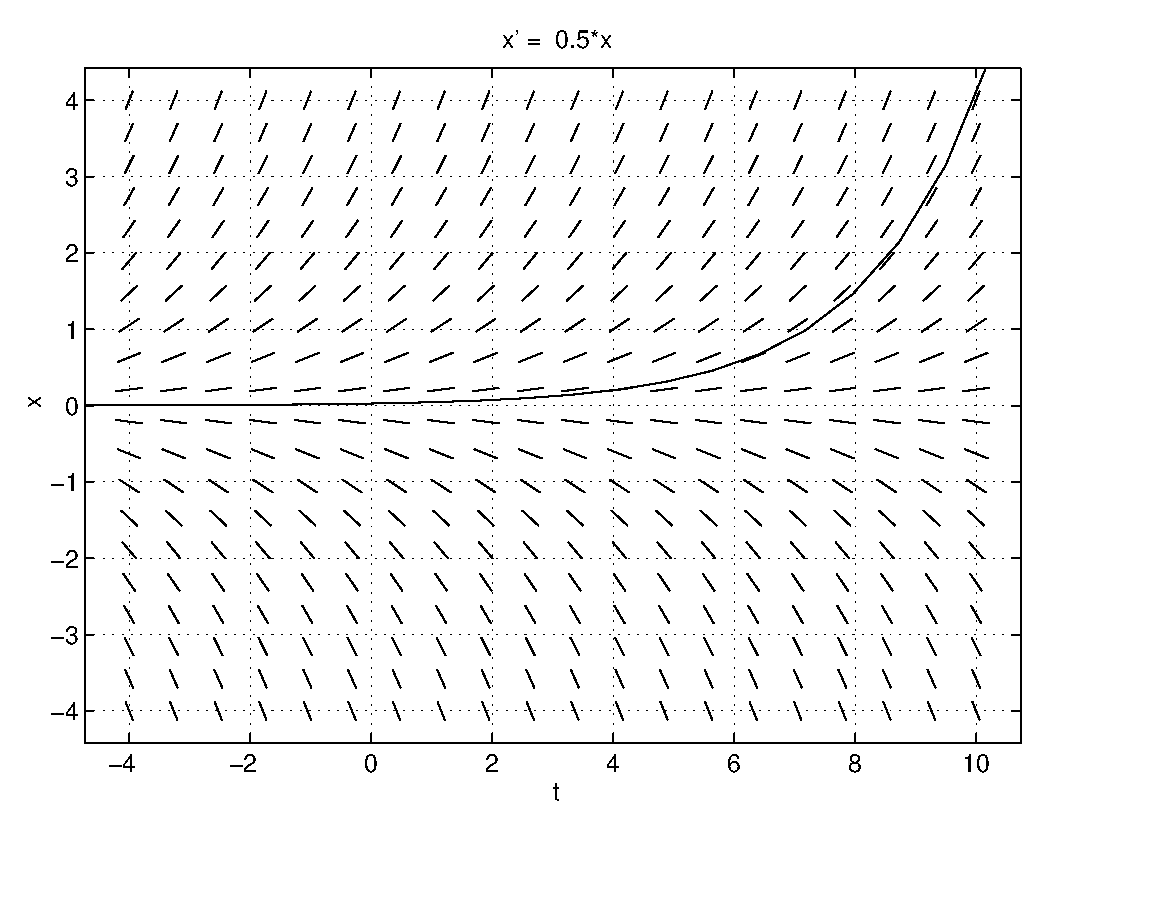
\psfig{file=figures/dfr_dsp1.eps,width=3.0in}}
    \caption{Left: Line field for $\dot{x}=0.5x$ for $t\in [-4,10]$ and
		$x\in [-4,4]$.  Right: A solution starting at $t=0$ and
		$x>0$ but small.}
    \label{df_dsp1}
\end{figure}

Now we may compute solutions going through a certain point
$(t_0,x_0)$ in the $(t,x)$-plane by clicking with any mouse
button on that point.  The solution is then computed first in
forward time and then in backward time.  For example, if we
click on a point near $t=x=0$ where $x>0$, {\sf dfield5} produces
the solution shown on the right in Figure~\ref{df_dsp1}.  Note
the similarity with the graph of the closed form solution in
Figure~\ref{graph_labelfig} when $\lambda=0.5$.

By clicking several times it appears that all solutions diverge
to either plus or minus infinity as $t$ goes to infinity.
Indeed, by \Ref{soln1} we know that the solutions are of the
form $x(t) = x_0 e^{0.5 t}$, and hence this behavior is expected
for $x_0\not= 0$.  To compute a solution corresponding to the case
when $x_0=0$, we bring up the menu {\sf DFIELD5 Options} and select
{\sf Keyboard input}.  This allows us to type in the initial
values $t=-2$ and $x=0$.  The action {\sf Compute} then leads to
the computation of the solution $x(t)=0$ corresponding to $x_0=0$.

The value of $\lambda=0.5$ can be changed by editing the
corresponding window in the {\sf DFIELD5 Setup.} For instance, if
we replace the $0.5$ by $-0.8$ and push {\sf Proceed}, then the
current line field is replaced by the line field shown
in Figure~\ref{df_dsp2}.
\begin{figure}[htb]
    \centerline{%
    \psfig{file=figures/df_dsp2.ps,width=3.0in}
    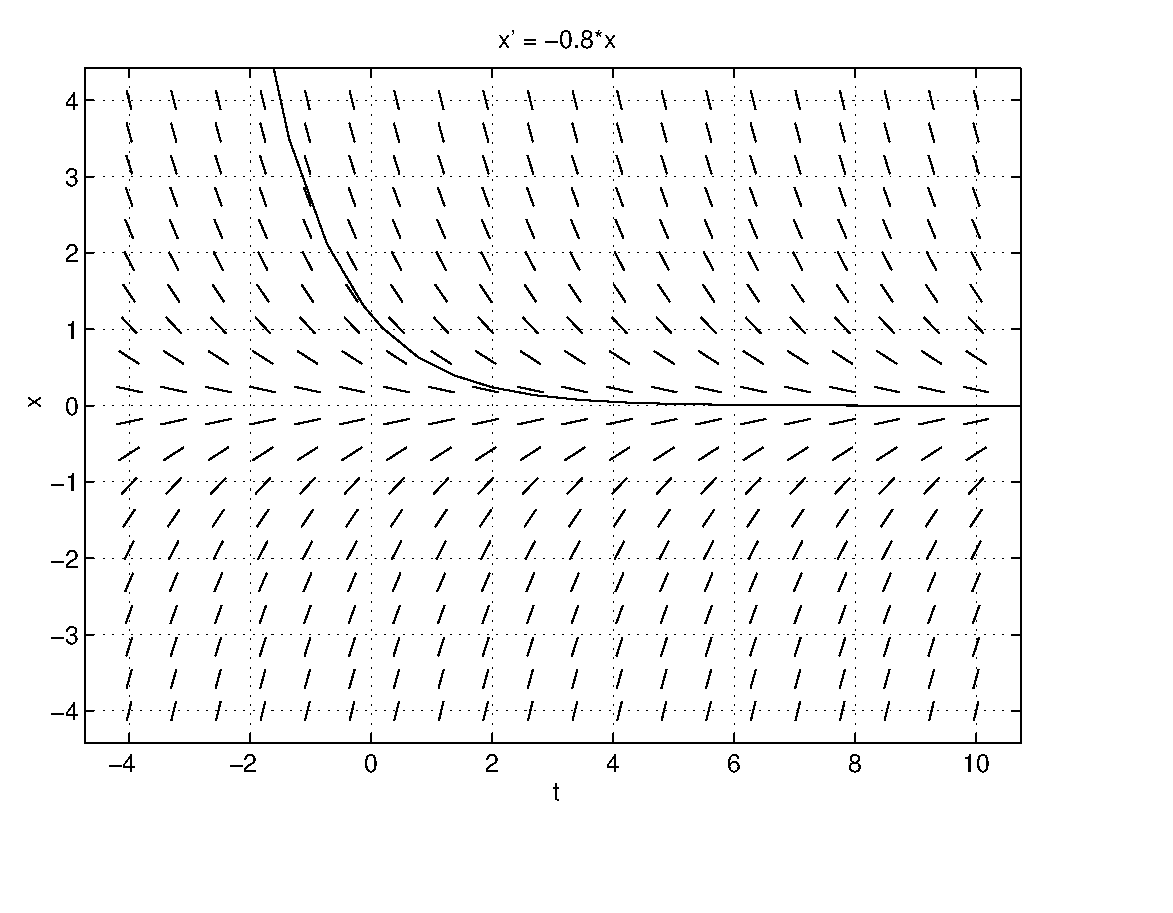
\psfig{file=figures/dfr_dsp2.eps,width=3.0in}}
    \caption{Left: Line field for $\dot{x}=-0.8 x$ for $t\in [-4,10]$
	and $x\in [-4,4]$.  Right: A solution starting at $t=0$ and
	$x$ between $1$ and $2$.}
    \label{df_dsp2}
\end{figure}

By computing different solutions, it seems as though all of them
converge to zero as $t$ goes to infinity, which agrees with
\Ref{explimits}.


\subsubsection*{Autonomous and Nonautonomous Equations in {\sf dfield5}}

In a sense, solutions of autonomous equations do not depend on the initial
time $t_0$, but just on the initial position $x_0$.  More precisely, let
$x_1(t)$ be the solution to
\[
\frac{dx}{dt} = f(x)
\]
with initial condition $x(0)=x_0$ and let $x_2(t)$ be a solution
to the same differential equation with initial condition $x(t_0)=x_0$.
Then
\begin{equation}  \label{E:initdiff}
x_2(t) = x_1(t-t_0).
\end{equation}
This statement can be verified by noting that the definition of
$x_2(t)$ in \Ref{E:initdiff} satisfies the initial value
\[
x_2(t_0)=x_1(t_0-t_0)=x_1(0)=x_0,
\]
and, using the chain rule, the differential equation
\[
\frac{dx_2}{dt}(t) = \frac{dx_1}{dt}(t-t_0) = f(x_1(t-t_0))=f(x_2(t)).
\]
So the solution $x_2(t)$ is the same as the solution $x_1(t)$ with
just a shift in time $t$.  In general, the same statement is {\em not\/} 
true for nonautonomous equations.

This difference between autonomous and nonautonomous equations can be
visualized using {\sf dfield5}. On the left in Figure~\ref{F:non-auto}
we graph two solutions of the {\em autonomous\/} differential equation
$\dot{x}=x^2-2x$ with initial conditions $x(0)=1$ and $x(2)=1$.  Note
that one solution is obtained from the other just by shifting by two
time units.  On the right of that figure we graph two solutions of the
{\em nonautonomous\/} differential equation $\dot{x}=x^2-t$ with
initial conditions $x(0)=1$ and $x(2)=1$.  Note that the two solutions
are most definitely not obtained one from the other by a time shift.

\begin{figure}[htb]
        \centerline{%
        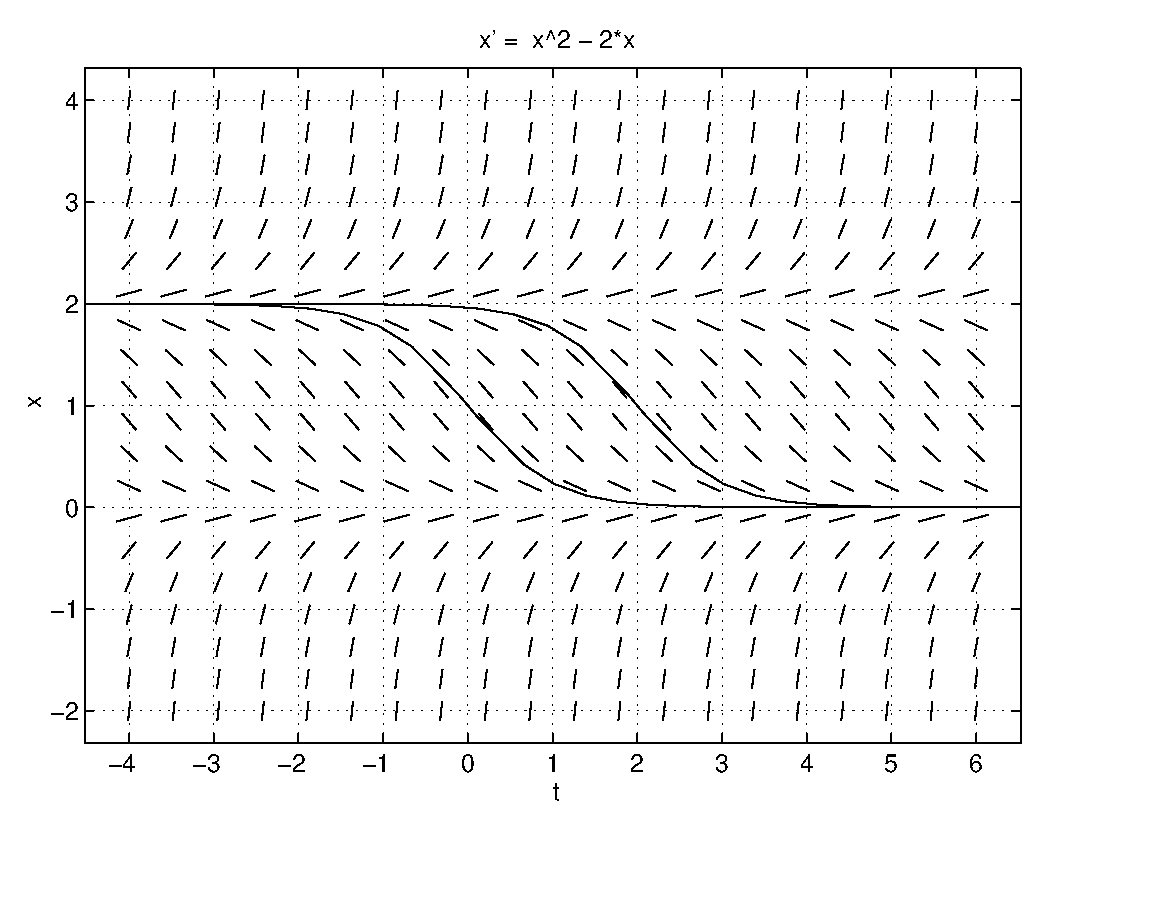
\psfig{file=figures/auto.eps,width=3.0in}
	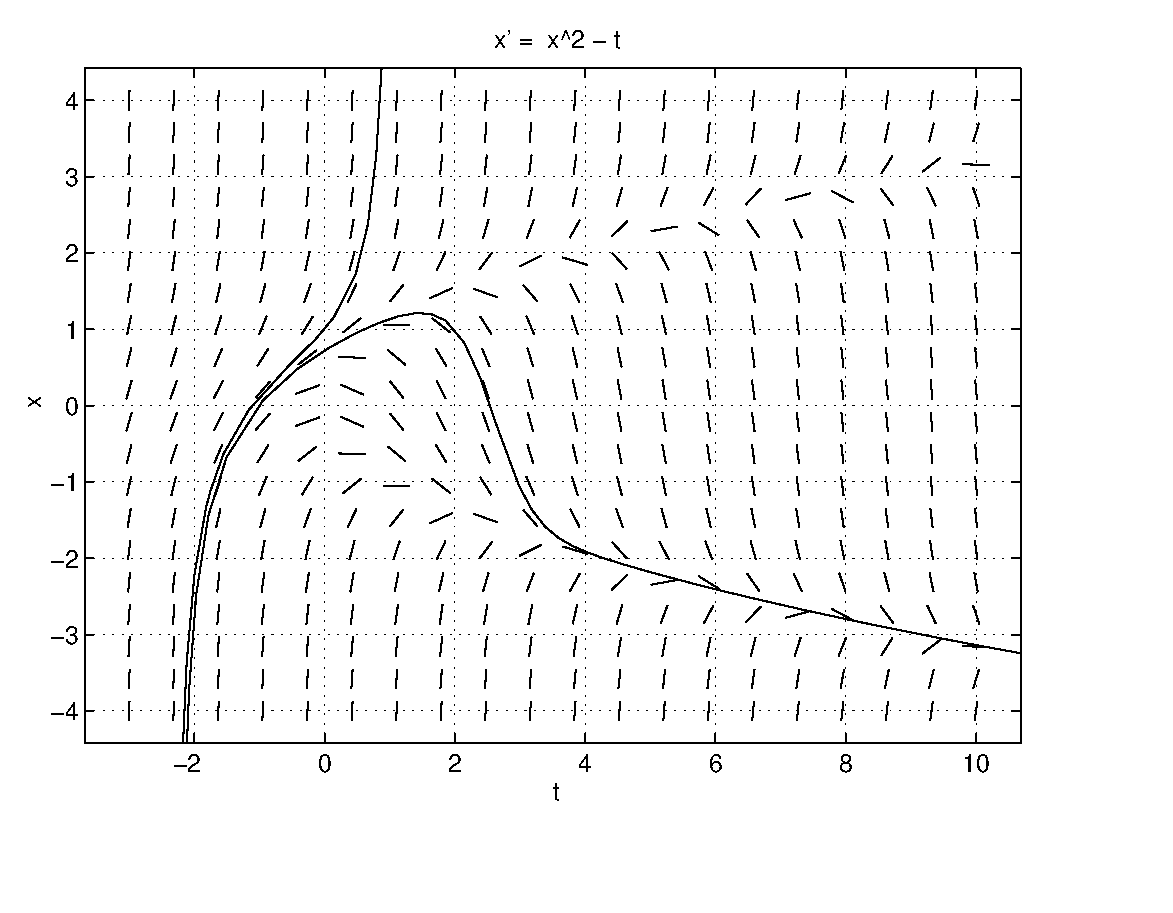
\psfig{file=figures/nonauto.eps,width=3.0in}}
        \caption{Left: Solutions of the autonomous equation $\dot{x}=x^2-2x$
	with initial conditions $x(0)=1$ and $x(2)=1$. Right: Solution of
	the nonautonomous differential equation $\dot{x}=x^2-t$ with initial
	conditions $x(0)=1$ and $x(2)=1$.}
        \label{F:non-auto}
\end{figure}


\EXER

\TEXER

\noindent In Exercises~\ref{c3.2.1A} -- \ref{c3.2.1D} determine whether the 
solution to the given differential equation with given initial condition is 
increasing or decreasing at the initial point.
\begin{exercise} \label{c3.2.1A}
ODE: $\dot{x}=x-t$; initial condition: $x(1)=2$.
\end{exercise}
\begin{exercise} \label{c3.2.1B}
ODE: $\dot{x}=x-t$; initial condition: $x(2)=1$.
\end{exercise}
\begin{exercise} \label{c3.2.1C}
ODE: $\dot{x}=x^2-tx$; initial condition: $x(1)=2$.
\end{exercise}
\begin{exercise} \label{c3.2.1D}
ODE: $\dot{x}=x^2-tx-t$; initial condition: $x(2)=-1$.
\end{exercise}

\noindent In Exercises~\ref{c3.2.2A} -- \ref{c3.2.2D} sketch by hand the line 
field of the given differential equation on the given rectangle.
\begin{exercise} \label{c3.2.2A}
ODE: $\dot{x}=x-t$; rectangle: $0\leq x\leq 2; -1\leq t\leq 1$.
\end{exercise}
\begin{exercise} \label{c3.2.2B}
ODE: $\dot{x}=x+t$; rectangle: $-2\leq x\leq 2; -1\leq t\leq 2$.
\end{exercise}
\begin{exercise} \label{c3.2.2C}
ODE: $\dot{x}=xt$; rectangle: $-1\leq x\leq 1; -1\leq t\leq 1$.
\end{exercise}
\begin{exercise} \label{c3.2.2D}
ODE: $\dot{x}=x/t$; rectangle: $0< x\leq 2; 0< t\leq 2$.
\end{exercise}

\noindent In Exercises~\ref{c3.2.3A} -- \ref{c3.2.3D} determine whether the 
given differential equation is autonomous or nonautonomous.
\begin{exercise} \label{c3.2.3A}
$\dot{x}=x-t$.
\end{exercise}
\begin{exercise} \label{c3.2.3B}
$\dot{x}=x^2-x$.
\end{exercise}
\begin{exercise} \label{c3.2.3C}
$\dot{x}=x\sin(x)$.
\end{exercise}
\begin{exercise} \label{c3.2.3D}
$\dot{x}=x\cos(t)$.
\end{exercise}


\CEXER

\noindent In Exercises~\ref{c3.2.a01a} -- \ref{c3.2.a01c} use
{\sf dfield5} to compute several solutions to the given differential
equations in the specified region.
\begin{exercise} \label{c3.2.a01a}
$\dot{x} = xt$, $t\in[0,2]$, $x\in[-1,1]$.
\end{exercise}
\begin{exercise} \label{c3.2.a01b}
$\dot{x} = tx^2$, $t\in[0,4]$, $x\in[-4,4]$.
\end{exercise}
\begin{exercise} \label{c3.2.a01c}
$\dot{x} = x-\sin(t)$, $t\in[-2,10]$, $x\in[-4,4]$.
\end{exercise}

\begin{exercise} \label{c3.2.1*}
Compute $x(2)$, where $x(t)$ is the solution to the differential equation 
$\dot{x} = 0.6x$ with initial condition $x(0)=0.5$, in two different ways, 
as follows:
\begin{itemize}
\item[(a)] Use {\sf Keyboard input} in {\sf dfield5} to compute the 
solution with initial value $x(0)=0.5$.  Use the {\sf zoom in} feature in 
the {\sf DFIELD5 Edit} menu to compute $x(2)$ to an accuracy of two decimal 
places.  (Drag a rectangle around the point you are interested in.  Repeat 
this several times until you can read off the value $x(2)$ of the solution.)  
\item[(b)] Use \Matlab to compute the value of the exact solution
of the form \Ref{soln1} with initial value $x(0)=0.5$.  
\item[(c)] Is your answer obtained using {\sf dfield5} in (a) accurate to 
within two decimal places of the answer obtained using (b)?  If not, 
which answer do you trust more, and why?
\end{itemize}
\end{exercise}

\begin{exercise} \label{c3.2.2}
Use {\sf dfield5} to compute solutions to the differential equation
$\dot{x} = x^2-tx+2t$. Use {\sf Keyboard input} to compute the solution
with initial value $x(-1)=-1$.  What is the minimum value of this
solution $x(t)$ on the interval $-2\leq t\leq 1$?  Plot
solutions to this equation starting with at least six or seven
different initial conditions. Then print the result.
\end{exercise}

\begin{exercise} \label{c3.2.3}
Use {\sf dfield5} to compute solutions to the differential
equation
\begin{equation}  \label{E:freehand}
\dot{x} = x^3-2t^2x-t.
\end{equation}
Print the line field of \Ref{E:freehand} on the intervals
$t\in[-2,2]$ and $x\in[-2,3]$.  Use the line field to draw freehand
the solution to \Ref{E:freehand} starting at $(t_0,x_0)=(-2,1)$.
Then set the initial condition using {\sf Keyboard input}
and print the numerically computed solution. Finally, compare
your freehand drawing with the numerically computed result.
\end{exercise}

\begin{exercise}  \label{exer:at}
\begin{itemize}
\item[(a)]  Draw the direction field for
\begin{equation} \label{ex:at}
\frac{dx}{dt} = \frac{x}{x-t}.
\end{equation}
Assuming that $x(2)=3$, estimate $x(137)$.
\item[(b)]  Verify that
\[
x(t) = t + \sqrt{t^2-3}
\]
is the solution to \Ref{ex:at}.  Then show that $x(t)$ satisfies the
initial condition $x(2)=3$.
\item[(c)]  Compare your estimate of the solution to \Ref{ex:at}
obtained using {\sf dfield5} with the exact solution
\[
x(137)= 137 +\sqrt{18766} \approx 273.989
\]
\end{itemize}
\end{exercise}

\Section{Phase Space Pictures and Equilibria} \label{S:PSP&E}

Recall that in a {\em phase space\/} \index{phase!space} plot, the 
solution $x(t)$ represents the position $x$ of a particle on a line 
for each time $t$.  Phase space plots are difficult to draw, since 
motion must be built into the plot.  However, we can view this 
dynamically in \Matlab using the program {\sf pline}. \index{\computer!pline}

In this discussion, we will only plot solutions of autonomous,
first order differential equations; that is, equations of the
form
\[
\dot{x} = g(x).
\]
To begin, type
\begin{verbatim}
pline
\end{verbatim}
and the window with the {\sf PLINE Setup} appears on the
computer screen.  The layout is essentially the same as in the
{\sf DFIELD5 Setup} described above.  However, there are two
differences:
\begin{enumerate}
\item Since we assume that our equation is autonomous, the time
variable --- the independent variable --- does
not appear explicitly and no time interval is specified.  Rather
the {\sf Integration time}, the period for which the solution is
to be computed, has to be declared.  This change is due to the
convention that all numerical computations start at $t=0$.
\item We may enter equations with one free parameter.
In the {\sf PLINE Setup} that parameter is {\sf lambda}.
Moreover, we may choose the value for that parameter.  The
default value in the {\sf PLINE Setup} is $-0.8$.  Hence, the
default equation used by {\sf pline} is equation
\Ref{lin1} with $\lambda = -0.8$.
\end{enumerate}

When we click with the left mouse button onto the button {\sf
Proceed}, then the display window with the title {\sf PLINE
Display} opens and the $x$-axis shown in Figure~\ref{pl_dsp1}
becomes visible.

\begin{figure}[htb]
     \centerline{%
     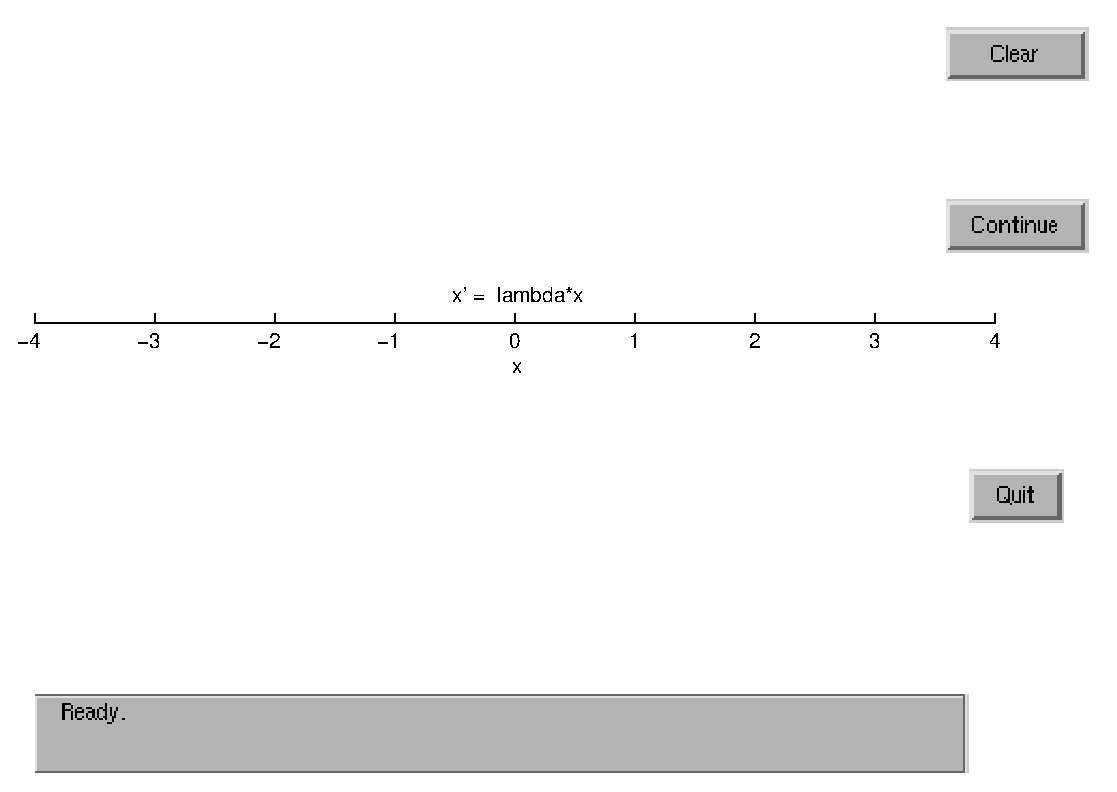
\psfig{file=figures/pl_dsp1.eps,height=2.6in}}
     \caption{{\sf PLINE Display} for $\dot{x}=\lambda x$
                and $x\in [-4,4]$.}
     \label{pl_dsp1}
\end{figure}

Similar to {\sf dfield5} we may start the numerical solution by
clicking with the left mouse button on the initial value of $x$.
It is not necessary to hit the axis precisely.  For example,
when we click (approximately) on $3$, a colored disk becomes
visible and moves to the left until it stops at a value for $x$
that is between $0.05$ and $0.06$.  This value can be read at
the bottom of the window from the message {\sf Endpoint:
0.05\ldots}.  We can also enter the initial point by choosing
the option {\sf Keyboard input} from the {\sf PLINE Options}
menu.  In fact, if we enter $x=3$ in that window and click on
{\sf Compute}, then the corresponding solution is computed and
we obtain the message {\sf Endpoint: 0.05495}.  Sometimes it
helps to clear all markers in the display window; this is
accomplished by clicking on {\sf Clear}.

\subsection*{Equilibria and Dynamics}

The simplest solution to a differential equation is a solution
that remains constant for all time.  Such solutions are called
{\em equilibria\/}.  Equilibria are found as follows:
\begin{lemma}  \label{L:equilibria}
Consider the autonomous \index{autonomous} differential equation
\begin{equation} \label{aut}
\frac{dx}{dt}(t) = g(x(t)).
\end{equation}
Then $x(t)=x_0$ is an equilibrium \index{equilibrium} if and only
if $g(x_0)=0$.
\end{lemma}

\proof Suppose that $x(t)=x_0$ is an equilibrium solution to
\Ref{aut}. Then $g(x_0)=0$, since $dx/dt = 0$.  Conversely,
suppose $g(x_0)=0$.  Then $x(t)=x_0$ is a solution to \Ref{aut}.
\qed

We now return to {\sf pline} and the autonomous equation
$g(x)=-0.8x$.  If we continue the integration by pushing {\sf
Continue} in the display window we see again that the solution
approaches $0$ as $t$ goes to infinity; that is, the solution
approaches the equilibrium given by $x(t)=0$.  Correspondingly,
the point that indicates the position of $x(t)$ in the display
window does not move any more.  Solutions that have initial
conditions near $0$ either tend towards $0$ when $\lambda <
0$ or away from $0$ when $\lambda> 0$.

An equilibrium $x(t)=x_0$ is {\em asymptotically stable\/}
\index{stability!asymptotic} if all solutions $y(t)$ with
initial condition $y(0)$ near $x_0$ have the limit
$x_0$ as $t$ goes to infinity.  In symbols we require
\[
\lim_{t\to\infty} y(t) = x_0.
\]
(The definition of asymptotic stability is more complicated in
higher dimensions.) The equilibrium $x(t)=x_0$ is {\em unstable\/}
\index{unstable} if trajectories starting near $x_0$ move away
from $x_0$.  Thus, in
our example, the equilibrium $x=0$ is {\em asymptotically
stable\/} when $\lambda< 0$ and {\em unstable\/}
when $\lambda> 0$.

The dynamical behavior of autonomous differential equations of
the form \Ref{aut} is essentially determined by the equilibria
of $g$.  We explore this statement by using {\sf pline} to
analyze the dynamical behavior of the ordinary differential
equation
\begin{equation} \label{pitch_eq}
	\dot{x} = x(\lambda-x^2),
\end{equation}
where $\lambda$ is a constant.  

First, enter this equation by editing the upper box in the 
{\sf PLINE Setup} window.  Do this editing by clicking in 
the window and deleting the default equation and then type 
{\sf x*(lambda-x\^{$\,\!$}2)}.  Then change the minimum 
and maximum values of $x$ from $-4$ and $4$ to $-2$ and $2$.  
Finally, change the integration time to $1$ and the value
of {\sf lambda} to $-1$.  

Second,  push on {\sf Proceed} so that the $x$ axis becomes 
visible in the display window.
On integrating the system, we find that solutions seem
to behave in a similar way to the solutions of \Ref{lin1} for
$\lambda < 0$: all the solutions approach zero as $t$ goes to
infinity.  Indeed, we can see that $x(t)=0$ is an equilibrium
solution of \Ref{pitch_eq} for all values of $\lambda$.  When
$\lambda<0$ numerical exploration suggests that $0$ is an
asymptotically stable equilibrium.

We now explore the stability properties of $x(t)=0$ when
$\lambda >0$.  We begin by changing the value of $\lambda$ to
$+1$.  We do this in the setup window and afterwards we confirm
the change by pushing {\sf Proceed}.  If we now compute
solutions of the differential equation, then we see that they
come to a rest at $+1$ if we start with a positive value for
$x(0)$ whereas they approach $-1$ if we start with a negative
value for $x(0)$.  Even if we begin the numerical computation
very close to $x=0$, the solutions tend to either $+1$ or $-1$.
These calculations indicate that $0$ is an unstable equilibrium
while both $+1$ and $-1$ are stable equilibria of \Ref{pitch_eq}
when $\lambda =1$.

We use the {\sf Keyboard input} to check that $x(t) = +1$ or
$x(t) = -1$ are equilibrium solutions.  Start the computations
with initial values $x(0) = +1$ or $x(0) = -1$ and see that the
solutions remain constant in time.  Alternatively, solve the
equation
\[
x(1-x^2) = 0,
\]
to see that $x=0,1,-1$ are all equilibria of \Ref{pitch_eq} when
$\lambda=1$.

Our numerical computations indicate that changing the
value of $\lambda$ from $-1$ to $+1$ changes the stability
property of the equilibrium $x(t)=0$.

We can now discuss a method for completely determining the
dynamics of a single autonomous differential equation \Ref{aut}
--- assuming that equilibria are isolated.

\begin{itemize}
\item Determine all equilibria of \Ref{aut} by solving the
equation $g(x)=0$.
\item Choose an initial point between each pair of consecutive
equilibria and determine the direction of motion (sign of $g$) at
that initial point. This can be done either directly or by using
{\sf pline}.
\item On a line plot the equilibria \index{equilibrium} and
connect them by arrows indicating the direction of the dynamics.
\end{itemize}
For example, the dynamics of the differential equations $\dot{x}
= x(-1-x^2)$ and $\dot{x} = x(1-x^2)$ are shown schematically in
Figure~\ref{pitch3}.

\begin{figure}[htb]
       \centerline{%
	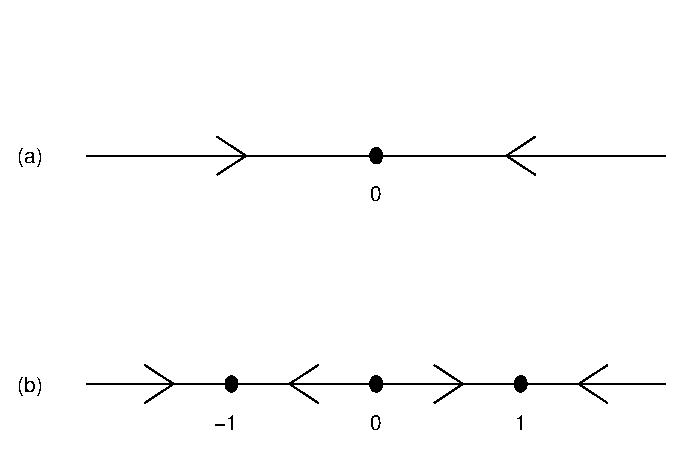
\psfig{file=figures/schemdyn.eps,width=3.4in}}
\caption{Schematic dynamics of (a) $\dot{x}=x(-1-x^2)$ and (b) $\dot{x}=x(1-x^2)$.}
\label{pitch3}
\end{figure}

\subsubsection*{Hyperbolic Equilibria}

Suppose that $x_0$ is an equilibrium for \Ref{aut}; that is suppose
$g(x_0)=0$.  We denote the derivative of $g(x)$ with respect to $x$, 
$dg/dx$, by $g'$.  The equilibrium $x_0$ is 
{\em hyperbolic\/} \index{hyperbolic}
if $g'(x_0)\neq 0$.  Assume that $x_0$ is a hyperbolic equilibrium and use
the tangent line approximation to $g(x)$ near $x_0$
($\Delta g = g'(x_0)\Delta x$) and that fact that $g(x_0)=0$ to conclude that
\[
g(x) \approx g'(x_0)(x-x_0).
\]
It follows that if $g'(x_0)<0$, then $g(x)$ is negative when
$x>x_0$ and positive when $x<x_0$.  So when $g'(x_0)<0$,
solutions of \Ref{aut} starting just to the right of $x_0$ will
move left ($g<0$) and tend towards $x_0$ and solutions starting
just to the left of $x_0$ will move right ($g>0$) and tend
towards $x_0$.  Similarly, if $g'(x_0)>0$, then $g(x)$ is positive
when $x>x_0$ and negative when $x<x_0$.  Thus, solutions near $x_0$ 
will tend away from $x_0$ when $g'(x_0)>0$.    We  have shown:
\begin{thm}[Stability of Hyperbolic Equilibria] \label{T:stability1}
Let $x_0$ be a hyperbolic equilibrium for the differential equation
\[
\frac{dx}{dt} = g(x).
\]
If $g'(x_0)<0$, then the equilibrium is asymptotically stable;
and if $g'(x_0)>0$, then the equilibrium is unstable.
\end{thm} \index{equilibrium} \index{stability!asymptotic}
\index{unstable}

It follows from Theorem~\ref{T:stability1} that the phase line picture
near a hyperbolic equilibrium is particularly simple as the arrows beside
that equilibrium either both point towards the equilibrium (as in
Figure~\ref{pitch3}(a)) or both point away from the equilibrium (as near $0$
in Figure~\ref{pitch3}(b)).

\subsection*{Comparing Phase Lines and Time Series}
\index{phase!line}\index{time series}

Phase line plots and time series graphs give different ways of
presenting the same information.  With that point in mind, it is
important to be able to recreate one type of plot from
the other.  For example, let $x(t)$ be the solution to the
differential equation $\dot{x}=x(1-x^2)$ with initial condition $x(0)=2$.
In Figure~\ref{pitch3}(b) we have drawn the schematic phase line for
all solutions to this differential equation. How can we reconstruct
a (schematic) graph of the time series $x(t)$ for this solution just
from the phase line?

To answer this question, note that in Figure~\ref{pitch3}(b) the
initial condition $x(0)=2$ lies to the right of all equilibria of
this equation, and the arrow indicates that solution trajectories
starting in this area move to the left, that is, they decrease to
the equilibrium at $x=1$.  It follows that
\[
\lim_{t\to\infty} x(t) = 1.
\]
Since there are no equilibria to the right of $x=2$, the graph of $x(t)$
must increase to infinity in {\em backwards\/} time.  So the graph of 
$x=x(t)$ is decreasing and asymptotic to $x=1$ for large positive $t$.  
A schematic graph is given in Figure~\ref{pitch3a}(a).  Using {\sf dfield5} 
we can check this description by numerically integrating the differential
equation.   This graph is shown in Figure~\ref{pitch3a}(b).

\begin{figure}[htb]
       \centerline{%
        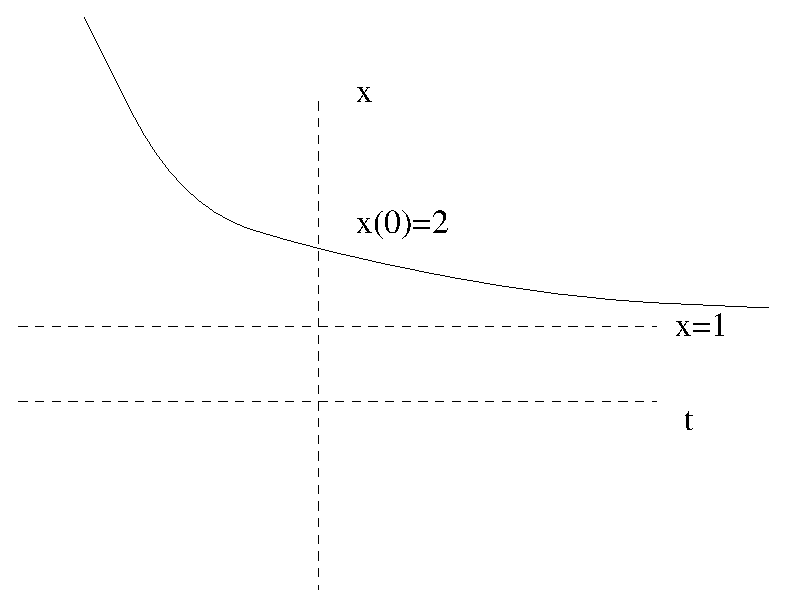
\psfig{file=figures/pitch3as.eps,width=2.8in}
	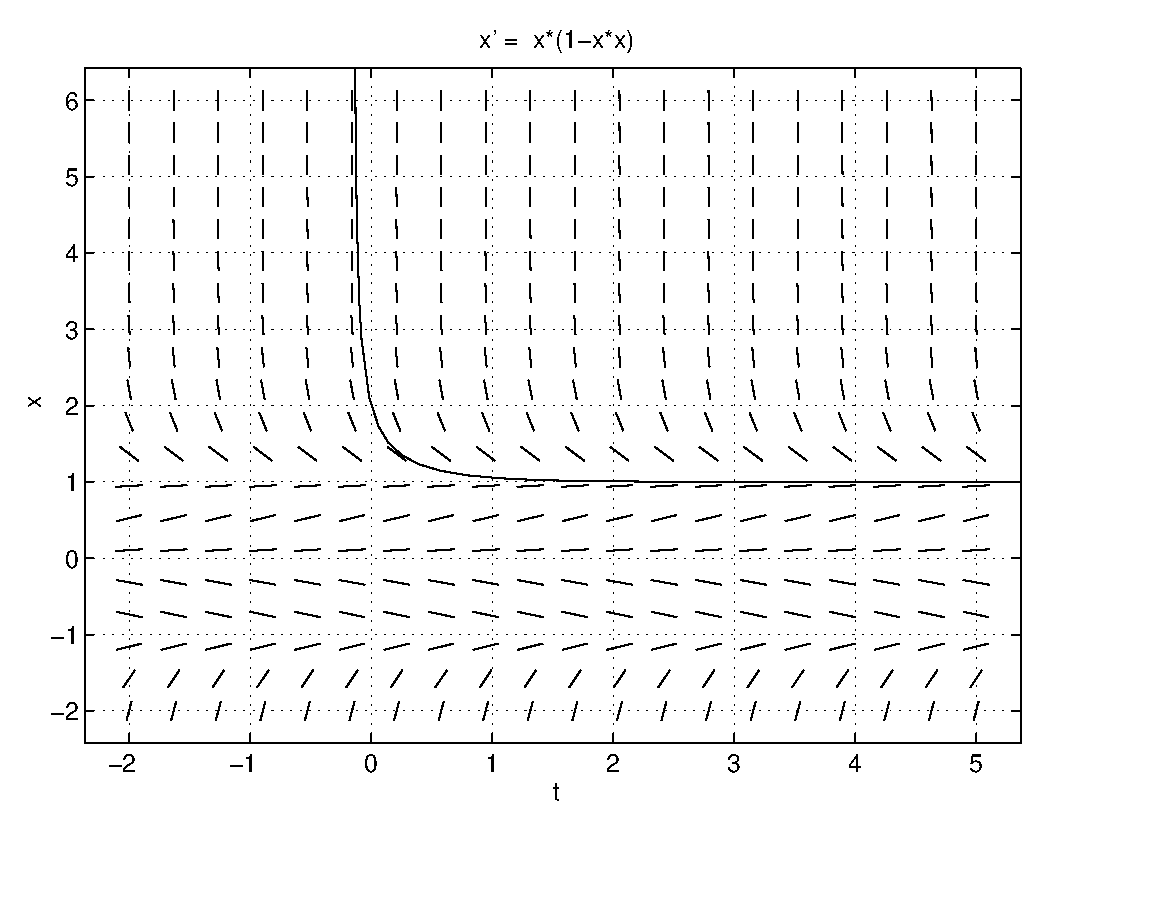
\psfig{file=figures/pitch3ad.eps,width=3.0in}}
       \caption{Time series for solution to $\dot{x}=x(1-x^2)$ with $x(0)=2$.
	(Left) Sketch using asymptotic information; (right) {\sf dfield5}
	computation.}
       \label{pitch3a}
\end{figure}



\EXER

\CEXER

\begin{exercise} \label{c3.3.1}
Use {\sf pline} to find an initial condition $x(0)$ for the
ordinary differential equation \Ref{lin1} with $\lambda=-0.2$
such that the corresponding solution $x(t)$ satisfies
$x(20)\in[0.001,0.002]$.
\end{exercise}

\begin{exercise} \label{c3.3.2}
Use {\sf pline} to find all the equilibria of the ordinary
differential equation
\[
\dot{x} = (x^2-1)(x+2).
\]
Which of the equilibria are stable and which are unstable?
\end{exercise}

\begin{exercise} \label{c3.3.3}
Consider the following ordinary differential equation:
\[
\dot{x} = \lambda x(1-x).
\]
Use {\sf pline} to find a value for the parameter $\lambda$ such
that $x(t)=1$ is a stable equilibrium.
\end{exercise}

\begin{exercise} \label{c3.3.4}
The differential equation
\[
\frac{dx}{dt} =  x^2
\]
has an equilibrium at the origin.  Use {\sf pline} to determine
those $x_0$ for which solutions to the initial value $x(0)=x_0$ tend
towards the origin.
\end{exercise}

\begin{exercise} \label{c3.3.5}
Consider the differential equation
\[
\frac{dx}{dt} = a x^3.
\]
Use {\sf pline} to verify that the origin is an asymptotically
stable equilibrium when $a = -1$ and is an unstable
equilibrium when $a = +1$. Discuss the relationship
between these examples and Theorem~\ref{T:stability1}.
\end{exercise}

\TEXER


\noindent In Exercises~\ref{c3.3.6A} -- \ref{c3.3.6D} compute the equilibria 
of the given differential equation, determine whether these equilibria are 
asymptotically stable or unstable, and draw a sche\-ma\-tic of the dynamics 
of this equation like the one in Figure~\ref{pitch3}.  You may use {\sf pline}
to check your answer.
\begin{exercise} \label{c3.3.6A}
$\dot{x} = x^2 + 2x - 3$.
\end{exercise}
\begin{exercise} \label{c3.3.6B}
$\dot{x} = x^3 - 2x^2 - 8x$.
\end{exercise}
\begin{exercise} \label{c3.3.6C}
$\dot{x} = x^3 + 2x^2 - 3x$.
\end{exercise}
\begin{exercise} \label{c3.3.6D}
$\dot{x} = x^2 + 6x + 1$.
\end{exercise}

\begin{exercise} \label{c3.3.7}
Let $x(t)$ be a solution to the initial value problem
\begin{eqnarray*}
\dot{x} & = & g(x) \\
x(0) & = & x_0.
\end{eqnarray*}
Let $y(t)=x(-t)$.  Show that $y(t)$ is a solution to the
initial value problem
\begin{eqnarray*}
\dot{y} & = & -g(y) \\
y(0) & = & x_0.
\end{eqnarray*}
(Thus, to integrate the solution $x(t)$ backwards in time is the
same as solving the differential equation $\dot{y}  =  -g(y)$
forward in time.)
\end{exercise}

\begin{exercise} \label{c3.3.9}
Use Exercise~\ref{c3.3.7} to devise a shortcut for solving
Exercise~\ref{c3.3.1}.
\end{exercise}

\begin{exercise} \label{c3.3.8}
Sketch the time series for the solution to the differential
equation pictured in Figure~\ref{pitch3}(b) with initial condition
$x(0)=\frac{1}{2}$.  Use only the phase space plot given in this
figure.  Use {\sf dfield5} to verify your answer.
\end{exercise}

\noindent In Exercises~\ref{c3.3.10a} -- \ref{c3.3.10d} use the line field 
given in Figure~\ref{F:exer3ad} to answer the following:\\
\noindent (a) Is the differential equation that was used to draw this figure 
autonomous or nonautonomous.\\
\noindent (b)  If the differential equation is autonomous, then draw the phase
line noting the values of $x$ where equilibria occur and whether they are 
asymptotically stable or not. If the differential equation is nonautonomous, 
then draw the time series for solutions with initial conditions $x(0)=0$ and 
$x(2)=0$.

\begin{exercise} \label{c3.3.10a}
Use Figure~\ref{F:exer3ad}(i) to answer parts (a) and (b).
\end{exercise}
\begin{exercise} \label{c3.3.10b}
Use Figure~\ref{F:exer3ad}(ii) to answer parts (a) and (b).
\end{exercise}
\begin{exercise} \label{c3.3.10c}
Use Figure~\ref{F:exer3ad}(iii) to answer parts (a) and (b).
\end{exercise}
\begin{exercise} \label{c3.3.10d}
Use Figure~\ref{F:exer3ad}(iv) to answer parts (a) and (b).
\end{exercise}

\begin{figure}[htb]
       \centerline{%
        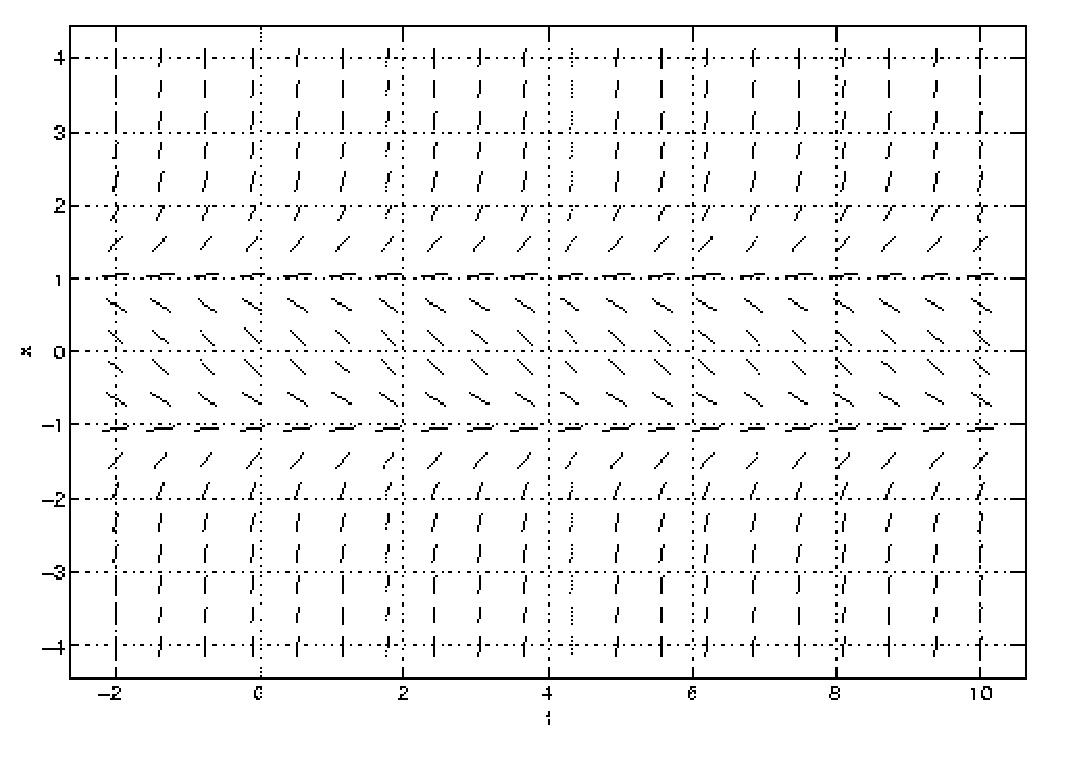
\psfig{file=figures/auto1a.eps,width=2.8in}
	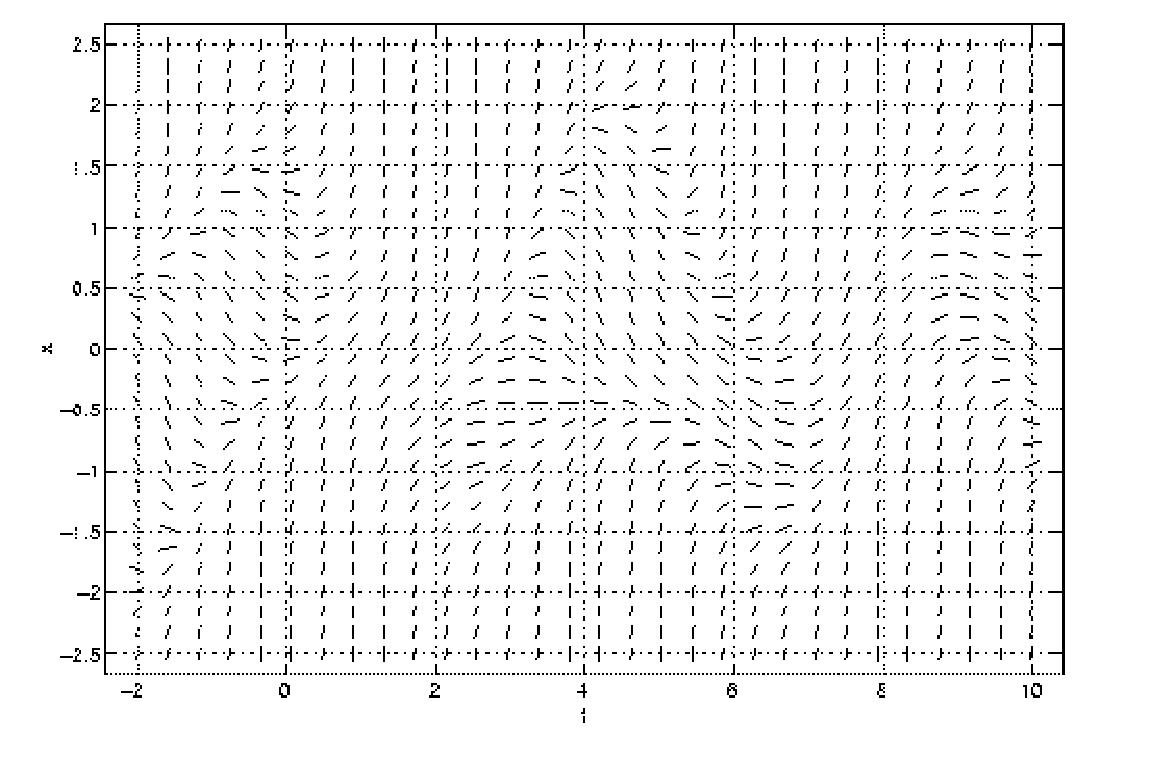
\psfig{file=figures/nonauto2a.eps,width=2.8in}}
\centerline{(i) \hspace{2.6in} (ii)}
       \centerline{%
        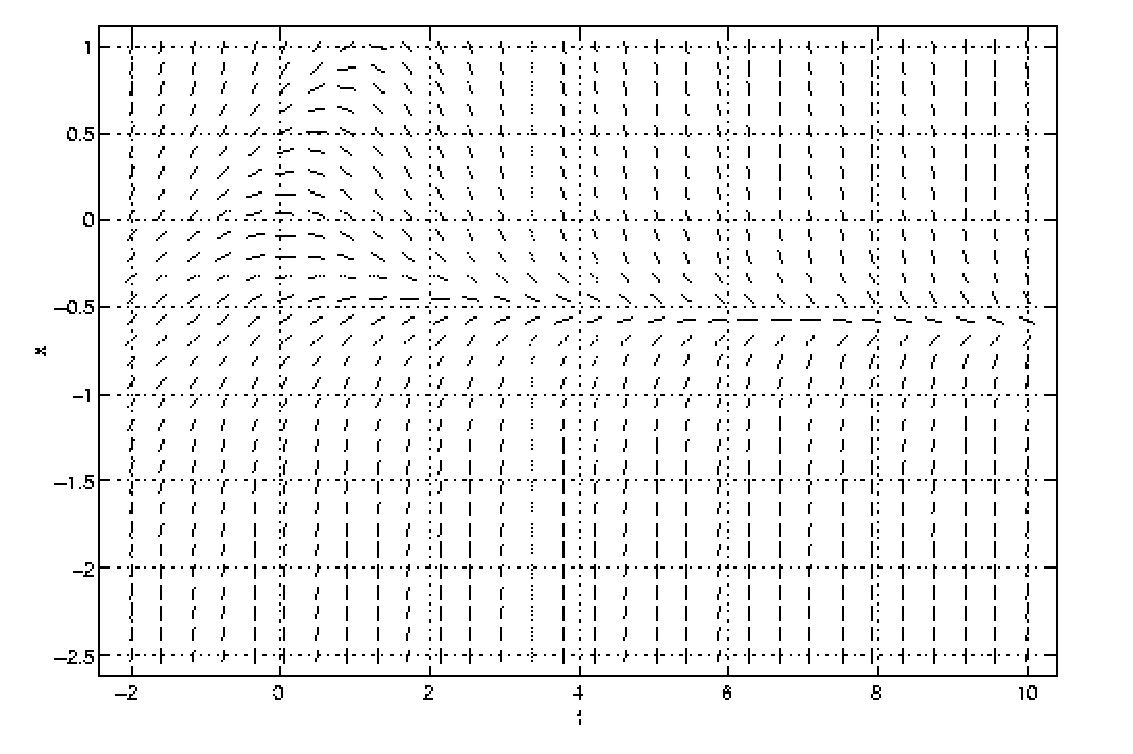
\psfig{file=figures/nonauto1a.eps,width=2.8in}
	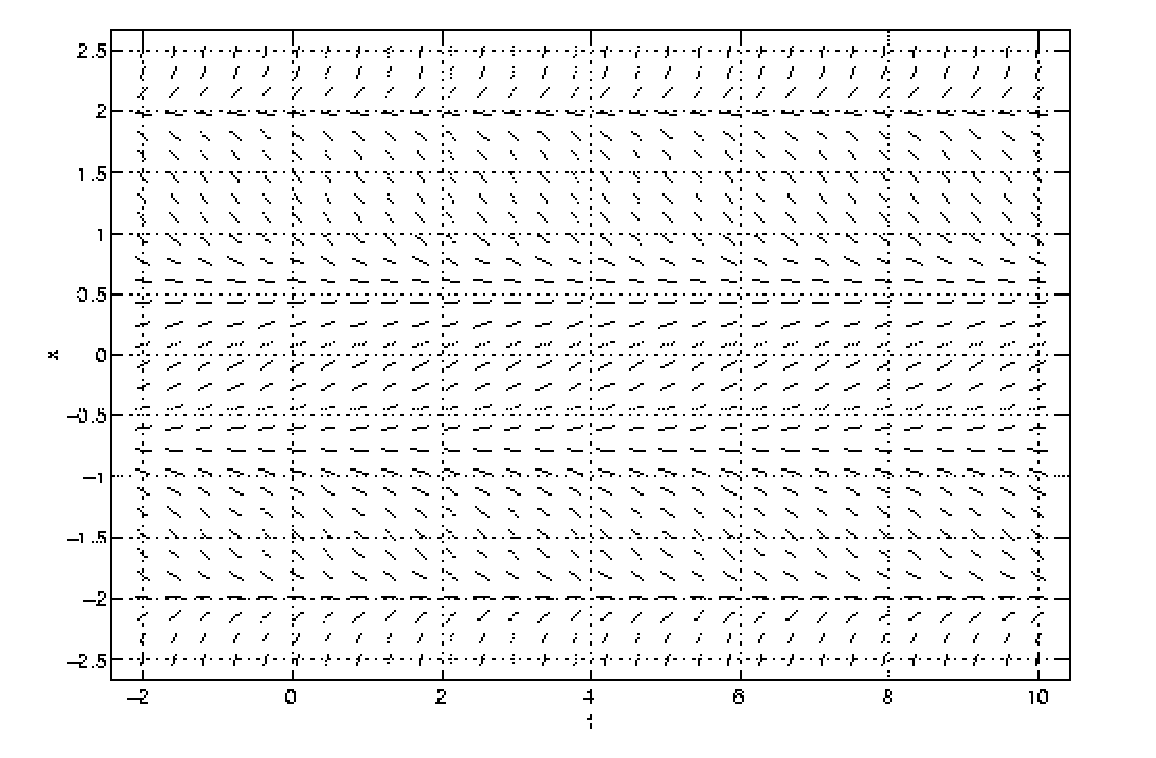
\psfig{file=figures/auto2a.eps,width=2.8in}}
\centerline{(iii) \hspace{2.6in} (iv)}
       \caption{Figures for Exercises~\protect{\ref{c3.3.10a}} --
\protect{\ref{c3.3.10d}}}
       \label{F:exer3ad}
\end{figure}


\Sec{*Separation of Variables}{SEPARATION OF VARIABLES}
\label{sec:sov} \index{separation of variables}

In this section we discuss a method for finding closed form solutions to
a particular class of nonautonomous first order ordinary differential 
equations\index{differential equation!first order} 
\begin{equation}  \label{e:nonauto}
\frac{dx}{dt} = f(t,x).
\end{equation}
These particular equations are {\em separable equations\/} having the form 
\begin{equation}  \label{eq:gh}
\frac{dx}{dt} = g(x) h(t),
\end{equation}
where $g,h:\R\to\R$ are continuous functions.   There are two special cases 
of \Ref{eq:gh}: the case $g(x)=1$ and the case $h(t)=1$.  

\subsubsection*{The Special Case $g(x)=1$: Integration Theory}

The assumption that $g(x)=1$ in \Ref{eq:gh} leads to the differential 
equation 
\begin{equation}  \label{e:g=1}
\frac{dx}{dt} = h(t).
\end{equation}
In Section~\ref{S:growthmodels} we saw that this differential equation  
is easily solved by direct integration.  For example, if $h(t)=t^2$ then 
the solution to \Ref{e:g=1} with initial condition $x(2)=5$ is found as
follows.  By direct integration,
\[
x(t) = \int t^2 dt = \frac{1}{3}t^3 + C.
\]
It then follows that
\[
x(2) = \frac{8}{3} + C = 5;
\]
so 
\[
C = 5 - \frac{8}{3} = \frac{7}{3}.
\]


\subsubsection*{The Special Case $h(t)=1$: Autonomous Equations}
\index{autonomous}

The second special case in \Ref{eq:gh} leads to the autonomous 
differential equation
\begin{equation}  \label{e:h=1}
\frac{dx}{dt} = g(x).
\end{equation}
Begin by noting that equilibria are special solutions to \Ref{e:h=1} that we 
can find by solving the equation $g(x)=0$.  More precisely, if $g(x_0)=0$, 
then $x(t)=x_0$ is a constant solution to \Ref{e:h=1}.  

We find the 
nonequilibrium solutions by direct integration --- but only after 
using change of variables in integration.  To solve \Ref{e:h=1},
just divide both sides of this equation by $g(x)$, obtaining
\[
\frac{1}{g(x)}\frac{dx}{dt} = 1,
\]
and integrate with respect to $t$, obtaining
\[
\int \frac{1}{g(x)} \frac{dx}{dt} dt = \int dt + C = t + C.
\]
After substituting $y=x(t)$ and using the chain rule, the integral on 
the left becomes
\[
\int\frac{1}{g(y)}dy.
\]
Replacing $y$ by $x$, we obtain
\[
\int\frac{1}{g(x)}dx = t + C.
\]

As a simple example, solve the growth rate equation \Ref{lin1} 
\begin{equation}  \label{lin1a} 
\frac{dx}{dt} = \lambda x
\end{equation}
using this technique of integration.  It follows that 
\[
\int \frac{1}{x}dx = \lambda t + C.
\]
So, to solve \Ref{lin1a}, we need to know how to integrate the function 
$1/x$.  Recalling that this integral is just $\ln |x|$ we obtain
\[
\ln |x(t)| = \lambda t + C.
\]
We solve this equation by exponentiation, obtaining
\[
|x(t)| = K e^{\lambda t},
\]
where $K = e^C \geq 0$.  On dropping the absolute value signs, we obtain
\[
x(t) =   K e^{\lambda t},
\]
for arbitrary $K$.  Of course, this is precisely the solution that we 
found in \Ref{soln1}.  

It is worth reflecting on the information from calculus that we needed to 
solve \Ref{lin1a}.  In Section~\ref{S:growthmodels} we found the solution to 
this equation by asking what function has a derivative that is a multiple of 
itself.  We then had to remember that $e^{\lambda t}$ is such a function and 
then prove that up to the constant $K$ this was the only such function 
(recall Theorem~\ref{T:singleeqn}).  Here we needed to remember the 
indefinite integral of $1/x$ and then solve for $x$ in terms of $t$.  

We now summarize this technique for solving the autonomous differential 
equation \Ref{e:h=1}.  Let $G(x)$ be an indefinite integral of $1/g(x)$. 
Then, after division by $g(x)$, integrating both sides of \Ref{e:h=1} 
with respect to $t$ leads to the equation 
\[
G(x) = t + C.
\]
Then we need to solve this algebraic equation for $x$ in terms of $t$.  This
last step is often quite difficult, as we show by example below.

There is one additional point that needs to be remembered when using 
this technique.  The constant $C$ is, as usual, related to an initial
condition.  Indeed, if we wish to solve \Ref{e:h=1} with the initial
condition $x(t_0)=x_0$, then we can solve for 
\[
C = G(x_0) - t_0.
\]

\subsubsection*{An Example of Blow-up in Finite Time}
\index{blow-up in finite time}

Consider the nonlinear differential equation
\begin{equation}  \label{e:x^2}
\frac{dx}{dt} = x^2
\end{equation}
satisfying the initial condition $x(t_0)=x_0$.  Using the preceding 
discussion, we can solve \Ref{e:x^2} by integration.  Specifically,
on division we obtain
\[
\frac{1}{x^2}\frac{dx}{dt} = 1,
\]
and on integration with respect to $t$, we obtain
\[
-\frac{1}{x} = t + C.
\]
Solving for $x$ in terms of $t$ we obtain
\[
x(t) = - \frac{1}{t+C}.
\]
Finally, use the initial condition to solve for $C$. On substitution 
\[
x_0 = x(t_0) = - \frac{1}{t_0+C}.
\]
Hence
\[
C = -\frac{1}{x_0} - t_0,
\]
which is fine unless $x_0$ happens to equal $0$.  However, in that case, we 
have just recovered the equilibrium solution $x(t)=0$.

On setting
\[
K = \frac{1}{x_0}+t_0,
\]
we obtain the solution
\[
x(t) =  \frac{1}{K-t}.
\]
For example, if $t_0=0.1$ and $x_0=2$, then $K=0.6$ and
\begin{equation} \label{E:solnx^2}
x(t) = \frac{1}{0.6-t}.
\end{equation}

Example~\Ref{e:x^2} shows that solutions to nonlinear differential
equations\index{differential equation!nonlinear} possess 
qualitative properties that are different from 
those of the linear equation $\dot{x}=\lambda x$.  In particular:
\begin{itemize}
\item Solutions can approach infinity in finite time.   For example, 
the solution \Ref{E:solnx^2} with initial condition $x(0.1)=2$ goes to 
infinity as $t$ approaches $0.6$.   
\item Solutions may not be defined for all $t\in\R$.  Indeed, the 
solution \Ref{E:solnx^2} has a singularity at $t=0.6$ and is defined 
for either $t> 0.6$ or $t<0.6$.  
\end{itemize}


We can solve equation \Ref{e:x^2} using 
{\sf dfield5}\index{\computer!dfield5}.
Using {\sf Keyboard input} set the initial condition at
$(x_0,t_0)=(2,0.1)$ and obtain the trajectory in
Figure~\ref{F:x^2}(left).  Note that this solution goes to infinity
in forward time while approaching $t=0.6$.  Now set the initial
condition to $(x_0,t_0)=(1,-2.5)$ and see that the solution goes
to negative infinity as $t$ approaches $0.6$ from above.  See
Figure~\ref{F:x^2}(right).  Finally note that both of these
solutions are given by the same formula \Ref{E:solnx^2}.

\begin{figure}[htb]
           \centerline{%
           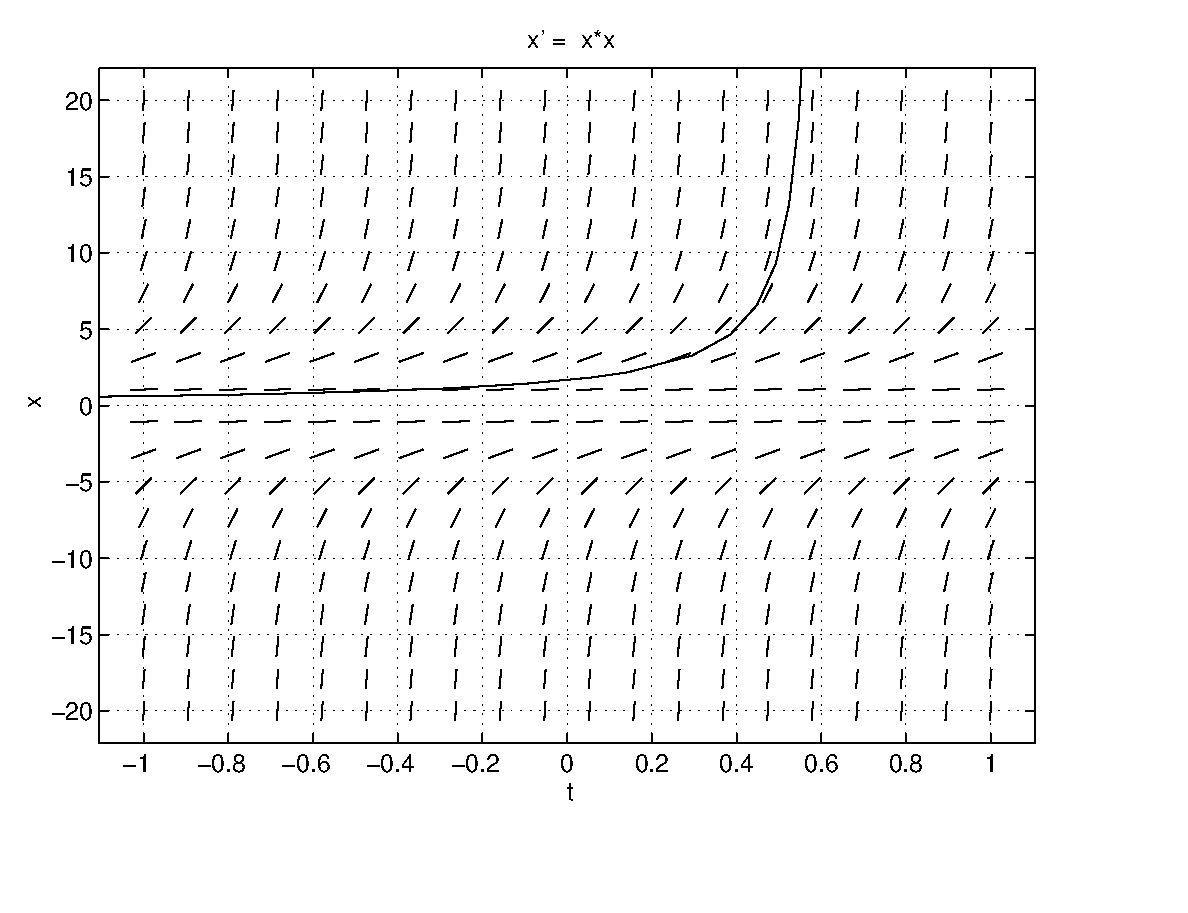
\psfig{file=figures/x2a.eps,width=3.5in}
	   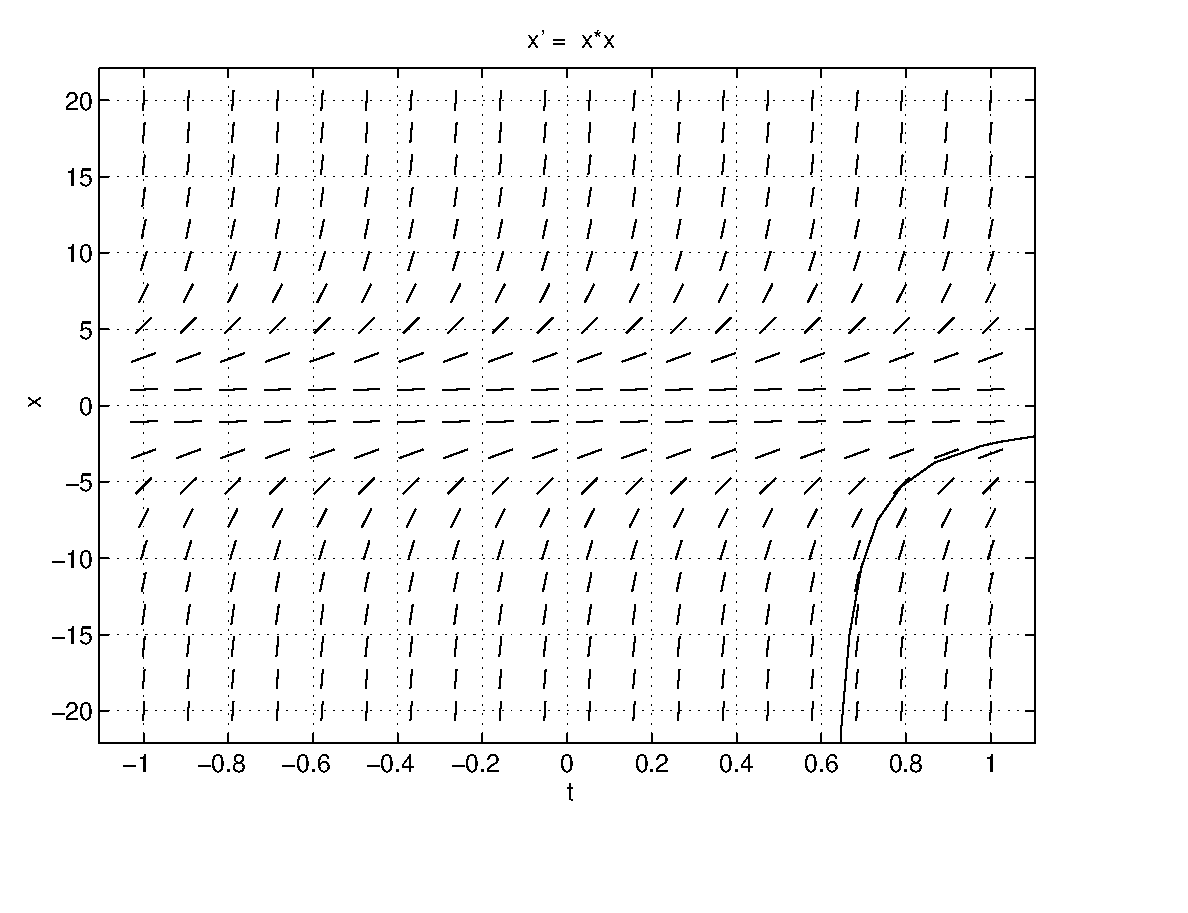
\psfig{file=figures/x2b.eps,width=3.5in}}
           \caption{Solutions using {\sf dfield5} for $\frac{dx}{dt} = x^2$ 
		with initial conditions: (left) $(x_0,t_0)=(2,0.1)$ and 
		(right) $(x_0,t_0)=(1,-2.5)$.}
           \label{F:x^2}
\end{figure}

\subsubsection*{An Example that Cannot be Solved in Closed Form}

Consider the differential equation
\begin{equation}  \label{E:ncf}
\frac{dx}{dt} = \frac{x}{x-1}
\end{equation}
with initial condition $x(1)=2$. On division \Ref{E:ncf} becomes 
\[
\left(1-\frac{1}{x}\right)\frac{dx}{dt} = 1.
\]
Integration with respect to $t$ yields
\[
x - \ln|x| = t + C.
\]
Using the initial condition, we see that 
\[
C = 2 - \ln 2 -1 = 1 - \ln 2.
\]
Note that for $t$ near $1$, the initial condition implies that $x(t)>0$.  
Hence $x(t)$ satisfies
\begin{equation} \label{e:solnncf}
x -\ln x = t + 1 - \ln 2.
\end{equation}
Unfortunately, this equation cannot be solved explicitly for $x$ 
as a function of $t$; that is, there is no closed form 
solution\index{closed form solution} 
for $x(t)$.  Nevertheless, $x(t)$ is defined 
{\em implicitly\/}\index{solution!implicitly defined} 
by \Ref{e:solnncf}.  This equation can, however, be solved numerically by
{\sf dfield5} just as easily as equations that have closed form solutions.
See Exercise~\ref{c14.1.17}. 

\subsection*{The General Solution by Separation of Variables}
\index{separation of variables!general solution}

The solution to the initial value problem for the separation
of variables equation
\begin{equation}  \label{eq:ghivp}
\dps \frac{dx}{dt} =  g(x) h(t),
\end{equation}
where $x(t_0) = x_0$, is obtained by combining the integrations of the two 
special cases just considered.  

Note that if $g(x_0)=0$, then $x(t)=x_0$ is an equilibrium solution to 
\Ref{eq:ghivp}.  So we can assume 
\begin{equation} \label{eq:gx0}
g(x_0)\not=0,
\end{equation}
and divide \Ref{eq:ghivp} by $g(x)$ to obtain
\[
\frac{1}{g(x)}\frac{dx}{dt}= h(t).
\]
Integrating with respect to $t$ yields
\[
\int \frac{1}{g(x)} \frac{dx}{dt}dt = \int h(t) dt + C.
\]
As before, on changing variables, we obtain
\[
\int\frac{1}{g(x)} dx = \int h(t) dt.
\]
Thus, the abstract solution to \Ref{eq:ghivp} can be written as
\begin{equation} \label{E:G=H+K}
G(x) = H(t) + C,
\end{equation}
where $G$ is an indefinite integral of $1/g$ and $H$ is an indefinite 
integral of $h$, and 
\begin{equation}  \label{E:G=H+Kinit}
C = G(x_0)-H(t_0).
\end{equation}



\subsubsection*{An Example Solving the Initial Value Problem}
\index{separation of variables!initial value problem}

We illustrate the technique of separation of variables with the following
example.  Find the solution of the initial value problem
\[
\frac{dx}{dt} = \frac{t}{x^2} 
\]
where $x(1)=2$.  Here $g(x) = 1/x^2$ and $h(t) = t$, so that
\[
G(x)=\int x^2 dx= \frac{1}{3}x^3 \AND H(t) = \int t dt = \frac{1}{2}t^2.
\]
Since $t_0=1$ and $x_0=2$, we can use \Ref{E:G=H+Kinit} to see that 
\[
C = G(2)-H(1) = \frac{8}{3} -\frac{1}{2} = \frac{13}{6},
\]
and \Ref{E:G=H+K} to see that the solution $x(t)$ satisfies
\[
\frac{1}{3}x(t)^3 = \frac{1}{2}t^2 + \frac{13}{6}.
\]
Therefore,
\[
x(t) = \left(\frac{3t^2+13}{2}\right)^{1/3}.
\]
The reader may check that this function is indeed a solution
satisfying the specified initial condition.

\subsubsection*{An Example Finding a General Solution}
\index{separation of variables!general solution}

With this example, we illustrate how to use separation of variables to find 
all solutions of a differential equation in the form \Ref{eq:gh}.  Consider
\begin{equation} \label{eq:x1t2}
\frac{dx}{dt} = \frac{(x+1)(t^2+1)}{t}
\end{equation}
for $t>0$.  Using our notation we have 
\[
g(x) = x+1 \AND h(t) = t+\frac{1}{t}.
\]
Note that $g(-1)=0$ and hence that $x(t)=-1$ is the constant equilibrium 
solution to \Ref{eq:x1t2}.  For all the other initial conditions, we obtain 
\[
G(x)=\int \frac{1}{x+1} dx = \ln|x+1| \AND 
H(t) = \int\left(t + \frac{1}{t}\right)dt = \frac{1}{2}t^2 + \ln |t|.
\]
Thus, in this example, identity \Ref{E:G=H+K} implies that the 
solution $x(t)$ satisfies
\[
\ln |x(t)+1| = \frac{1}{2}t^2 + \ln |t| + C.
\]
Hence
\[
|x(t)+1| = K|t|e^{t^2/2},
\]
for some constant $K>0$ and nonconstant solutions of \Ref{eq:x1t2} are in 
one-to-one correspondence with functions
\[
x(t) = Kte^{t^2/2}-1
\]
for $K\in\R$.  Note that setting $K=0$ recovers the constant solution 
$x(t)=-1$.

\EXER

\TEXER

\noindent In Exercises~\ref{c14.1.1a} -- \ref{c14.1.1d} decide whether 
or not the method of separation of variables can be applied to the given
differential equation.  If this method can be applied, then specify the 
functions $g$ and $h$ --- but do not perform the integrations.
\begin{exercise} \label{c14.1.1a}
$\dps \frac{dx}{dt} = x^{1/2}\cos t$.
\end{exercise}
\begin{exercise} \label{c14.1.1b}
$\dps \frac{dx}{dt} = (x+xt)\tan x$.
\end{exercise}
\begin{exercise} \label{c14.1.1c}
$\dps \frac{dx}{dt} = (x+t)(x-t)$.
\end{exercise}
\begin{exercise} \label{c14.1.1d}
$\dps \frac{dx}{dt} = 3-2x+3t-2xt$.
\end{exercise}

\noindent In Exercises~\ref{c14.1.5a} -- \ref{c14.1.5c} solve the given 
initial value problem by separation of variables. 
\begin{exercise}  \label{c14.1.5a}
$\dps \frac{dx}{dt} = -3x,\quad x(0)=-1.$
\end{exercise}
\begin{exercise}  \label{c14.1.5b}
$\dps \frac{dx}{dt} = \frac{t^3-1}{\cos x},
\quad x(\pi)=\frac{\pi}{2}.$
\end{exercise}
\begin{exercise}  \label{c14.1.5c}
$\dps \frac{dx}{dt} = 2\sqrt{tx},\quad x(1)=1.$
\end{exercise}

\noindent In Exercises~\ref{c14.1.8a} -- \ref{c14.1.8c} use separation 
of variables to find all the solutions of the given differential equation.
\begin{exercise}  \label{c14.1.8a}
$\dps \frac{dx}{dt} = 2x$.
\end{exercise}
\begin{exercise}  \label{c14.1.8b}
$\dps \frac{dx}{dt} = 5x+2$.
\end{exercise}
\begin{exercise}  \label{c14.1.8c}
$\dps \frac{dx}{dt} = \frac{\sin t}{x}$.
\end{exercise}

\CEXER

\noindent We have studied the autonomous linear differential equation 
$\dot{x}=\lambda x$ when $\lambda\neq 0$ and have shown that solutions 
exist for all time and tend either to $0$ or to $\pm\infty$ as $t\to\pm\infty$.
See \Ref{explimits} and Figure~\ref{df_dsp1}.  In Exercises~\ref{c14.1.11a} -- 
\ref{c14.1.11f} explore the behavior of solutions $x(t)$ of the given 
nonlinear (and often nonautonomous) differential equation using {\sf dfield5}.  
Where possible, describe the differences between the behavior of solutions of 
the given differential equation and the linear differential equation.  

\noindent{\bf Hint:}  Here is a list of properties of solutions that are 
{\em not valid\/} for solutions to the linear differential equation:
\begin{itemize}
\item[(a)]  Solutions blow up in finite time (that is, 
$\lim_{t\to t_0}x(t)=\pm\infty$).
\item[(b)]  Solutions do not exist for all time.
\item[(c)]  Multiple solutions are bounded in both forward and backward time.
(In the linear system only the zero solution $x(t)=0$ is bounded in both 
forward and backward time.)
\item[(d)]  Solutions stop (that is, solutions limit in either forward or 
backward time on a finite value of $x$ in finite time $t$).
\end{itemize}
Use {\sf dfield5} to determine which of these properties of solutions are 
valid for the given differential equations.  Also, when exploring 
Exercises~\ref{c14.1.11a} -- \ref{c14.1.11f} be prepared to use the {\sf Stop}
button in the {\sf DFIELD5 Display} window to stop the numerical integration. 

\begin{exercise} \label{c14.1.11a}
$\dps\frac{dx}{dt} = \frac{1}{x}$.
\end{exercise}
\begin{exercise} \label{c14.1.11b}
$\dps\frac{dx}{dt} = \frac{1}{tx}$.
\end{exercise}
\begin{exercise} \label{c14.1.11c}
$\dps\frac{dx}{dt} = \sin(tx)$.
\end{exercise}
\begin{exercise} \label{c14.1.11d}
$\dps\frac{dx}{dt} = t^2 - x^3$.
\end{exercise}
\begin{exercise} \label{c14.1.11e}
$\dps\frac{dx}{dt} = x(1-x^2)$.
\end{exercise}
\begin{exercise} \label{c14.1.11f}
$\dps\frac{dx}{dt} = \frac{t}{x^2}$.
\end{exercise}

\begin{exercise} \label{c14.1.17}
Recall that the differential equation \Ref{E:ncf} $\dot{x}=x/(x-1)$ cannot be 
solved in closed form.  
\begin{itemize}
\item[(a)]	Use {\sf dfield5}\index{\computer!dfield5} 
to solve this differential 
equation numerically on the interval $0.8\leq t\leq 1.2$ with initial 
condition $x(1)=2$.  (Set the $x$ interval to be $[0,4]$.)  
\item[(b)]	Using this result estimate the value of $x(1.15)$ to two 
decimal places.
\item[(c)]	Next change the time interval to be $0.5\leq t\leq 1.2$.
The numerically computed solution $x(t)$ behaves strangely when $t\leq 0.7$. 
What is the approximate value of $x$ in this range of $t$?  Use this 
observed value to explain why the numerical integration for this differential 
equation is badly behaved.
\end{itemize}
\end{exercise}

\begin{exercise} \label{c14.1.18}
The ability to find closed form solutions to differential equations enables
us to test the accuracy of numerically computed solutions.  As an example where difficulties arise in numerical computations, consider the differential 
equation
\begin{equation} \label{eq:exivp}
\frac{dx}{dt} = \left(\frac{x}{t}\right)^2.
\end{equation}
\begin{itemize}
\item[(a)] Use separation of variables to find the solution $x(t)$ to the 
initial value problem $x(0.001) = 2/1999$ of \Ref{eq:exivp}.
\item[(b)] Show that $\dps\lim_{t\to 2^-}x(t)=\infty$ for the solution of 
\Ref{eq:exivp} obtained in (a).
\item[(c)] For the initial condition specified in (a) compare the analytic 
solution of \Ref{eq:exivp} to the numerical solution computed by {\sf dfield5} 
in the region where the maximum value of $t$ is $2.5$ and the maximum value of 
$x$ is $100$.  How does the behavior of the numerically computed solution 
to \Ref{eq:exivp} differ from that of the analytically computed solution?
\item[(d)]  Compute the solution of \Ref{eq:exivp} using the general initial 
condition $x(t_0) = x_0$ where $t_0,x_0>0$ and show that 
$\lim_{t\to 0^+}x(t)=0$ for every such solution. 
\end{itemize}
\noindent {\bf Comment:} Part (d) hints at why there is a discrepancy 
between the numerically approximated solution and the analytic solution: 
small errors in the approximate solution with initial condition $(t_0,x_0)$ 
near $(0,0)$ cause different solutions to be computed.
\end{exercise}

 

\Section{Uncoupled Linear Systems of Two Equations}
\label{sec:UncoupledLS}

An autonomous system of two (first order) \index{first order}
differential equations \index{system of differential equations}
has the form
\renewcommand{\arraystretch}{1.8}
\begin{equation} \label{e:aut2}
\begin{array}{lll}
\dps \frac{dx}{dt}(t)  & = & f(x(t),y(t)) \\
\dps \frac{dy}{dt}(t)  & = & g(x(t),y(t)),
\end{array}
\end{equation}
where $f$ and $g$ are functions of the two variables $x$
and $y$.  Solutions to \Ref{e:aut2} are pairs of functions
$(x(t),y(t))$.

As in the single equation \Ref{aut}, the simplest
solutions are equilibria.  An {\em equilibrium\/} \index{equilibrium}
solution to
\Ref{e:aut2} is a solution where both functions $x(t)$
and $y(t)$ are constant functions; that is,
\[
x(t) = x_0 \AND  y(t)=y_0.
\]
For equilibria, it follows that both
\[
\frac{dx}{dt} = 0 \AND \frac{dy}{dt} = 0.
\]
Hence, equilibria of \Ref{e:aut2} can be found by
simultaneously solving the equations
\begin{eqnarray*}
f(x,y) & = & 0 \\
g(x,y) & = & 0.
\end{eqnarray*}

An autonomous {\em linear\/} system \index{linear!system} of ordinary
differential equations \index{system of differential equations!linear}
has the form
\renewcommand{\arraystretch}{1.8}
\begin{equation} \label{e:autlin}
\begin{array}{lll}
\dps \frac{dx}{dt}(t)  & = & a x(t) + b y(t) \\
\dps \frac{dy}{dt}(t)  & = & c x(t) + d y(t),
\end{array}
\end{equation}
\renewcommand{\arraystretch}{1.0}%
where $a,b,c,d$ are real constants.  Note that the origin
$(x(t),y(t))=(0,0)$ is always an equilibrium for a linear
system.

We begin our discussion of linear systems of ordinary
differential equations by considering uncoupled
\index{system of differential equations!uncoupled}systems of the form
\renewcommand{\arraystretch}{1.8}
\begin{equation} \label{lin2}
\begin{array}{lll}
\dps \frac{dx}{dt}(t) & = & a x(t) \\
\dps \frac{dy}{dt}(t) & = & d y(t).
\end{array}
\end{equation}
\renewcommand{\arraystretch}{1.0}%
Since the system is {\em uncoupled\/} (that is, the equation for
$\dot{x}$ does not depend on $y$ and the equation for $\dot{y}$
does not depend on $x$), we can solve this system by solving each
equation independently, as we did for \Ref{lin1}:
\begin{equation} \label{e:explicitsoln}
\begin{array}{ccc}
x(t) & = & x_0e^{at} \\
y(t) & = & y_0e^{dt}.
\end{array}
\end{equation}
There are now two initial conditions that are identified by
\[
x(0) = x_0 \AND y(0) = y_0.
\]

Having found all the solutions to \Ref{lin2} in \Ref{e:explicitsoln},
we now explore the geometry of the phase plane for
these uncoupled systems both analytically and by using \Matlabp.


\subsection*{Asymptotic Stability of the Origin}

As we did for the single equation \Ref{lin1}, we ask
what happens to solutions to \Ref{lin2} starting at $(x_0,y_0)$ as
time $t$ increases.  That is, we compute
\[
\lim_{t\to\infty}(x(t),y(t))=\lim_{t\to\infty}(x_0e^{a t},y_0e^{d t}).
\]
This limit is $(0,0)$ when both $a<0$ and $d<0$; but
if either $a$ or $d$ is positive, then most solutions diverge
to infinity, since either
\[
\lim_{t\to\infty}|x(t)| =\infty \quad \mbox{ or } \quad
\lim_{t\to\infty}|y(t)| =\infty.
\]


Roughly speaking, an equilibrium \index{equilibrium} $(x_0,y_0)$ is 
{\em asymptotically stable\/} \index{stability!asymptotic} if every 
trajectory $(x(t),y(t))$ beginning from an initial condition near 
$(x_0,y_0)$ stays near $(x_0,y_0)$ for all positive $t$, and
\[
\lim_{t\to\infty}(x(t),y(t)) = (x_0,y_0).
\]
The equilibrium is {\em unstable\/} \index{unstable} if there are  
trajectories with initial conditions arbitrarily close to the 
equilibrium that move far away from that equilibrium.

At this stage, it is not clear how to determine whether the
origin is asymptotically stable for a general linear system
\Ref{e:autlin}.  However, for uncoupled linear systems we
have shown that the origin is an asymptotically stable
equilibrium when both $a < 0$ and $d < 0$.  If either
$a >0$ or $d > 0$, then $(0,0)$ is unstable.

\subsubsection*{Invariance of the Axes}

There is another observation that we can make
for uncoupled systems.  Suppose that the initial condition for
an uncoupled system lies on the $x$-axis; that is, suppose $y_0=0$.
Then the solution $(x(t),y(t))=(x_0e^{at},0)$ also lies on the
$x$-axis for all time.  Similarly, if the initial condition lies
on the $y$-axis, then the solution $(0,y_0e^{dt})$ lies on the
$y$-axis for all time.

This invariance of the coordinate axes for uncoupled systems
follows directly from \Ref{e:explicitsoln}.  It turns out that
many linear systems of differential equations have invariant
lines; this is a topic to which we return later in this chapter.

\subsection*{Generating Phase Space Pictures with {\sf pplane5}}
\index{\computer!pplane5}

How can we visualize a solution $(x(t),y(t))$ to a system of
differential equations \Ref{e:aut2}?  The time series approach
suggests that we should graph $(x(t),y(t))$ as a function of $t$;
that is, we should plot the curve
\[
(t,x(t),y(t))
\]
in three dimensions.  Using \Matlab it is
possible to plot such a graph --- but such a graph by itself is
difficult to interpret.  Alternatively, we could graph either of
the functions $x(t)$ or $y(t)$ by themselves as we do for
solutions to single equations --- but then some information is
lost.

The method we prefer is the {\em phase space\/}\index{phase!space} 
plot obtained by thinking of $(x(t),y(t))$ as the
position of a particle in the $xy$-plane at time $t$.  We then
graph the point $(x(t),y(t))$ in the plane as $t$ varies.  When
looking at phase space plots, it is natural to call solutions
{\em trajectories\/},\index{trajectory} since we can imagine
that we are watching a particle moving in the plane as time
changes.

We begin by considering uncoupled linear equations.  As we saw,
when the initial conditions are on the coordinate axes (either
$(x_0,0)$ or $(0,y_0)$), the solutions remain on the coordinate
axes.  For these initial conditions, the equations behave as if
they were one dimensional.  However, if we consider an initial
condition $(x_0,y_0)$ that is not on a coordinate axis, then even
for an uncoupled system it is a little difficult to
{\em see\/} what the trajectory looks like.  At this point
it is useful to use the computer.

The method used to integrate planar systems of autonomous
differential equations is similar to that used to integrate
nonautonomous single equations in {\sf dfield5}.  The solution
curve $(x(t),y(t))$ to \Ref{e:aut2} at a point $(x_0,y_0)$ is
tangent to the direction $(f(x_0,y_0),g(x_0,y_0))$.  So
the differential equation solver plots the direction field
\index{direction field}
$(f,g)$ and then finds curves that are tangent to these
vectors at each point in time.

The program {\sf pplane5}\index{\computer!pplane5}, written by John
Polking,\index{Polking, John} is the two-dimensional analog of {\sf pline}.  
In \Matlab type
\begin{verbatim}
pplane5
\end{verbatim}
and the window with the {\sf PPLANE5 Setup} appears. {\sf pplane5}
has a number of preprogrammed differential equations listed in a
menu accessed by clicking on {\sf Gallery}.  To explore linear
systems, choose {\sf linear system} in the {\sf Gallery}.  (Note that the 
parameters in the {\sf linear system} are given by capitals rather than 
lower case {\sf a,b,c,d}.)

To integrate the uncoupled linear system, set the parameters $b$
and $c$ equal to zero. We now have the system \Ref{lin2} with
$a = 2$ and $d = -3$.  After pushing {\sf Proceed}, a display window
similar to {\sf dfield5} appears.  The main difference is that
the plane is filled by vectors $(f,g)$ indicating directions,
rather than by line segments indicating slopes.

As with {\sf dfield5} we may start the computations by clicking
with a mouse button on an initial value $(x_0,y_0)$.  For example,
if we click approximately onto $(x(0),y(0))=(x_0,y_0)=(1,1)$, then
the trajectory in the upper right quadrant of
Figure~\ref{pp_dsp1} displays.

\begin{figure}[htb]
     \centerline{%
     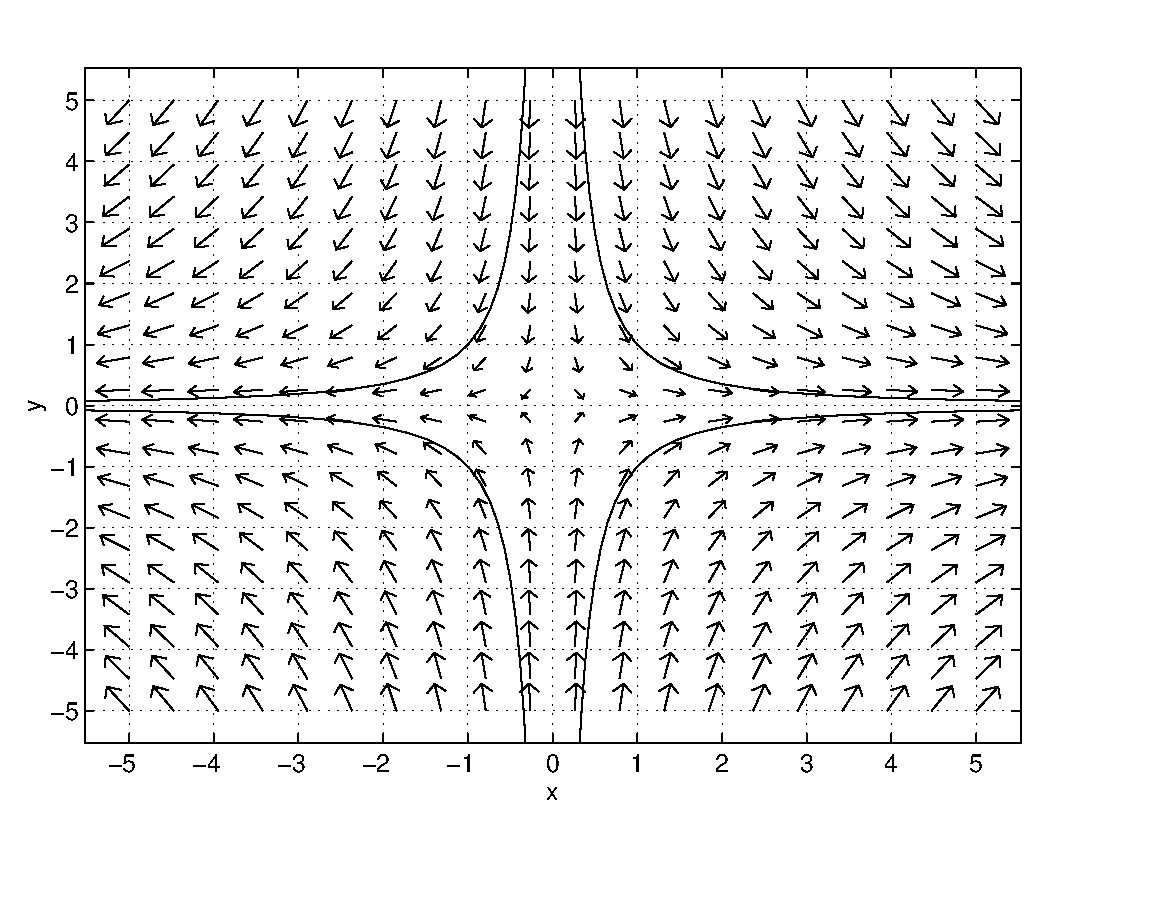
\psfig{file=figures/pp_dsp1.eps,width=3.5in}}
     \caption{{\sf PPLANE5 Display} for \protect\Ref{lin2} with
             $a=2$, $d=-3$ and $x,y\in [-5,5]$. Solutions
             going through $(\pm 1,\pm 1)$ are shown.}
     \label{pp_dsp1}
\end{figure}

First {\sf pplane5} draws the trajectory in forward time for
$t\ge 0$ and then it draws the trajectory in backwards time for
$t\le 0$.  More precisely, when we click on a point $(x_0,y_0)$ in
the $(x,y)$-plane, {\sf pplane5} computes that part of the
solution that lies inside the specified {\sf display window}
and that goes through this point.  For linear systems there is
precisely one solution that goes through a specified point in
the $(x,y)$-plane. We prove this fact in
Section~\ref{S:Matrixexp}.

\subsection*{Saddles, Sinks, and Sources for the Uncoupled System \protect{\Ref{lin2}}}

In a qualitative fashion, the trajectories of uncoupled linear
systems are determined by the invariance of the coordinate axes
and by the signs of the constants $a$ and $d$.

\subsubsection*{Saddles: $ad<0$} \index{saddle}

In Figure~\ref{pp_dsp1}, where $a=2>0$ and $d=-3<0$, the origin is a
{\em saddle\/}.  If we choose several initial values $(x_0,y_0)$
one after another,  then we find that as time increases all
solutions approach the $x$-axis.  That is, if $(x(t),y(t))$ is a 
solution to this system of differential equations, then 
$\lim_{t\to\infty}y(t)=0$.  This observation is particularly 
noticeable when we choose initial conditions close to the origin $(0,0)$.  
On the other hand, solutions also approach the $y$-axis as $t\to-\infty$.
These qualitative features of the phase plane are valid whenever 
$a>0$ and $d<0$.
 
When $a<0$ and $d>0$, then the origin is also a saddle ---
but the roles of the $x$ and $y$ axes are reversed.

\subsubsection*{Sinks: $a<0$ and $d<0$} \index{sink}

Now change the parameter $a$ to $-1$. After clicking on {\sf
Proceed} and specifying several initial conditions, we see that
all solutions approach the origin as time tends to infinity.
Hence --- as mentioned previously, and in contrast to saddles ---
the equilibrium $(0,0)$ is asymptotically stable.  Observe that
solutions approach the origin on trajectories that are tangent to
the $x$-axis.  Since $d<a<0$, the trajectory decreases to zero faster
in the $y$ direction than it does in the $x$-direction.  If
you change parameters so that $a<d<0$, then trajectories will
approach the origin tangent to the $y$-axis.

\subsubsection*{Sources: $a>0$ and $d>0$} \index{source}

Choose the constants $a$ and $d$ so that both are positive.
In forward time, all trajectories, except the equilibrium at the
origin, move towards infinity and the origin is called a
{\em source\/}.

\subsection*{Time Series Using {\sf pplane5}} \index{\computer!pplane5}

We may also use {\sf pplane5} to graph the time series of the
single components $x(t)$ and $y(t)$ of a solution $(x(t),y(t))$.
For this we choose {\sf x vs.\ t} from the {\sf Graph} menu.
After using the mouse to select a solution curve, another window
with the title {\sf PPLANE5 t-plot} appears.  There the time
series of $x(t)$ is shown.  For example, when the differential 
equation is a sink, we observe that this component
approaches $0$ as time $t$ tends to infinity.  We may also
display the time series of both components $x(t)$ and $y(t)$
simultaneously by clicking on {\sf Both} in the {\sf PPLANE5 t-plot} 
window.  Again we see that both $x(t)$ and $y(t)$ tend
to $0$ for increasing $t$.

We may also visualize the time series \index{time series} of
$x(t)$ and $y(t)$ in the three-dimensional $(x,y,t)$-space.  To
see this, click onto {\sf 3 D} and a curve $(x(t),y(t),t)$ 
becomes visible.  Since $x(t)$ and $y(t)$
approach $0$ for $t\to\infty$ we see that this curve
approaches the $t$-axis for increasing time $t$.  Finally, we
may look at all the different visualizations --- the phase space
plot, the time series for $x(t)$ and $y(t)$ and the
three-dimensional representation of the solution --- by clicking
the {\sf Composite} button.  See Figure~\ref{plotall}.


\begin{figure}[htb]
     \centerline{%
     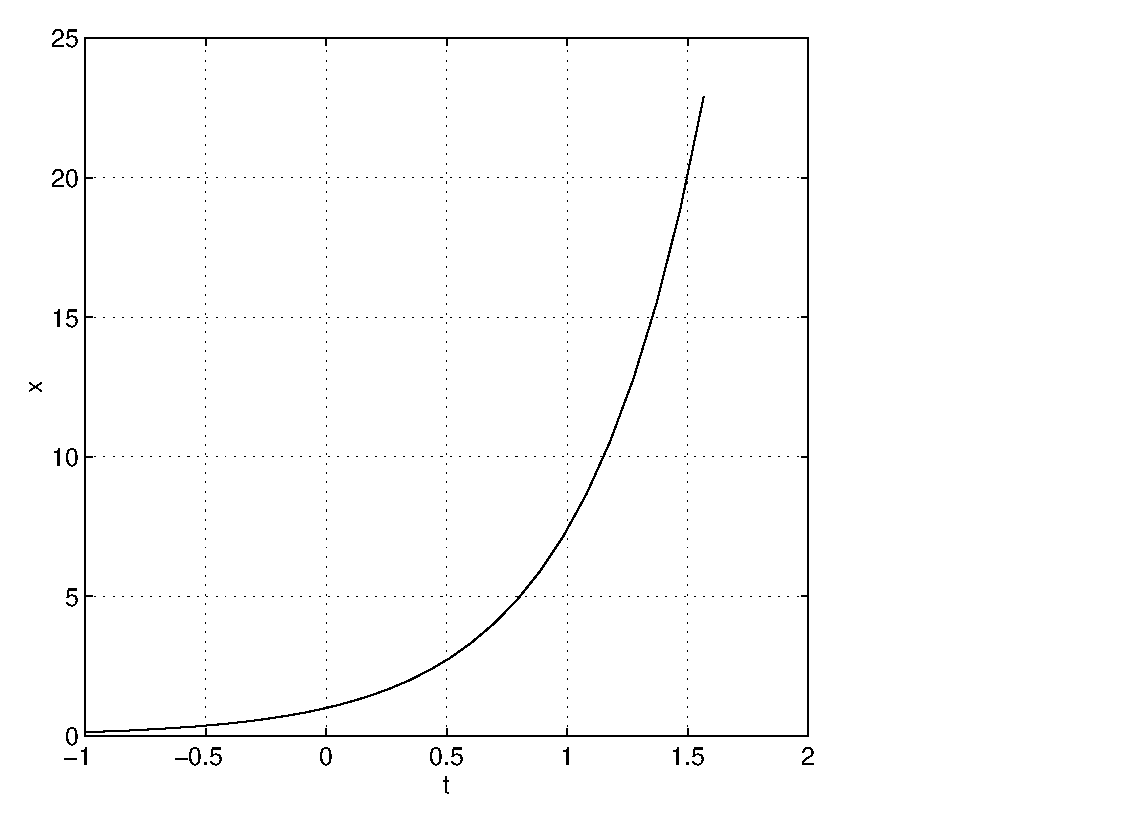
\psfig{file=figures/plotx.eps,height=2.0in,width=3.0in}
     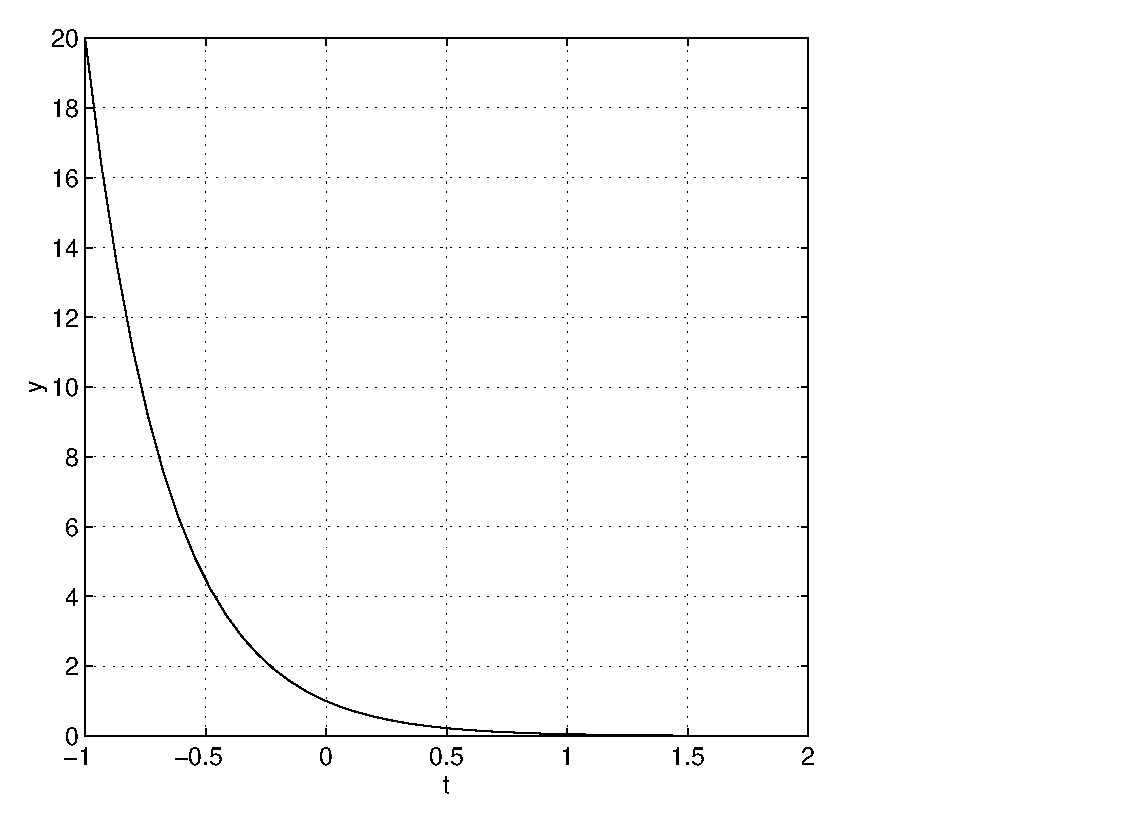
\psfig{file=figures/ploty.eps,height=2.0in,width=3.0in}}
     \centerline{%
     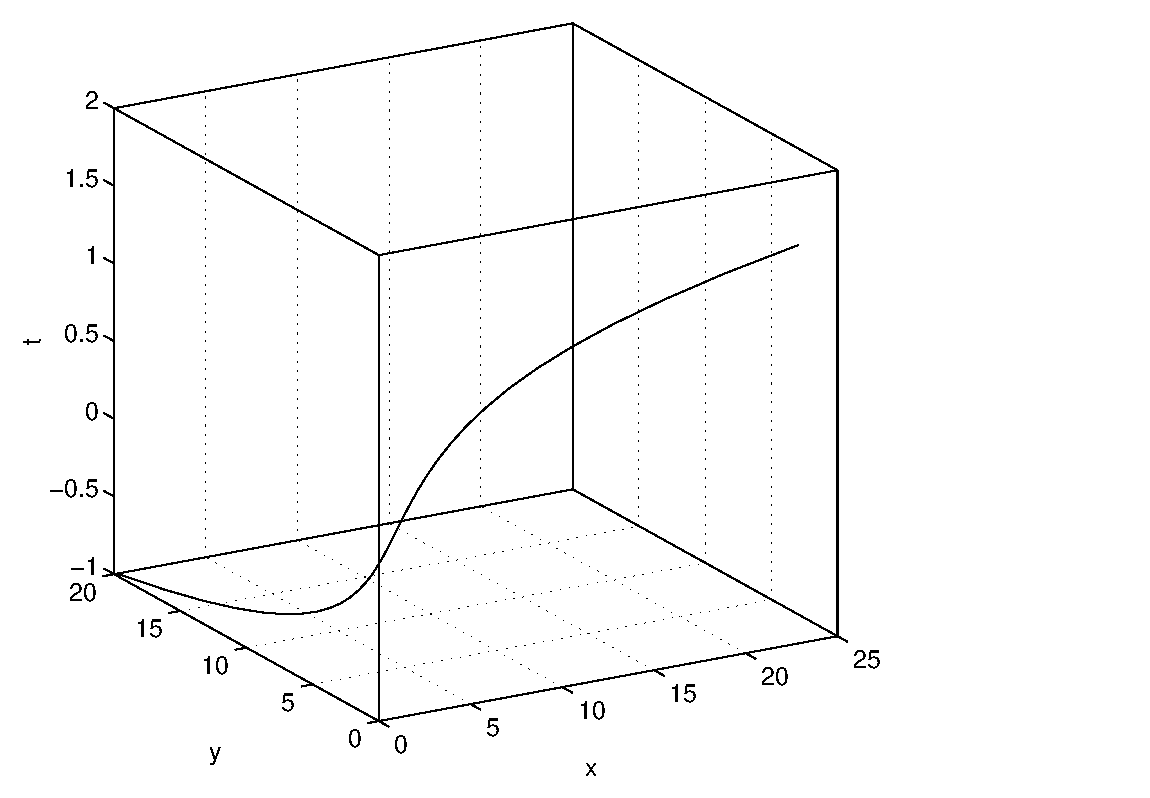
\psfig{file=figures/plot3d.eps,width=3.0in}
     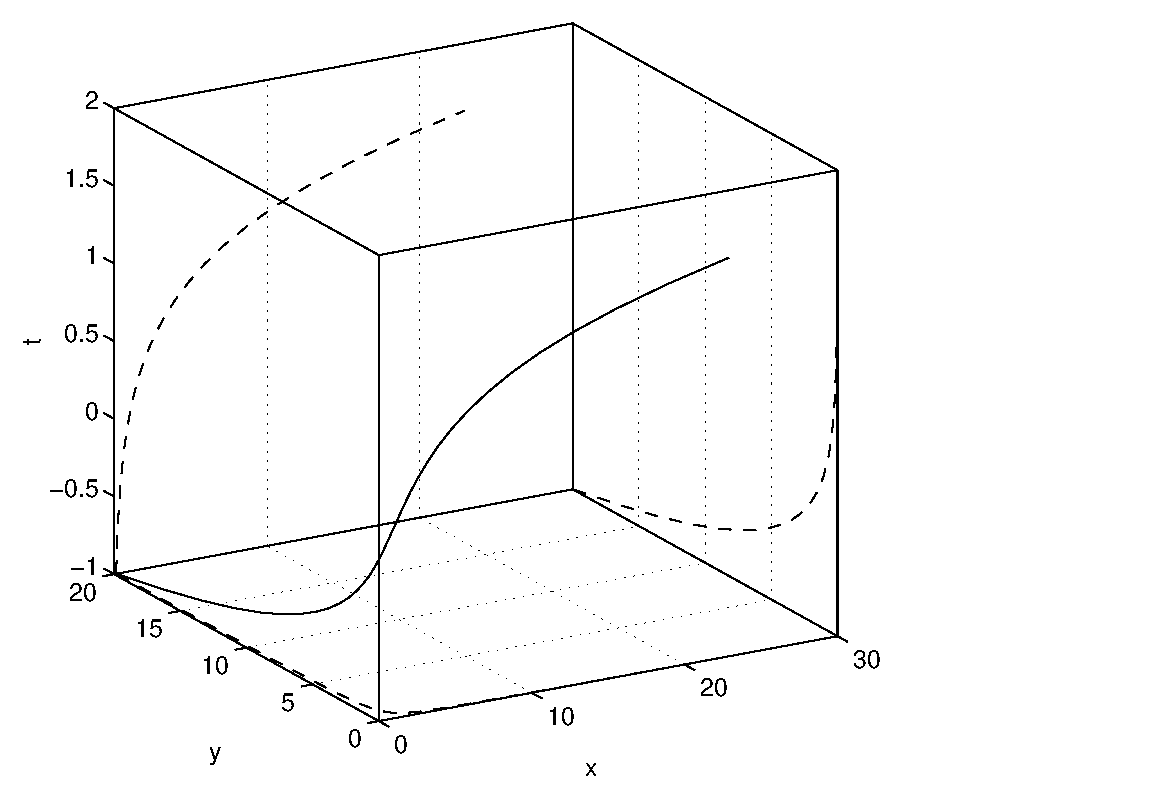
\psfig{file=figures/plotall.eps,width=3.0in}}
     \caption{{\sf PPLANE5 Display} for \protect\Ref{lin2} with
             $a=2$, $d=-3$ and $x\in [0,25], y\in [0,20]$. The solution
             going through $(1,1)$ is shown. UL: $(t,x(t))$;
	UR: $(t,y(t))$; LL: $(x(t),y(t),t)$; LR: all plots.}
     \label{plotall}
\end{figure}


\EXER

\TEXER

\noindent In Exercises~\ref{c3.5.1A} -- \ref{c3.5.1B} find all equilibria of
the given system of nonlinear autonomous differential equations.
\begin{exercise}  \label{c3.5.1A}
\begin{eqnarray*}
\dot{x} & = & x - y\\
\dot{y} & = & x^2 - y.
\end{eqnarray*}
\end{exercise}
\begin{exercise}  \label{c3.5.1B}
\begin{eqnarray*}
\dot{x} & = & x^2 - xy\\
\dot{y} & = & x^2 + y^2 - 4.
\end{eqnarray*}
\end{exercise}


\noindent In Exercises~\ref{E:uncoupleda} -- \ref{E:uncoupledc}
consider the uncoupled system of differential equations \Ref{lin2}.
For each choice of $a$ and $d$, determine whether the origin is a
saddle, source, or sink.
\begin{exercise} \label{E:uncoupleda}
$a=1$ and $d=-1$.
\end{exercise}
\begin{exercise} \label{E:uncoupledb}
$a=-0.01$ and $d=-2.4$.
\end{exercise}
\begin{exercise} \label{E:uncoupledc}
$a=0$ and $d=-2.3$.
\end{exercise}

\begin{exercise} \label{c3.4.2}
Let $(x(t),y(t))$ be the solution \Ref{e:explicitsoln} of \Ref{lin2}
with initial condition $(x(0),y(0))=(x_0,y_0)$, where $x_0\neq 0 \neq y_0$.
\begin{itemize}
\item[(a)] Show that the points $(x(t),y(t))$ lie on the curve whose 
equation is:
\[
y_0^ax^d - x_0^dy^a = 0.
\]
\item[(b)] Verify that if $a=1$ and $d=2$, then the solution lies
on a parabola tangent to the $x$-axis.
\end{itemize}
\end{exercise}

\begin{exercise} \label{c3.4.3}
Use the phase plane picture given in Figure~\ref{pp_dsp1} to
draw the time series $x(t)$ when $(x(0),y(0)) =
(\frac{1}{2},\frac{1}{2})$.  Check your answer using {\sf
pplane5}.
\end{exercise}

\CEXER


\begin{exercise} \label{c3.4.4}
For the three choices of $a$ and $d$ in the uncoupled system of
linear differential equations in Exercises~\ref{E:uncoupleda} -- 
\ref{E:uncoupledc}, use {\sf pplane5}
to compute phase portraits.  Use {\sf Keyboard input} to look at
solutions with initial conditions on the $x$ and $y$ axes.  As time
$t$ increases, do solutions with these initial conditions tend towards 
or away from the origin?
\end{exercise}

\begin{exercise} \label{c3.4.5}
Suppose that $a$ and $d$ are both negative, so that the origin
is asymptotically stable.  Make several choices of $a<d<0$ and
observe that solution trajectories tend to approach the origin
tangent to one of the axes.  Determine which one.  Try to prove
that your experimental guess is always correct?
\end{exercise}

\begin{exercise} \label{c3.4.6}
Suppose that $a=d<0$.  Verify experimentally using {\sf pplane5}
that all trajectories approach the origin along straight lines.
Try to prove this conjecture?
\end{exercise}

\begin{exercise} \label{c3.4.7}
Use {\sf pplane5} to compute several solutions of the linear system by
setting $a=2$ and $d=-3$ in the region $x,y\in[-5,5]$.  Then use
{\sf dfield5} to compute several solutions of the single differential
equation
\[
\frac{dx}{dt} = -\frac{2x}{3t}
\]
for $x,t\in[-5,5]$.  Is there a relationship between solutions to the
two equations and can you explain what that relationship is?
\end{exercise}



\Section{Coupled Linear Systems} \index{coupled system} \label{s:3.5}


The general linear constant coefficient system in two unknown functions 
$x_1,x_2$ is:
\renewcommand{\arraystretch}{1.8}
\begin{equation}\label{lin3}
\begin{array}{ccc}
\dps \frac{dx_1}{dt}(t) & = & ax_1(t) + bx_2(t) \\
\dps \frac{dx_2}{dt}(t) & = & cx_1(t) + dx_2(t).
\end{array}
\end{equation}
\renewcommand{\arraystretch}{1.0}%
The uncoupled systems studied in Section~\ref{sec:UncoupledLS} are obtained 
by setting $b=c=0$ in \Ref{lin3}.  We have discussed how to solve \Ref{lin3} 
by formula \Ref{e:explicitsoln} when the system is uncoupled.  We have also 
discussed how to visualize the phase plane for different choices of the 
diagonal entries $a$ and $d$.  At present, we cannot
solve \Ref{lin3} by formula when the coefficient matrix is not diagonal.
But we may use {\sf pplane5} to solve the initial value problems numerically 
for these coupled systems.  We illustrate this point by solving
\begin{eqnarray*}
\frac{dx_1}{dt}(t) & = &  -x_1(t) + 3x_2(t) \\
\frac{dx_2}{dt}(t) & = &  3x_1(t) - x_2(t).
\end{eqnarray*}
After starting {\sf pplane5}, select {\sf linear system} from the
{\sf Gallery} and set the constants to:
\[
	a = -1,\quad b = 3,\quad c = 3, \quad d = -1.
\]
Click on {\sf Proceed}.  In order to have equally spaced coordinates on
the $x$ and $y$ axes, do the following.   In the {\sf PPLANE5 Display} 
window click on the {\sf edit} button and then on the {\sf zoom in square} 
command.  Then, using the mouse, click on the origin.

\subsection*{Eigendirections}

After computing several solutions, we find that for increasing
time $t$ all the solutions seem to approach the diagonal line
given by the equation $x_1=x_2$. Similarly, in backward time $t$
the solutions approach the anti-diagonal $x_1=-x_2$.  In other
words, as for the case of uncoupled systems, we find two
distinguished directions in the $(x,y)$-plane.  See
Figure~\ref{F:invariantlines}.  Moreover, the computations
indicate that these lines are invariant in the sense that
solutions starting on these lines remain on them for all time.
This statement can be verified numerically by using the {\sf
Keyboard input} in the {\sf PPLANE5 Options} to choose initial
conditions $(x_0,y_0)=(1,1)$ and $(x_0,y_0)=(1,-1)$.

\begin{figure}[htb]
     \centerline{%
     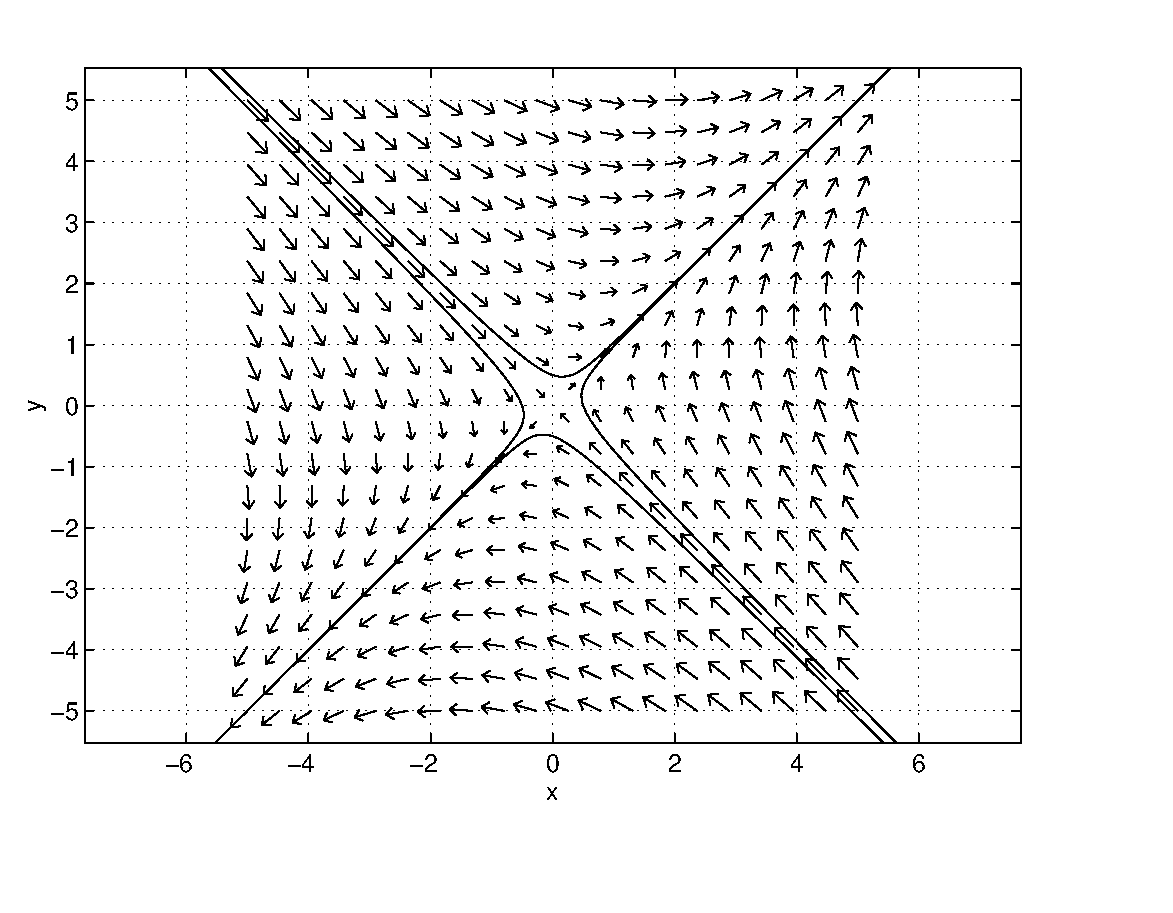
\psfig{file=figures/invline.eps,width=3.5in}}
     \caption{{\sf PPLANE5 Display} for \protect\Ref{lin3} with
             $a=-1=d$; $b=3=c$; and $x,y\in [-5,5]$.
	Solutions going through $(\pm 0.5,0)$ and $(0,\pm 0.5)$ are shown.}
     \label{F:invariantlines}
\end{figure}

\begin{Def} \label{D:eigendirection}
An invariant line for a linear system of differential equations
is called an {\em eigendirection}\index{eigendirection}.
\end{Def}

Observe that eigendirections vary if we change parameters.  For
example, if we set $b$ to $1$, then there are still two
distinguished lines but these lines are no longer perpendicular.

For uncoupled systems, we have shown analytically that the $x$
and $y$ axes are eigendirections.  The numerical computations
that we have just performed indicate that eigendirections exist
for many coupled systems.  This discussion leads naturally to
two questions:
\begin{enumerate}
\item Do eigendirections always exist?
\item How can we find eigendirections?
\end{enumerate}
The second question will be answered in Sections~\ref{S:IVP&E} and 
\ref{S:evchp}.  We can answer the first question by performing another 
numerical computation.  In the setup window, change the parameter $b$ 
to $-2$.  Then numerically compute some solutions to see that there
are no eigendirections in the phase space of this system.  Observe that
all solutions appear to spiral into the origin as time goes to
infinity.  The phase portrait is shown in Figure~\ref{pp_dsp2}.
\begin{figure}[htb]
      \centerline{%
      \psfig{file=figures/pp_dsp2.ps,width=3.5in}}
      \caption{{\sf PPLANE5 Display} for the {\sf linear system}
		with $a=-1$, $b=-2$, $c=3$, $d=-1$.}
      \label{pp_dsp2}
\end{figure}

\subsubsection*{Second Order Differential Equations}
\index{differential equation!second order}

We now show analytically that certain linear systems of
differential equations have no invariant lines in their phase portrait.

We do this by showing that second order differential equations can be
reduced to first order systems by a simple but important trick.  Indeed,
sometimes it is easier to solve a single second order equation, and
sometimes it is easier to solve the first order system.  At this stage
we introduce this connection by considering the differential equation
\begin{equation}  \label{E:2ndordera}
\frac{d^2x}{dt^2} + x = 0.
\end{equation}
This differential equation states that we are looking for a function
$x(t)$ whose second derivative is $-x(t)$.  From calculus, we know
that $x(t)=\cos t$ is such a function.

Let $y(t)=\dot{x}(t)$.  Then
\Ref{E:2ndordera} may be rewritten as a first order coupled system
in $x(t)$ and $y(t)$ as follows:
\begin{equation}  \label{E:2nd->1st}
\begin{array}{rcl}
\dot{x} & = & y \\
\dot{y} & = & -x.
\end{array}
\end{equation}
Observe that if $x(t)$ is a solution to \Ref{E:2ndordera}, then
\[
0 = \frac{d^2x}{dt^2} + x = \frac{dy}{dt} + x.
\]
Hence,
\[
\dot{y} = -x
\]
Conversely, if $(x(t),y(t))$ is a solution to \Ref{E:2nd->1st}, then
$x(t)$ is a solution to \Ref{E:2ndordera}.  That is,
\[
\frac{d^2x}{dt^2} + x = \frac{dy}{dt} + x = -x + x = 0.
\]

It follows from the discussion that $(x(t),y(t))=(\cos t,\sin t)$ is 
a solution to the differential equation \Ref{E:2nd->1st}.  We have shown 
analytically that the unit circle centered at the origin is a solution 
trajectory for \Ref{E:2nd->1st}.  Hence \Ref{E:2nd->1st} has no 
eigendirections.  It may be checked using \Matlab that all solution 
trajectories for \Ref{E:2nd->1st} are just circles centered at the origin.


\EXER

\CEXER

\begin{exercise} \label{c3.5.a01}
Choose the {\sf linear system} in {\sf pplane5} and set $a=0$, $b=1$, and 
$c=-1$.  Then find values $d$ such that except for the origin itself all 
solutions appear to
\begin{itemize}
\item[(a)] spiral into the origin;
\item[(b)] spiral away from the origin;
\item[(c)] form circles around the origin;
\end{itemize}
\end{exercise}

\begin{exercise} \label{c3.5.2}
Choose the {\sf linear system} in {\sf pplane5} and set
$a=-1$, $c=3$, and $d=-1$.
Then find a value for $b$ such that the behavior of the
solutions of the system is ``qualitatively'' the same as for a
diagonal system where $a$ and $d$ are negative.  In particular,
the origin should be an asymptotically stable equilibrium and
the solutions should approach that equilibrium along a
distinguished line.
\end{exercise}

\begin{exercise} \label{c3.5.3}
Choose the {\sf linear system} in {\sf pplane5} and set
$a=d$ and $b=c$.  Verify that for these systems of differential
equations:
\begin{itemize}
\item[(a)]  When $|a|<b$ typical trajectories approach the line
$y=x$ as $t\to\infty$ and the line $y=-x$ as $t\to -\infty$.
\item[(b)]  Assume that $b$ is positive, $a$ is negative, and $b<-a$. 
With these assumptions show that the origin is a sink and that typical 
trajectories approach the origin tangent to the line $y=x$.
\end{itemize}
\end{exercise}

\TEXER

\begin{exercise} \label{c3.5.4}
Sketch the time series $y(t)$ for the solution to the
differential equation whose phase plane is pictured in
Figure~\ref{pp_dsp2} with initial condition
$(x(0),y(0))=(\frac{1}{2},\frac{1}{2})$ .  Check your answer
using {\sf pplane5}.
\end{exercise}

\noindent In Exercises~\ref{c3.5.5a} -- \ref{c3.5.5d}, determine which of
the function pairs $(x_1(t),y_1(t))$ and $(x_2(t),y_2(t))$ are solutions
to the given system of ordinary differential equations.
\begin{exercise} \label{c3.5.5a}
The ODE is:
\begin{eqnarray*}
\dot{x} & = & 2x+y  \\
\dot{y} & = & 3y.
\end{eqnarray*}
The pairs of functions are:
\[
(x_1(t),y_1(t)) = (e^{2t},0)  \AND (x_2(t),y_2(t)) = (e^{3t},e^{3t}).
\]
\end{exercise}
\begin{exercise} \label{c3.5.5b}
The ODE is:
\begin{eqnarray*}
\dot{x} & = & 2x - 3y  \\
\dot{y} & = & x - 2y.
\end{eqnarray*}
The pairs of functions are:
\[
(x_1(t),y_1(t)) = e^t(3,1)  \AND (x_2(t),y_2(t)) = (e^{-t},e^{-t}).
\]
\end{exercise}
\begin{exercise} \label{c3.5.5c}
The ODE is:
\begin{eqnarray*}
\dot{x} & = &  x + y \\
\dot{y} & = & -x + y.
\end{eqnarray*}
The pairs of functions are:
\[
(x_1(t),y_1(t)) =  (3e^t, -2e^t) \AND (x_2(t),y_2(t)) = e^t(\sin t,\cos t).
\]
\end{exercise}
\begin{exercise} \label{c3.5.5d}
The ODE is:
\begin{eqnarray*}
\dot{x} & = & y  \\
\dot{y} & = &  -\frac{1}{t^2}x + \frac{1}{t}y + 1.
\end{eqnarray*}
The pairs of functions are:
\[
(x_1(t),y_1(t)) = (t^2,2t)  \AND (x_2(t),y_2(t)) = (2t^2,4t).
\]
\end{exercise}


\Section{The Initial Value Problem and Eigenvectors}
\label{S:IVP&E} \index{initial value problem}

The general {\em constant coefficient\/}
\index{system of differential equations!constant coefficient}
system of differential equations has the form
\renewcommand{\arraystretch}{1.8}
\begin{equation}\label{lingen}
\begin{array}{ccc}
\dps \frac{dx_1}{dt}(t) & = & c_{11}x_1(t) + \cdots + c_{1n}x_n(t) \\
\vdots  & \vdots & \vdots \\
\dps \frac{dx_n}{dt}(t) & = & c_{n1}x_1(t) + \cdots + c_{nn}x_n(t)
\end{array}
\end{equation}
\renewcommand{\arraystretch}{1.0}%
where the coefficients $c_{ij}\in \R$ are constants.  Suppose that 
\Ref{lingen} satisfies the initial conditions $x_1(0) = K_1$, \ldots,  
$x_n(0) = K_n$.

Using matrix multiplication of a vector and matrix, we can rewrite these 
differential equations in a compact form.   Consider the $n\times n$ 
coefficient matrix
\[
C = \left(
\begin{array}{rrrr}
 c_{11} & c_{12} & \cdots & c_{1n} \\
 c_{21} & c_{22} & \cdots & c_{2n}  \\
 \vdots & \vdots &        & \vdots  \\
 c_{n1} & c_{n2} & \cdots & c_{nn}
\end{array}
\right)
\]
and the $n$ vectors of initial conditions and unknowns
\[
X_0=\left(
\begin{array}{ccc}
K_1 \\ \vdots  \\ K_n
\end{array}
\right) \AND
X=\left(
\begin{array}{ccc}
x_1 \\ \vdots  \\ x_n
\end{array}
\right).
\]
Then \Ref{lingen} has the compact form
\begin{equation}  \label{E:geneqn}
\begin{array}{rcl}
\dps\frac{dX}{dt} & = & CX\\
X(0) & = & X_0.  
\end{array}
\end{equation}


In Section~\ref{s:3.5}, we plotted the phase space picture 
of the planar system of differential equations
\begin{equation} \label{-13}
\vectwo{\dot{x}}{\dot{y}}
= C \vectwo{x(t)}{y(t)}
\end{equation}
where
\[
C = \mattwo{-1}{3}{3}{-1}.
\]
In those calculations we observed that there is a solution to
\Ref{-13} that stayed on the main diagonal for each moment in
time.  Note that a vector is on the main diagonal if it is a
scalar multiple of $\vectwo{1}{1}$.  Thus a solution that stays
on the main diagonal for all time $t$ must have the form
\begin{equation} \label{e:diagform}
\vectwo{x(t)}{y(t)} = u(t) \vectwo{1}{1}
\end{equation}
for some real-valued function $u(t)$.  When a function of form
\Ref{e:diagform} is a solution to \Ref{-13}, it satisfies:
\[
\dot{u}(t)\vectwo{1}{1} = \vectwo{\dot{x}(t)}{\dot{y}(t)} =
C \vectwo{x(t)}{y(t)} = C u(t)\vectwo{1}{1} = u(t) C \vectwo{1}{1}.
\]
A calculation shows that
\[
C \vectwo{1}{1} = 2 \vectwo{1}{1}.
\]
Hence
\[
\dot{u}(t) \vectwo{1}{1} =  2 u(t) \vectwo{1}{1}.
\]
It follows that the function $u(t)$ must satisfy the
differential equation
\[
\frac{du}{dt} = 2u.
\]
whose solutions are
\[
u(t) = \alpha e^{2t},
\]
for some scalar $\alpha$.

Similarly, we also saw in our \Matlab experiments that there was
a solution that for all time stayed on the anti-diagonal, the
line $y=-x$.  Such a solution must have the form
\[
\vectwo{x(t)}{y(t)} = v(t) \vectwo{1}{-1}.
\]
A similar calculation shows that $v(t)$ must satisfy the
differential equation
\[
\frac{dv}{dt} = -4v.
\]
Solutions to this equation all have the form
\[
v(t) = \beta e^{-4t},
\]
for some real constant $\beta$.

Thus, using matrix multiplication, we are able to prove
analytically that there are solutions to \Ref{-13} of exactly
the type suggested by our \Matlab experiments.  However, even
more is true and this extension is based on the principle of 
superposition that was introduced for algebraic equations in 
Section~\ref{S:Superposition}.  

\subsection*{Superposition in Linear Differential Equations}
\index{superposition}\index{differential equation!superposition}

Consider a general linear differential equation of the form
\begin{equation} \label{gen1}
\frac{dX}{dt} = CX,
\end{equation}
where $C$ is an $n\times n$ matrix.  Suppose that $Y(t)$ and
$Z(t)$ are solutions to \Ref{gen1} and $\alpha,\beta\in\R$ are
scalars.  Then $X(t)=\alpha Y(t)+\beta Z(t)$ is also a solution.
We verify this fact using the `linearity' of $d/dt$.  Calculate
\begin{eqnarray*}
\frac{d}{dt} X(t) & = &
\alpha \frac{dY}{dt}(t) + \beta \frac{dZ}{dt}(t) \\
 & = &\alpha CY(t) + \beta CZ(t)\\
 & = & C(\alpha Y(t) + \beta Z(t))\\
 & = & CX(t).
\end{eqnarray*}
So superposition is valid for solutions of linear differential equations.


\subsection*{Initial Value Problems}
\index{initial value problem}

Suppose that we wish to find a solution to
\Ref{-13} satisfying the initial conditions\index{initial condition}
\[
\left(\begin{array}{c} x(0) \\ y(0) \end{array}\right) =
\left(\begin{array}{c}1\\3\end{array}\right).
\]
Then we can use the principle of superposition to find this solution in 
closed form.  Superposition implies that for each pair of scalars 
$\alpha,\beta\in\R$, the functions
\begin{equation}  \label{e:solnODE}
\left(\begin{array}{c} x(t) \\ y(t) \end{array}\right) =
\alpha e^{2t}\left(\begin{array}{c}1\\1\end{array}\right) +
\beta e^{-4t}\left(\begin{array}{r} 1\\-1\end{array}\right),
\end{equation}
are solutions to \Ref{-13}.  Moreover, for a solution of this form 
\[
\left(\begin{array}{c} x(0) \\ y(0) \end{array}\right) =
\left(\begin{array}{c} \alpha+\beta \\ \alpha-\beta
\end{array}\right).
\]

Thus we can solve our prescribed initial value problem, if we can
solve the system of linear equations
\begin{eqnarray*}
\alpha + \beta = 1\ \\
\alpha - \beta = 3.
\end{eqnarray*}
This system is solved for $\alpha=2$ and $\beta=-1$. Thus
\[
\vectwo{x(t)}{y(t)} = 2e^{2t}\vectwo{1}{1} - e^{-4t}\vectwo{1}{-1}
\]
is the desired closed form solution.

\subsection*{Eigenvectors and Eigenvalues}

We emphasize that just knowing that there are two lines in the
plane that are invariant under the dynamics of the system of
linear differential equations is sufficient information to solve
these equations.  So it seems appropriate to ask the question:
When is there a line that is invariant under the dynamics of a
system of linear differential equations?  This question is
equivalent to asking:  When is there a nonzero vector $v$ and a
nonzero real-valued function $u(t)$ such that
\[
X(t) = u(t) v
\]
is a solution to \Ref{gen1}?

Suppose that $X(t)$ is a solution to the system of differential
equations $\dot{X}=CX$.  Then $u(t)$ and $v$ must satisfy
\begin{equation}  \label{E:diffdir}
\dot{u}(t)v = \frac{dX}{dt} = CX(t) = u(t) Cv.
\end{equation}
Since $u$ is nonzero, it follows that $v$ and $Cv$ must lie on the
same line through the origin.  Hence
\begin{equation}  \label{e:eigendef}
Cv = \lambda v,
\end{equation}
for some real number $\lambda$.

\begin{Def}  \label{D:eigenvalue1}
A nonzero vector $v$ satisfying \Ref{e:eigendef} is called an
{\em eigenvector\/} \index{eigenvector} of the matrix $C$, and
the number $\lambda$ is an {\em eigenvalue\/} \index{eigenvalue}
of the matrix $C$.
\end{Def}
Geometrically, the matrix $C$ maps an eigenvector onto a multiple
of itself --- that multiple is the eigenvalue.

Note that scalar multiples of eigenvectors are also eigenvectors.  More 
precisely:
\begin{lemma}  \label{L:e'vector}
Let $v$ be an eigenvector of the matrix $C$ with eigenvalue $\lambda$.   
Then $\alpha v$ is also an eigenvector of $C$ with eigenvalue $\lambda$ 
as long as $\alpha\neq 0$.
\end{lemma}

\proof By assumption, $Cv=\lambda v$ and $v$ is nonzero. Now calculate
\[
C(\alpha v) = \alpha Cv = \alpha\lambda v = \lambda(\alpha v).
\]
The lemma follows from the definition of eigenvector.  \qed

It follows from \Ref{E:diffdir} and \Ref{e:eigendef} that if $v$ is
an eigenvector of $C$ with eigenvalue $\lambda$, then
\[
\frac{du}{dt} = \lambda u.
\]
Thus we have returned to our original linear differential
equation that has solutions
\[
u(t) = Ke^{\lambda t},
\]
for all constants $K$.

We have proved the following theorem.
\begin{thm}  \label{T:eigensoln}
Let $v$ be an eigenvector of the $n\times n$ matrix $C$ with
eigenvalue $\lambda$.  Then
\[
X(t) = e^{\lambda t}v
\]
is a solution to the system of differential equations $\dot{X}=CX$.
\end{thm}



Finding eigenvalues and eigenvectors from first principles --- even for 
$2\times 2$ matrices --- is not a simple task.  We end this section with 
a calculation illustrating that real eigenvalues need not exist.  In 
Section~\ref{S:evchp}, we present a natural method for computing  
eigenvalues (and eigenvectors) of $2\times2$ matrices.  We defer the 
discuss of how to find eigenvalues and eigenvectors of $n\times n$ matrices 
until Chapter~\ref{C:D&E}.


\subsubsection*{An Example of a Matrix with No Real Eigenvalues}

Not every matrix has {\em real\/} eigenvalues\index{eigenvalue!real} and
eigenvectors\index{eigenvector!real}.  Recall the linear system of differential 
equations $\dot{x}=Cx$ whose phase plane is pictured in Figure~\ref{pp_dsp2}.  
That phase plane showed no evidence of an invariant line and indeed there is 
none.  The matrix $C$ in that example was
\[
C=\mattwo{-1}{-2}{3}{-1}.
\]
We ask: Is there a value of $\lambda$ and a nonzero vector
$(x,y)$ such that
\begin{equation}  \label{E:eigexamp}
C\left(\begin{array}{c} x\\y\end{array}\right) =
\lambda  \left(\begin{array}{c} x\\y\end{array}\right)?
\end{equation}
Equation \Ref{E:eigexamp} implies that
\[
\left(\begin{array}{cc} -1-\lambda & -2 \\ 3 & -1-\lambda
\end{array}\right) \left(\begin{array}{c}
x\\y\end{array}\right) =0.
\]
If this matrix is row equivalent to the identity matrix, then
the only solution of the linear system is $x=y=0$.  To have a
nonzero solution, the matrix
\[
\left(\begin{array}{cc} -1-\lambda & -2 \\ 3 & -1-\lambda
\end{array}\right)
\]
must not be row equivalent to $I_2$.  Dividing the $1^{st}$ row by
$-(1+\lambda)$ leads to
\[
\left(\begin{array}{cc} 1 & \frac{2}{1+\lambda} \\ 3 & -1-\lambda
\end{array}\right).
\]
Subtracting $3$ times the $1^{st}$ row from the second produces
the matrix
\[
\left(\begin{array}{cc} 1 & \frac{2}{1+\lambda} \\ 0 &
-(1+\lambda) - \frac{6}{1+\lambda}
\end{array}\right).
\]
This matrix is not row equivalent to $I_2$ when the lower
right hand entry is zero; that is, when
\[
(1+\lambda) +\frac{6}{1+\lambda} = 0.
\]
That is, when
\[
(1+\lambda)^2 = -6,
\]
which is not possible for any real number $\lambda$.  This
example shows that the question of whether a given matrix has a
real eigenvalue and a real eigenvector --- and hence when the
associated system of differential equations has a line that is
invariant under the dynamics --- is a subtle question.

Questions concerning eigenvectors and eigenvalues are central to
much of the theory of linear algebra.  We discuss this
topic for $2\times 2$ matrices in Section~\ref{S:evchp} and
Chapter~\ref{Chap:Planar} and for general square matrices in
Chapters~\ref{C:D&E} and \ref{C:HDeigenvalues}.

\EXER

\TEXER

\begin{exercise} \label{c4.1.5}
Write the system of linear ordinary differential equations
\begin{eqnarray*}
\frac{dx_1}{dt}(t) & = & 4x_1(t) + 5x_2(t) \\
\frac{dx_2}{dt}(t) & = & 2x_1(t) - 3x_2(t)
\end{eqnarray*}
in matrix form.
\end{exercise}

\begin{exercise} \label{c4.4.4}
Show that all solutions to the system of linear differential equations
\begin{eqnarray*}
\frac{dx}{dt} & = & 3x \\
\frac{dy}{dt} & = & -2y
\end{eqnarray*}
are linear combinations of the two solutions
\[
U(t) = e^{3t}\vectwo{1}{0} \AND V(t) = e^{-2t}\vectwo{0}{1}.
\]
\end{exercise}

\begin{exercise} \label{c4.5.1}
Consider
\begin{equation}  \label{e:Ceqn}
\frac{dX}{dt}(t) = CX(t)
\end{equation}
where
\[
C=\left(\begin{array}{cr} 2 & 3\\0& -1 \end{array}\right).
\]
Let
\[
v_1=\left(\begin{array}{c} 1\\0\end{array}\right)\AND
v_2=\left(\begin{array}{r} 1\\-1\end{array}\right),
\]
and let
\[
Y(t)=e^{2t} v_1 \AND Z(t)=e^{-t}v_2.
\]
\begin{itemize}
\item[(a)] Show that $Y(t)$ and $Z(t)$ are solutions to \Ref{e:Ceqn}.
\item[(b)] Show that $X(t)=2Y(t)-14Z(t)$ is a solution to \Ref{e:Ceqn}.
\item[(c)] Use the principle of superposition to verify that
$X(t)=\alpha Y(t) + \beta Z(t)$ is a solution to \Ref{e:Ceqn}.
\item[(d)] Using the general solution found in part (c), find a solution
$X(t)$ to \Ref{e:Ceqn} such that
\[
X(0) = \left(\begin{array}{r} 3\\-1\end{array}\right).
\]
\end{itemize}
\end{exercise}

\begin{exercise} \label{c4.5.2}
Find a solution to
\[
\dot{X}(t)=CX(t)
\]
where
\[
C=\mattwo{1}{-1}{-1}{1}
\]
and
\[
X(0)=\vectwo{2}{1}.
\]
{\bf Hint:} Observe that
\[
\vectwo{1}{1} \AND \vectwo{1}{-1}
\]
are eigenvectors of $C$.
\end{exercise}

\begin{exercise} \label{c4.5.3}
Let
\[
C=\mattwo{a}{b}{b}{a}.
\]
Show that
\[
\vectwo{1}{1} \AND \vectwo{1}{-1}
\]
are eigenvectors of $C$.  What are the corresponding eigenvalues?
\end{exercise}

\begin{exercise} \label{c4.5.4}
Let
\[
C=\mattwo{1}{2}{-3}{-1}.
\]
Show that $C$ has no real eigenvectors.
\end{exercise}

\begin{exercise}  \label{c4.9.6A}
Suppose that $A$ is an $n\times n$ matrix with zero as an eigenvalue.
Show that $A$ is not invertible.  {\bf Hint:}  Assume that $A$ is invertible 
and compute $A\inv Av$ where $v$ is an eigenvector of $A$ corresponding to 
the zero eigenvalue.
\end{exercise}
\noindent {\bf Remark:}  In fact, $A$ is invertible\index{invertible} if 
all of the eigenvalues of $A$ are nonzero.  See Corollary~\ref{C:eig=0} of 
Chapter~\ref{C:D&E}.


\CEXER

\begin{exercise} \label{c4.5.6}
Consider the matrix $A$ and vector $X_0$ given by
\[
A=\mattwo{2}{1}{0}{1}\AND X_0=\vectwo{1}{1}.
\]
Use {\sf map} to compute $X_1 = AX_0$, $X_2 = AX_1$, $X_3=AX_2$ etc.\ by a
repeated use of the {\sf Map} button in the {\sf MAP Display} window.  What
do you observe?  What happens if you start the iteration process with a
different choice for $X_0$, and, in particular, for an $X_0$ that is close
to $\vectwo{-1}{1}$?
\end{exercise}

\noindent In Exercises~\ref{c4.5.5a} -- \ref{c4.5.5b} use {\sf map} to find
an (approximate) eigenvector for the given matrix.  {\bf Hint:} Choose a
vector in {\sf map} and repeatedly click on the button {\sf Map} until the
vector maps to a multiple of itself.  You may wish to use the {\sf Rescale} 
feature in the {\sf MAP Options}.  Then the length of the vector is rescaled 
to one after each use of the command {\sf Map}. In this way, you can avoid
overflows in the computations while still being able to see the
directions where the vectors are moved by the matrix mapping.  The coordinates 
of the new vector obtained by applying {\sf map} can be viewed in the 
{\sf Vector input} window.

\begin{exercise} \label{c4.5.5a}
$B=\mattwo{2}{-2}{2}{7}$.
\end{exercise}
\begin{exercise} \label{c4.5.5b}
$C=\mattwo{1}{1.5}{0}{-2}$.
\end{exercise}

\begin{exercise} \label{c4.4.5}
Use \Matlab to verify that solutions to the system of linear differential
equations
\begin{eqnarray*}
\frac{dx}{dt} & = & 2x + y\\
\frac{dy}{dt} & = & y
\end{eqnarray*}
are linear combinations of the two solutions
\[
U(t) = e^{2t}\vectwo{1}{0} \AND V(t) = e^{t}\vectwo{-1}{1}.
\]
More concretely, proceed as follows:
\begin{itemize}
\item[(a)]  By superposition, the general solution to the differential
equation has the form $X(t)=\alpha U(t) + \beta V(t)$.  Find constants
$\alpha$ and $\beta$ such that $\alpha U(0) + \beta V(0) = \vectwo{0}{1}$.
\item[(b)] Graph the second component $y(t)$ of this solution using the
\Matlab {\tt plot} command.
\item[(c)] Use {\sf pplane5} to compute a solution via the {\sf Keyboard
input} starting at $(x(0),y(0)) = (0,1)$ and then use the
{\tt y} {\tt vs} {\tt t} command in {\sf pplane5} to graph this solution.
\item[(d)] Compare the results of the two plots.
\item[(e)]  Repeat steps (a)--(d) using the initial vector $\vectwo{1}{1}$.
\end{itemize}
\end{exercise}


\Section{Eigenvalues of $2\times 2$ Matrices}
\label{S:evchp}


We now discuss how to find eigenvalues
\index{eigenvalue} of $2\times 2$ matrices in a way that does
not depend explicitly on finding eigenvectors.
\index{eigenvector} This direct method will show that
eigenvalues can be complex as well as real.

We begin the discussion with a general square matrix.  Let $A$
be an $n\times n$ matrix.  Recall that $\lambda\in\R$ is an
eigenvalue of $A$ if there is a nonzero vector $v\in\R^n$ for
which
\begin{equation}  \label{eigeneqn}
Av = \lambda v.
\end{equation}
The vector $v$ is called an eigenvector.  We may rewrite
\Ref{eigeneqn} as:
\[
(A-\lambda I_n)v = 0.
\]
Since $v$ is nonzero, it follows that if $\lambda$ is an
eigenvalue of $A$, then the matrix $A-\lambda I_n$ is singular.

Conversely, suppose that $A-\lambda I_n$ is singular for some
real number $\lambda$.  Then Theorem~\ref{invertequiv} of 
Chapter~\ref{chap:matrices} implies that there is a nonzero
vector $v\in\R^n$ such that $(A-\lambda I_n)v = 0$. Hence
\Ref{eigeneqn} holds and $\lambda$ is an eigenvalue of $A$.
So, if we had a direct method for determining when a matrix
is singular, then we would have a method for determining
eigenvalues.

\subsubsection*{Characteristic Polynomials}

Corollary~\ref{C:2x2invert} of Chapter~\ref{chap:matrices}
states that $2\times 2$ matrices are singular precisely when
their determinant is zero.  It follows that $\lambda\in\R$ is
an eigenvalue for the $2\times 2$ matrix $A$ precisely when
\begin{equation} \label{deteqn}
\det(A-\lambda I_2) = 0.
\end{equation}
We can compute \Ref{deteqn} explicitly as follows. Note that
\[
A-\lambda I_2 = \left(\begin{array}{cc} a-\lambda & b \\
c & d-\lambda \end{array} \right).
\]
Therefore
\begin{eqnarray}
\det(A-\lambda I_2) & = & (a-\lambda)(d-\lambda) - bc \nonumber \\
& = & \lambda^2 - (a+d)\lambda + (ad-bc). \label{e:charpoly}
\end{eqnarray}

\begin{Def} \label{charpolyn=2}
The {\em characteristic polynomial\/} of the matrix $A$ is
\[
p_A(\lambda) = \det(A-\lambda I_2).
\]
\end{Def} \index{characteristic polynomial}

For an $n\times n$ matrix $A=(a_{ij})$, define the {\em trace\/}
\index{trace} of $A$ to be the sum of the diagonal elements of $A$;
that is
\begin{equation}  \label{e:tracedef}
{\rm tr}(A) = a_{11} + \cdots + a_{nn}.
\end{equation}
Thus, using \Ref{e:charpoly}, we can rewrite the characteristic
polynomial for $2\times 2$ matrices as
\begin{equation} \label{e:invcharpoly}
p_A(\lambda)=\lambda^2 - {\rm tr}(A)\lambda + \det(A).
\end{equation}

As an example, consider the $2\times 2$ matrix
\begin{equation} \label{e:2x2ex}
A=\mattwo{2}{3}{1}{4}.
\end{equation}
Then
\[
A-\lambda I_2 = \left(\begin{array}{cc} 2-\lambda & 3 \\
1 & 4-\lambda \end{array}\right),
\]
and
\[
p_A(\lambda) = (2-\lambda)(4-\lambda)-3 = \lambda^2-6\lambda+5.
\]
It is now easy to verify \Ref{e:invcharpoly} for \Ref{e:2x2ex}.

\subsubsection*{Eigenvalues}

For $2\times 2$ matrices $A$, $p_A(\lambda)$ is a quadratic
polynomial.  As we have discussed, the real roots of $p_A$ are
real eigenvalues of $A$.  For $2\times 2$ matrices we now 
generalize our first definition of eigenvalues, 
Definition~\ref{D:eigenvalue1}, to include complex eigenvalues, as follows.

\begin{Def}
An {\em eigenvalue\/} of $A$ is a root of the characteristic polynomial $p_A$.
\end{Def} \index{eigenvalue} \index{characteristic polynomial}
Suppose that $\lambda_1$ and $\lambda_2$ are the roots of $p_A$.
It follows that
\begin{equation}  \label{e:charpolyprod}
p_A(\lambda) = (\lambda-\lambda_1)(\lambda-\lambda_2) =
\lambda^2 - (\lambda_1+\lambda_2)\lambda + \lambda_1\lambda_2.
\end{equation}
Equating the two forms of $p_A$ \Ref{e:invcharpoly} and
\Ref{e:charpolyprod} shows that
\begin{eqnarray}
\trace(A) & = & \lambda_1 + \lambda_2 \label{e:treigen}\\
\det(A) & = & \lambda_1\lambda_2. \label{e:deteigen}
\end{eqnarray}
Thus, for $2\times 2$ matrices, the trace is the sum of the
eigenvalues and the determinant is the product of the eigenvalues.
In Chapter~\ref{C:D&E}, Theorems~\ref{T:eigens}(b) and
\ref{T:tracen} we show that these statements are also valid for
$n\times n$ matrices.

Recall that in example \Ref{e:2x2ex} the characteristic polynomial
is
\[
p_A(\lambda) = \lambda^2-6\lambda+5=(\lambda-5)(\lambda-1).
\]
Thus the eigenvalues of $A$ are $\lambda_1=1$ and $\lambda_2=5$
and identities \Ref{e:treigen} and \Ref{e:deteigen} are easily
verified for this example.  

Next, we consider an example with complex eigenvalues and verify that these 
identities are equally valid in this instance.  Let
\[
B = \mattwo{2}{-3}{1}{4}.
\]
The characteristic polynomial is:
\[
p_B(\lambda) = \lambda^2 -6\lambda + 11.
\]
Using the quadratic formula we see that the roots of $p_B$ (that
is, the eigenvalues of $B$) are
\[
\lambda_1 = 3 + i\sqrt{2} \AND \lambda_2 = 3 -i\sqrt{2}.
\]
Again the sum of the eigenvalues is $6$ which equals the trace
of $B$ and the product of the eigenvalues is $11$ which equals
the determinant of $B$.

Since the characteristic polynomial of $2\times 2$ matrices is
always a quadratic polynomial, it follows that $2\times 2$
matrices have precisely two eigenvalues --- including
multiplicity --- and these can be described as follows.  The
{\em discriminant\/}\index{discriminant} of $A$ is:
\begin{equation}  \label{e:discriminant}
D = [\trace(A)]^2 -4\det(A).
\end{equation}
\begin{thm} \label{eigendist}
There are three possibilities for the two eigenvalues of a
$2\times 2$ matrix $A$ that we can describe in terms of the
discriminant:
\begin{itemize}
\item[(i)] The eigenvalues of $A$ are real and distinct ($D>0$).
\item[(ii)] The eigenvalues of $A$ are a complex conjugate pair ($D<0$).
\item[(iii)] The eigenvalues of $A$ are real and equal ($D=0$).
\end{itemize}
\end{thm} \index{eigenvalue}

\proof We can find the roots of the characteristic polynomial
using the form of $p_A$ given in \Ref{e:invcharpoly} and the
quadratic formula.  The roots are:
\[
\frac{1}{2}\left({\rm tr}(A)\pm \sqrt{[{\rm tr}(A)]^2-4\det(A)}\right)
= \frac{{\rm tr}(A) \pm \sqrt{D}}{2}.
\]
The proof of the theorem now follows.  If $D>0$, then the
eigenvalues of $A$ are real and distinct; if $D<0$, then
eigenvalues are complex conjugates; and if $D=0$, then the
eigenvalues are real and equal.  \qed

\subsection*{Eigenvectors}

The following lemma contains an important observation about eigenvectors:
\begin{lemma} \label{L:eigenexists}
Every eigenvalue $\lambda$ of a $2\times 2$ matrix $A$ has an
eigenvector $v$.  That is, there is a nonzero vector $v\in\C^2$
satisfying
\[
Av = \lambda v.
\]
\end{lemma} \index{eigenvector}


\proof  When the eigenvalue $\lambda$ is real we know that an
eigenvector $v\in\R^2$ exists.  However, when $\lambda$ is complex,
then we must show that there is a complex eigenvector $v\in\C^2$,
and this we have not yet done.  More precisely, we must show that
if $\lambda$ is a complex root of the characteristic polynomial
$p_A$, then there is a complex vector $v$ such that
\[
(A-\lambda I_2)v = 0.
\]

As we discussed in Section~\ref{S:specialcoeff}, finding $v$ is
equivalent to showing that the complex matrix
\[
A-\lambda I_2 = \left(\begin{array}{cc} a-\lambda & b \\
c & d-\lambda \end{array} \right)
\]
is not row equivalent to the identity matrix.  See
Theorem~\ref{T:complexcoeff} of Chapter~\ref{lineq}.  Since
$a$ is real and $\lambda$ is not, $a-\lambda\neq 0$. A
short calculation shows that $A-\lambda I_2$ is row equivalent to
the matrix
\arraystart
\[
\left(\begin{array}{cc} 1 & \dps\frac{b}{a-\lambda} \\
0 & \dps\frac{p_A(\lambda)}{a-\lambda} \end{array} \right).
\]
\arrayfinish
This matrix is not row equivalent to the identity matrix since
$p_A(\lambda)=0$.  \qed

\subsubsection*{An Example of a Matrix with Real Eigenvectors}

Once we know the eigenvalues of a $2\times 2$ matrix, the associated eigenvectors can be found by direct calculation.  For example, we 
showed previously that the matrix
\[
A=\mattwo{2}{3}{1}{4}.
\]
in \Ref{e:2x2ex} has eigenvalues $\lambda_1=1$ and $\lambda_2=5$.  
With this information we can find the associated eigenvectors.  To find 
an eigenvector associated with the eigenvalue $\lambda_1=1$ compute
\[
A-\lambda_1 I_2 = A-I_2 = \mattwo{1}{3}{1}{3}.
\]
It follows that $v_1=(3,-1)^t$ is an eigenvector since 
\[
(A-I_2)v_1 = 0.
\]
Similarly, to find an eigenvector associated with the eigenvalue 
$\lambda_2=5$ compute
\[
A - \lambda_2 I_2 = A-5I_2 = \mattwo{-3}{3}{1}{-1}.
\]
It follows that $v_2=(1,1)^t$ is an eigenvector since 
\[
(A-5I_2)v_2 = 0.
\]


\subsubsection*{Examples of Matrices with Complex Eigenvectors}
\index{eigenvalue!complex}

Let
\[
A = \mattwo{0}{-1}{1}{0}.
\]
Then $p_A(\lambda)=\lambda^2+1$ and the eigenvalues of $A$ are
$\pm i$.  To find the eigenvector $v\in\C^2$ whose existence is
guaranteed by Lemma~\ref{L:eigenexists}, we need to solve the
complex system of linear equations $Av=iv$.  We can rewrite this
system as:
\[
\mattwo{-i}{-1}{1}{-i}\vectwo{v_1}{v_2} = 0.
\]
A calculation shows that
\begin{equation}  \label{e:eigenv}
v = \vectwo{i}{1}
\end{equation}
is a solution.  Since the coefficients of $A$ are real, we can
take the complex conjugate of the equation $Av=iv$ to obtain
\[
A\overline{v}=-i\overline{v}.
\]
Thus
\[
\overline{v} = \vectwo{-i}{1}
\]
is the eigenvector corresponding to the eigenvalue $-i$.  This
comment is valid for any complex eigenvalue.

More generally, let
\begin{equation}  \label{E:cmplxnf}
A = \mattwo{\sigma}{-\tau}{\tau}{\sigma},
\end{equation}
where $\tau\neq 0$.  Then
\begin{eqnarray*}
p_A(\lambda) & = & \lambda^2 -2\sigma\lambda+\sigma^2+\tau^2 \\
& = & (\lambda-(\sigma+i\tau))(\lambda-(\sigma-i\tau)),
\end{eqnarray*}
and the eigenvalues of $A$ are the complex conjugates
$\sigma\pm i\tau$.  Thus $A$ has no real eigenvectors.  The
complex eigenvectors of $A$ are $v$ and $\overline{v}$ where $v$
is defined in \Ref{e:eigenv}.




\EXER

\TEXER

\begin{exercise} \label{c4.9.2}
For which values of $\lambda$ is the matrix
\[
\left(\begin{array}{cc} 1-\lambda & 4\\  2 & 3-\lambda
\end{array}\right)
\]
{\em not\/} invertible?  {\bf Note:} These values of $\lambda$
are just the eigenvalues of the matrix $\mattwo{1}{4}{2}{3}$.
\end{exercise}

\noindent In Exercises~\ref{c6.4.1a} -- \ref{c6.4.1d} compute the
determinant, trace, and characteristic polynomials for the given 
$2\times 2$ matrix.
\begin{exercise} \label{c6.4.1a}
$\mattwo{1}{4}{0}{-1}$.
\end{exercise}
\begin{exercise} \label{c6.4.1b}
$\mattwo{2}{13}{-1}{5}$.
\end{exercise}
\begin{exercise} \label{c6.4.1c}
$\mattwo{1}{4}{1}{-1}$.
\end{exercise}
\begin{exercise} \label{c6.4.1d}
$\mattwo{4}{10}{2}{5}$.
\end{exercise}

\noindent In Exercises~\ref{c6.4.2a} -- \ref{c6.4.2c} compute the
eigenvalues for the given $2\times 2$ matrix.
\begin{exercise} \label{c6.4.2a}
$\mattwo{1}{2}{0}{-5}$.
\end{exercise}
\begin{exercise} \label{c6.4.2b}
$\mattwo{-3}{2}{1}{0}$.
\end{exercise}
\begin{exercise} \label{c6.4.2c}
$\mattwo{3}{-2}{2}{-1}$.
\end{exercise}

\begin{exercise} \label{c6.4.3}
\begin{itemize}
\item[(a)] Let $A$ and $B$ be $2\times 2$ matrices. Using direct
calculation, show that
\begin{equation}  \label{e:trAB=trBA}
{\rm tr}(AB) = {\rm tr}(BA).
\end{equation}
\item[(b)] Now let $A$ and $B$ be $n\times n$ matrices. Verify
by direct calculation that \Ref{e:trAB=trBA} is still valid.
\end{itemize}
\end{exercise}



\CEXER



\noindent In Exercises~\ref{c7.8.5a} -- \ref{c7.8.5c} use the program
{\sf map} to guess whether the given matrix has real or complex conjugate
eigenvalues.  For each example, write the reasons for your guess.
\begin{exercise} \label{c7.8.5a}
$A=\left(\begin{array}{rr} 0.97 & -0.22\\ 0.22 & 0.97
\end{array}\right)$.
\end{exercise}
\begin{exercise} \label{c7.8.5b}
$B=\left(\begin{array}{rr} 0.97 & 0.22\\ 0.22 & 0.97
\end{array}\right)$.
\end{exercise}
\begin{exercise} \label{c7.8.5c}
$C=\left(\begin{array}{rr} 0.4 & -1.4\\ 1.5 & 0.5
\end{array}\right)$.
\end{exercise}

\noindent In Exercises~\ref{c7.8.6a} -- \ref{c7.8.6b} use the program
{\sf map} to guess one of the eigenvectors of the given matrix.  What is
the corresponding eigenvalue?  Using {\sf map}, can you find a second
eigenvalue and eigenvector?
\begin{exercise} \label{c7.8.6a}
$A=\left(\begin{array}{rr} 2 & 4\\ 2 & 0
\end{array}\right)$.
\end{exercise}
\begin{exercise} \label{c7.8.6b}
$B=\left(\begin{array}{rr} 2 & -1\\ 0.25 & 1
\end{array}\right)$.

\noindent {\bf Hint:} Use the feature {\sf Rescale} in the
{\sf MAP Options}.  Then the length of the vector is rescaled to one
after each use of the command {\sf Map}. In this way you can avoid
overflows in the computations while still being able to see the
directions where the vectors are moved by the matrix mapping.
\end{exercise}

\begin{exercise} \label{c7.8.7}
The \Matlab command {\tt eig}\index{\computer!eig} computes the eigenvalues
of matrices.  Use {\tt eig} to compute the eigenvalues of 
$A = \mattwoc{2.34}{-1.43}{\pi}{e}$.
\end{exercise}



\Section{Initial Value Problems Revisited}
\label{S:IVPR}

To summarize the ideas developed in this chapter, we review the method
that we have developed to solve the system of differential equations
\index{initial value problem}
\begin{equation} \label{E:2dode}
\begin{array}{rcl}
\dot{x} & = & ax+by \\
\dot{y} & = & cx+dy
\end{array}
\end{equation}
satisfying the initial conditions
\begin{equation} \label{E:2dic}
\begin{array}{rcl}
   x(0) & = & x_0 \\
   y(0) & = & y_0.
\end{array}
\end{equation}

Begin by rewriting \Ref{E:2dode} in matrix form
\begin{equation}  \label{E:2dodeM}
\dot{X} = CX
\end{equation}
where
\[
C = \mattwo{a}{b}{c}{d} \AND X(t)=\vectwo{x(t)}{y(t)}.
\]
Rewrite the initial conditions \Ref{E:2dic} in vector form
\begin{equation}  \label{E:2dicV}
X(0) = X_0
\end{equation}
where
\[
X_0=\vectwo{x_0}{y_0}.
\]

When the eigenvalues of $C$ are {\em real\/} and {\em distinct\/} we now
know how to solve the initial value problem \Ref{E:2dodeM} and \Ref{E:2dicV}.
This solution is found in four steps.

\paragraph{Step 1:}  Find the eigenvalues $\lambda_1$ and $\lambda_2$ of $C$.

These eigenvalues are the roots of the characteristic
polynomial as given by \Ref{e:invcharpoly}:
\[
p_C(\lambda)=\lambda^2-\trace(C)\lambda+\det(C).
\]
These roots may be found either by factoring $p_C$ or by using the quadratic
formula.  The roots are real and distinct when the discriminant
\[
D=\trace(C)^2-4\det(C)>0.
\]
Recall \Ref{e:discriminant} and Theorem~\ref{eigendist}.

\paragraph{Step 2:}  Find eigenvectors $v_1$ and $v_2$ of $C$ associated
with the eigenvalues $\lambda_1$ and $\lambda_2$.

For $j=1$ and $j=2$, the eigenvector $v_j$ is found by solving the
homogeneous system of linear equations
\begin{equation}  \label{E:eeqn}
(C-\lambda_j I_2)v = 0
\end{equation}
for one nonzero solution.  Lemma~\ref{L:eigenexists} tells us that there is
always a nonzero solution to \Ref{E:eeqn} since $\lambda_j$ is an eigenvalue
of $C$.

\paragraph{Step 3:}  Using superposition, write the {\em general solution\/}
\index{general solution} to the system of ODEs \Ref{E:2dodeM} as
\begin{equation}  \label{E:gensoln}
X(t) = \alpha_1e^{\lambda_1 t}v_1 + \alpha_2 e^{\lambda_2 t}v_2,
\end{equation}
where $\alpha_1,\alpha_2\in\R$.

Theorem~\ref{T:eigensoln} tells us that for $j=1,2$
\[
X_j(t) = e^{\lambda_j t}v_j
\]
is a solution to \Ref{E:2dodeM}.  The principle of superposition (see
Section~\ref{S:IVP&E}) allows us to conclude that
\[
X(t) = \alpha_1X_1(t) + \alpha_2X_2(t)
\]
is also a solution to \Ref{E:2dodeM} for any scalars $\alpha_1,\alpha_2\in\R$.
Thus, \Ref{E:gensoln} is valid.

Note that the initial condition corresponding to the general solution
\Ref{E:gensoln} is
\begin{equation} \label{E:geninit}
X(0) = \alpha_1v_1 + \alpha_2v_2,
\end{equation}
since $e^0=1$.

\paragraph{Step 4:}  Solve the initial value problem by solving the system
of linear equations
\begin{equation} \label{E:geninit2}
X_0 = \alpha_1v_1 + \alpha_2v_2
\end{equation}
for $\alpha_1 $ and $\alpha_2$ (see \Ref{E:geninit}).

Let $A$ be the $2\times 2$ matrix whose columns are $v_1$ and $v_2$.  That
is,
\begin{equation} \label{E:Av1v2}
A = (v_1|v_2).
\end{equation}
Then we may rewrite \Ref{E:geninit2} in the form
\begin{equation} \label{E:solveinit}
A\vectwo{\alpha_1}{\alpha_2} = X_0.
\end{equation}

We claim that the matrix $A=(v_1|v_2)$ (defined in \Ref{E:Av1v2}) is always
invertible.  Recall Lemma~\ref{L:e'vector} which states that if $w$ is a 
nonzero multiple of $v_2$, then $w$ is also an eigenvector of $A$ associated to the eigenvalue $\lambda_2$.  Since the eigenvalues $\lambda_1$
and $\lambda_2$ are distinct, it follows that the eigenvector $v_1$ is not a
scalar multiple of the eigenvector $v_2$ (see Lemma~\ref{L:e'vector}).  
Therefore, the area of the
parallelogram spanned by $v_1$ and $v_2$ is nonzero and the determinant of
$A$ is nonzero by Theorem~\ref{T:det&area} of Chapter~\ref{chap:matrices}.   
Corollary~\ref{C:2x2invert} of Chapter~\ref{chap:matrices} now implies that 
$A$ is invertible.  Thus, the unique solution to \Ref{E:solveinit} is
\[
\vectwo{\alpha_1}{\alpha_2} = A\inv X_0.
\]
This equation is easily solved since we have an explicit formula for
$A\inv$ when $A$ is a $2\times 2$ matrix (see \Ref{e:formAinv} in
Section~\ref{S:det2x2}).  Indeed,
\[
A\inv = \frac{1}{\det(A)}\mattwo{d}{-b}{-c}{a}.
\]

\subsubsection*{An Initial Value Problem Solved by Hand}
\index{initial value problem}

Solve the linear system of differential equations
\begin{equation}  \label{E:ivpbh}
\begin{array}{rcl}
\dot{x} & = & 3x-y \\
\dot{y} & = & 4x-2y \end{array}
\end{equation}
with initial conditions
\begin{equation}  \label{E:ivpbhic}
\begin{array}{rcc}
 x(0) & = & 2 \\
 y(0) & = & -3.
\end{array}
\end{equation}

Rewrite the system \Ref{E:ivpbh} in matrix form as
\[
\dot{X} = CX
\]
where
\[
C = \mattwo{3}{-1}{4}{-2}.
\]
Rewrite the initial conditions \Ref{E:ivpbhic} in vector form
\[
X(0) = X_0 = \vectwo{2}{-3}.
\]

Now proceed through the four steps outlined previously.

\paragraph{Step 1:}  Find the eigenvalues of $C$.

The characteristic polynomial of $C$ is
\[
p_C(\lambda) = \lambda^2 -\trace(C)\lambda+\det(C) = \lambda^2-\lambda-2
= (\lambda-2)(\lambda+1).
\]
Therefore, the eigenvalues of $C$ are
\[
\lambda_1 = 2 \AND \lambda_2=-1.
\]

\paragraph{Step 2:}  Find the eigenvectors of $C$.

Find an eigenvector associated with the eigenvalue $\lambda_1 = 2$
by solving the system of equations
\[
(C-\lambda_1I_2)v = \left(\mattwo{3}{-1}{4}{-2}-\mattwo{2}{0}{0}{2}\right)v
= \mattwo{1}{-1}{4}{-4}v = 0.
\]
One particular solution to this system is
\[
v_1 = \vectwo{1}{1}.
\]

Similarly, find an eigenvector associated with the eigenvalue
$\lambda_2 = -1$ by solving the system of equations
\[
(C-\lambda_2I_2)v = \left(\mattwo{3}{-1}{4}{-2}-\mattwo{-1}{0}{0}{-1}\right)v
= \mattwo{4}{-1}{4}{-1}v = 0.
\]
One particular solution to this system is
\[
v_2 = \vectwo{1}{4}.
\]

\paragraph{Step 3:}  Write the general solution to the 
system of differential equations.

Using superposition the general solution to the system \Ref{E:ivpbh} is:
\[
X(t) = \alpha_1e^{2t}v_1 + \alpha_2e^{-t}v_2 = \alpha_1e^{2t}\vectwo{1}{1}
+ \alpha_2e^{-t}\vectwo{1}{4},
\]
where $\alpha_1,\alpha_2\in\R$.  Note that the initial state of this solution
is:
\[
X(0) =  \alpha_1\vectwo{1}{1}+\alpha_2\vectwo{1}{4}
= \vectwoc{\alpha_1 + \alpha_2}{\alpha_1+4\alpha_2}.
\]

\paragraph{Step 4:}  Solve the initial value problem.

Let
\[
A=(v_1|v_2) = \mattwo{1}{1}{1}{4}.
\]
The equation for the initial condition is
\[
A\vectwo{\alpha_1}{\alpha_2} = X_0.
\]
See \Ref{E:Av1v2}.

We can write the inverse of $A$ by formula as
\[
A\inv = \frac{1}{3}\mattwo{4}{-1}{-1}{1}.
\]
It follows that we solve for the coefficients $\alpha_j$ as
\[
\vectwo{\alpha_1}{\alpha_2} = A\inv X_0 =
\frac{1}{3}\mattwo{4}{-1}{-1}{1} \vectwo{2}{-3} =
\frac{1}{3} \vectwo{11}{-5}.
\]
In coordinates
\[
\alpha_1 = \frac{11}{3} \AND \alpha_2=-\frac{5}{3}.
\]

The solution to the initial value problem \Ref{E:ivpbh} and \Ref{E:ivpbhic} is:
\[
X(t) =  \frac{1}{3} \left(11e^{2t}v_1 - 5e^{-t}v_2\right)
= \frac{1}{3} \left(11e^{2t}\vectwo{1}{1} - 5e^{-t}\vectwo{1}{4} \right).
\]
Expressing the solution in coordinates, we obtain:
\begin{eqnarray*}
x(t) & = & \frac{1}{3} \left(11e^{2t} - 5e^{-t} \right)\\
y(t) & = & \frac{1}{3} \left(11e^{2t} -20e^{-t}\right).
\end{eqnarray*}



\subsubsection*{An Initial Value Problem Solved using \Matlab}

Next, solve the system of ODEs
\begin{eqnarray*}
\dot{x} & = & 1.7x+3.5y \\
\dot{y} & = & 1.3x-4.6y
\end{eqnarray*}
with initial conditions
\begin{eqnarray*}
 x(0) & = & 2.7 \\
 y(0) & = & 1.1\;.
\end{eqnarray*}

Rewrite this system in matrix form as
\[
\dot{X} = CX
\]
where
\[
C = \mattwo{1.7}{3.5}{1.3}{-4.6}.
\]
Rewrite the initial conditions in vector form
\[
X_0 = \vectwo{2.7}{1.1}.
\]

Now proceed through the four steps outlined previously.  In \Matlab begin by
typing
\begin{verbatim}
C  = [1.7 3.5; 1.3 -4.6]
X0 = [2.7; 1.1]
\end{verbatim}

\paragraph{Step 1:}  Find the eigenvalues of $C$ by typing
\begin{verbatim}
lambda = eig(C)
\end{verbatim}\index{\computer!eig}
and obtaining
\begin{verbatim}
lambda =
    2.3543
   -5.2543
\end{verbatim}
So the eigenvalues of $C$ are real and distinct.

\paragraph{Step 2:}  To find the eigenvectors of $C$ we need to solve
two homogeneous systems of linear equations.
The matrix associated with the first system is obtained by typing
\begin{verbatim}
C1 = C - lambda(1)*eye(2)
\end{verbatim}
which yields
\begin{verbatim}
C1 =
   -0.6543    3.5000
    1.3000   -6.9543
\end{verbatim}
We can solve the homogeneous system $({\tt C1})x=0$ by row reduction --- but 
\Matlab has this process preprogrammed in the command {\tt null}. 
\index{\computer!null}  So type
\begin{verbatim}
v1 = null(C1)
\end{verbatim}
and obtain
\begin{verbatim}
v1 =
   -0.9830
   -0.1838
\end{verbatim}
Similarly, to find an eigenvector associated to the eigenvalue $\lambda_2$
type
\begin{verbatim}
C2 = C - lambda(2)*eye(2);
v2 = null(C2)
\end{verbatim}
and obtain
\begin{verbatim}
v2 =
   -0.4496
    0.8932
\end{verbatim}


\paragraph{Step 3:}  The general solution to this system of differential
equations is:
\[
X(t) = \alpha_1 e^{2.3543t}\vectwo{-0.9830}{-0.1838} +
\alpha_2e^{-5.2543t}\vectwo{-0.4496}{0.8932}.
\]


\paragraph{Step 4:}  Solve the initial value problem by finding the scalars
$\alpha_1$ and $\alpha_2$.   Form the matrix $A$ by typing
\begin{verbatim}
A = [v1 v2]
\end{verbatim}
Then solve for the $\alpha$'s by typing
\begin{verbatim}
alpha = inv(A)*X0
\end{verbatim}
obtaining
\begin{verbatim}
alpha =
   -3.0253
    0.6091
\end{verbatim}

Therefore, the closed form solution to the initial value problem is:
\[
X(t) = 3.0253 e^{2.3543t}\vectwo{0.9830}{0.1838} +
0.6091 e^{-5.2543t}\vectwo{-0.4496}{0.8932}.
\]

\EXER

\TEXER

\noindent In Exercises~\ref{c4.10A.1a} -- \ref{c4.10A.1d} find the solution
to the system of differential equations $\dot{X} = CX$ satisfying $X(0)=X_0$.
\begin{exercise}  \label{c4.10A.1a}
$C = \mattwo{1}{1}{0}{2}$ \AND $X_0 = \vectwo{1}{4}$.
\end{exercise}
\begin{exercise}  \label{c4.10A.1b}
$C = \mattwo{2}{-3}{0}{-1}$ \AND $X_0 = \vectwo{1}{-2}$.
\end{exercise}
\begin{exercise}  \label{c4.10A.1c}
$C = \mattwo{-3}{2}{-2}{2}$ \AND $X_0 = \vectwo{-1}{3}$.
\end{exercise}
\begin{exercise}  \label{c4.10A.1d}
$C = \mattwo{2}{1}{1}{2}$ \AND $X_0 = \vectwo{1}{2}$.
\end{exercise}

\begin{exercise}  \label{c4.10A.2}
Solve the initial value problem $\dot{X}=CX$ where $X_0=e_1$ given that
\begin{itemize}
\item[(a)]	$X(t) = e^{-t}\vectwo{1}{2}$ is a solution,
\item[(b)]	$\trace(C)=3$, and
\item[(c)]	$C$ is a symmetric matrix.
\end{itemize}
\end{exercise}

\CEXER

\noindent In Exercises~\ref{c4.10A.3a} -- \ref{c4.10A.3b}, with \Matlab
assistance, find the solution to the system of differential equations
$\dot{X} = CX$ satisfying $X(0)=X_0$.
\begin{exercise}  \label{c4.10A.3a}
$C = \mattwo{1.76}{4.65}{0.23}{1.11}$ \AND $X_0 = \vectwo{0.34}{-0.50}$.
\end{exercise}
\begin{exercise}  \label{c4.10A.3b}
$C = \mattwo{1.23}{2\pi}{\pi/2}{1.45}$ \AND $X_0 = \vectwo{1.2}{1.6}$.
\end{exercise}

\noindent In Exercises~\ref{c4.10A.4a} -- \ref{c4.10A.4b}, find the solution 
to $\dot{X} = CX$ satisfying $X(0)=X_0$ in two different ways, as follows.  
\begin{itemize}
\item[(a)]  Use {\sf pplane5} to find $X(0.5)$.  {\bf Hint}: Use the 
{\sf Specify a computation interval} option in the {\sf PPLANE5 Keyboard input} 
window to compute the solution to $t=0.5$. Then use the {\sf zoom in square} 
feature to determine an answer to three decimal places.  
\item[(b)]  Next use \Matlab to find the eigenvalues and eigenvectors of $C$ 
and to find a closed form solution $X(t)$.  Use this formula to evaluate 
$X(0.5)$ to three decimal places.    
\item[(c)]  Do the two answers agree?
\end{itemize}
\begin{exercise}  \label{c4.10A.4a}  
$C = \mattwo{2.65}{-2.34}{-1.5}{-1.2} \AND X_0=\vectwo{0.5}{0.1}$.
\end{exercise}
\begin{exercise}  \label{c4.10A.4b}  
$C = \mattwo{1.2}{2.4}{0.6}{-3.5} \AND X_0=\vectwo{0.5}{0.7}$.
\end{exercise}

\Sec{*Markov Chains}{MARKOV CHAINS}
%\Section{Markov Chains}
\label{S:TransitionApplied}

Markov chains provide an interesting and useful application of matrices and
linear algebra.  In this section we introduce Markov chains via some of the
theory and two examples.  The theory can be understood and applied to examples
using just the background in linear algebra that we have developed in this
chapter.


\subsection*{An Example of Cats}

Consider the four room apartment pictured in Figure~\ref{F:apart}.  One way
passages between the rooms are indicated by arrows.  For example, it is
possible to go from room~1 directly to any other room, but when in room~3
it is possible to go only to room~4.

\begin{figure}[htb]
        \centerline{%
        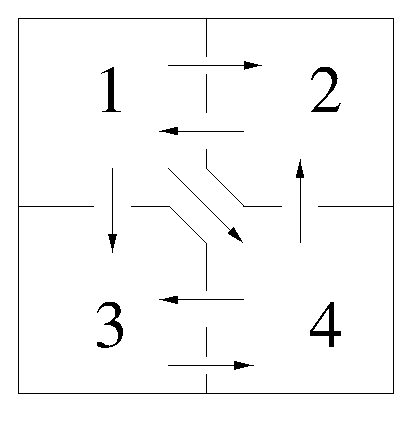
\psfig{file=figures/apart.eps,width=3.2in}}
        \caption{Schematic design of apartment passages.}
        \label{F:apart}
\end{figure}

Suppose that there is a cat in the apartment and that at each hour the cat is
asked to move from the room that it is in to another.  True to form, however,
the cat chooses with equal probability to stay in the room for another hour
or to move through one of the allowed passages.  Suppose that we let $p_{ij}$
be the probability that the cat will move from room~$i$ to room~$j$; in
particular, $p_{ii}$ is the probability that the cat will stay in room~$i$.
For example, when the cat is in room~1, it has four choices  --- it can
stay in room~1 or move to any of the other rooms.  Assuming that each of
these choices is made with equal probability, we see that
\[
p_{11} = \frac{1}{4} \qquad p_{12} = \frac{1}{4} \qquad p_{13} =
\frac{1}{4} \qquad p_{14} = \frac{1}{4}.
\]
It is now straightforward to verify that
\[
p_{21} = \frac{1}{2} \qquad p_{22} = \frac{1}{2} \qquad p_{23} = 0
\qquad p_{24} = 0
\]
\[
p_{31} = 0 \qquad p_{32} = 0 \qquad p_{33} =
\frac{1}{2} \qquad p_{34} = \frac{1}{2}
\]
\[
p_{41} = 0 \qquad p_{42} = \frac{1}{3} \qquad p_{43} =
\frac{1}{3} \qquad p_{44} = \frac{1}{3}.
\]

Putting these probabilities together yields the
{\em transition matrix}\index{matrix!transition}:
\begin{equation*} \label{E:Pexamp}
P = \left(\begin{array}{cccc}
\frac{1}{4} & \frac{1}{4} & \frac{1}{4} & \frac{1}{4} \\
\half & \half & 0 & 0 \\
 0 & 0 & \half & \half\\
0 & \frac{1}{3} & \frac{1}{3} & \frac{1}{3}
\end{array}\right)
\end{equation*}
This transition matrix has the properties that all entries are nonnegative
and that the entries in each row sum to $1$.

\subsubsection*{Three Basic Questions}

Using the transition matrix $P$, we discuss the answers to three questions:
\begin{enumerate}
\item[(A)] What is the probability that a cat starting in room~$i$ will
be in room~$j$ after exactly $k$ steps?  We call the movement that occurs
after each hour a {\em step\/}.
\item[(B)] Suppose that we put 100 cats in the apartment with some initial
distribution of cats in each room.  What will the distribution of cats
look like after a large number of steps?
\item[(C)] Suppose that a cat is initially in room~$i$ and takes a large
number of steps.  For how many of those steps will the cat be expected to
be in room~$j$?
\end{enumerate}

\subsubsection*{A Discussion of Question (A)}

We begin to answer Question (A) by determining the probability that the
cat moves from room~1 to room~4 in two steps.  We denote this probability
by $p_{14}^{(2)}$ and compute
\begin{equation} \label{E:prob14}
p_{14}^{(2)} = p_{11}p_{14} + p_{12}p_{24} + p_{13}p_{34} + p_{14}p_{44};
\end{equation}
that is, the probability is the sum of the probabilities that the cat will
move from room~$1$ to each room~$i$ and then from room~$i$ to room~4.  In
this case the answer is:
\[
p_{14}^{(2)} = \frac{1}{4}\times\frac{1}{4} + \frac{1}{4}\times0 +
\frac{1}{4}\times\frac{1}{2} + \frac{1}{4}\times\frac{1}{3} =
\frac{13}{48} \approx 0.27\;.
\]
It follows from \Ref{E:prob14} and the definition of matrix multiplication
that $p_{14}^{(2)}$ is just the $(1,4)^{th}$ entry in the matrix $P^2$.  An
induction argument shows that the probability of the cat moving from
room~$i$ to room~$j$ in $k$ steps is precisely the $(i,j)^{th}$ entry in the
matrix $P^k$ --- which answers Question (A).  In particular, we can answer the
question: What is the probability that the cat will move from room~4 to room~3
in four steps?  Using \Matlab the answer is given by typing {\tt e4\_10\_1} to
recall the matrix $P$ and then typing
\begin{verbatim}
P4 = P^4;
P4(4,3)
\end{verbatim}
obtaining
\begin{verbatim}
ans =
    0.2728
\end{verbatim}

\subsubsection*{A Discussion of Question (B)}

We answer Question (B) in two parts: first we compute a formula for
determining the number of cats that are expected to be in room~$i$ after $k$
steps, and second we explore that formula numerically for large $k$.  We
begin by supposing that 100 cats are distributed in the rooms according to
the initial vector $V_0=(v_1,v_2,v_3,v_4)^t$; that is, the number of cats
initially in room~$i$ is $v_i$.  Next, we denote the number of cats that are
expected to be in room~$i$ after $k$ steps by $v_i^{(k)}$.  For example, we
determine how many cats we expect to be in room~2 after one step.  That
number is:
\begin{equation} \label{E:probt2}
v_2^{(1)}=p_{12}v_1 + p_{22}v_2 + p_{32}v_3 + p_{42}v_4;
\end{equation}
that is, $v_2^{(1)}$ is the sum of the proportion of cats in each room~$i$
that are expected to migrate to room~2 in one step.  In this case, the answer
is:
\[
\frac{1}{4}v_1 + \frac{1}{2}v_2 + \frac{1}{3}v_4.
\]
It now follows from \Ref{E:probt2}, the definition of the transpose of a
matrix, and the definition of matrix multiplication that $v_2^{(1)}$ is
the $2^{nd}$ entry in the vector $P^tV_0$.  Indeed, it follows by induction
that $v_i^{(k)}$ is the $i^{th}$ entry in the vector $(P^t)^kV_0$ which
answers the first part of Question (B).

We may rephrase the second part of Question (B) as follows.  Let
\[
V_k = (v_1^{k},v_2^{k},v_3^{k},v_4^{k})^t = (P^t)^kV_0.
\]
Question (B) actually asks: What will the vector $V_k$ look like for
large $k$.  To answer that question we need some results about matrices
like the matrix $P$ in \Ref{E:Pexamp}.  But first we explore the answer to
this question numerically using \Matlabp.

Suppose, for example, that the initial vector is
\begin{equation*}
V_0 =\left(\begin{array}{c} 2 \\ 43 \\ 21 \\ 34 \end{array}\right).
\end{equation*}
Typing {\tt e4\_10\_1} and {\tt e4\_10\_4} enters the matrix $P$ and the
initial vector $V_0$ into \Matlabp.  To compute $V_{20}$, the distribution
of cats after $20$ steps, type
\begin{verbatim}
Q=P'
V20 = Q^(20)*V0
\end{verbatim}
and obtain
\begin{verbatim}
V20 =
   18.1818
   27.2727
   27.2727
   27.2727
\end{verbatim}
Thus, after rounding to the nearest integer, we expect $27$ cats to be in
each of rooms~2,3 and 4 and 18 cats to be in room~1 after $20$ steps.  In
fact, the vector $V_{20}$
has a remarkable feature.  Compute {\tt Q*V20} in \Matlab and see that
$V_{20} = P^tV_{20}$; that is, $V_{20}$ is, to within four digit numerical
precision, an eigenvector of $P^t$ with eigenvalue equal to $1$.  This
computation was not a numerical accident, as we now describe.  Indeed,
compute $V_{20}$ for several initial distributions $V_0$ of cats and see that
the answer will always be the same --- up to four digit accuracy.

\subsubsection*{A Discussion of Question (C)}

Suppose there is just one cat in the apartment; and we ask how many times that
cat is expected to visit room~3 in $100$ steps.  Suppose the cat starts in
room~1; then the initial distribution of cats is one cat in room~1 and zero
cats in any of the other rooms.  So $V_0=e_1$.  In our discussion of
Question (B) we saw that the $3^{rd}$ entry in $(P^t)^kV_0$ gives the
probability $c_k$ that the cat will be in room~3 after $k$ steps.

In the extreme, suppose that the probability that the cat will be in room~3 is
$1$ for each step $k$.  Then the fraction of the time that the cat is in room~3
is
\[
(1 + 1 + \cdots + 1)/100 = 1.
\]
In general, the fraction of the time $f$ that the cat will be in room~3
during a span of $100$ steps is
\[
f = \frac{1}{100}(c_1 + c_2 +\cdots + c_{100}).
\]
Since $c_k = (P^t)^kV_0$, we see that
\begin{equation}  \label{E:f}
f = \frac{1}{100}(P^tV_0 + (P^t)^2V_0 + \cdots + (P^t)^{100}V_0).
\end{equation}

So, to answer Question (C), we need a way to sum the expression for $f$
in \Ref{E:f}, at least approximately.  This is not an easy task --- though
the answer itself is easy to explain.  Let $V$ be the eigenvector of $P^t$
with eigenvalue $1$ such that the sum of the entries in $V$ is $1$.  The
answer is: $f$ is approximately equal to $V$.  See Theorem~\ref{T:ergodic}
for a more precise statement.

In our previous calculations the vector $V_{20}$ was seen to be (approximately)
an eigenvector of $P^t$ with eigenvalue $1$.  Moreover the sum of the entries
in $V_{20}$ is precisely $100$.  Therefore, we normalize $V_{20}$ to get $V$
by setting
\[
V =\frac{1}{100}V_{20}.
\]
So, the fraction of time that the cat spends in room~3 is $f\approx 0.2727$.
Indeed, we expect the cat to spend approximately $27\%$ of its time in rooms
2,3,4 and about $18\%$ of its time in room~1.

\subsection*{Markov Matrices}

We now abstract the salient properties of our cat example.  A
{\em Markov chain\/}\index{Markov chain} is a system with a
finite number of states labeled
$1$,\dots,$n$ along with probabilities $p_{ij}$ of moving from site $i$ to
site $j$ in a single step.  The Markov assumption is that these probabilities
depend only on the site that you are in and not on how you got there.  In our
example, we assumed that the probability of the cat moving from say room~2 to
room~4 did not depend on how the cat got to room~2 in the first place.

We make a second assumption: there is a $k$ such that it is possible to move
from any site $i$ to any site $j$ in exactly $k$ steps.  This assumption is
{\em not\/} valid for general Markov chains, though it is valid for the cat
example, since it is possible to move from any room to any other room in that
example in exactly three steps.  (It takes a minimum of three steps to get
from room~3 to room~1 in the cat example.)  To simplify our discussion we
include this assumption in our definition of a Markov chain.

\begin{Def}  \label{D:Markov}
{\em Markov matrices\/}\index{matrix!Markov} are square matrices
$P$ such that
\begin{enumerate}
\item[(a)]  all entries in $P$ are nonnegative,
\item[(b)]  the entries in each row of $P$ sum to $1$, and
\item[(c)]  there is a positive integer $k$ such that all of the entries
	in $P^k$ are positive.
\end{enumerate}
\end{Def}

It is straightforward to verify that parts (a) and (b) in the definition of
Markov matrices are satisfied by the transition matrix
\[
P = \left(\begin{array}{ccc} p_{11} & \cdots & p_{1n} \\
	\vdots & \vdots & \vdots \\ p_{n1} & \cdots & p_{nn}
\end{array}\right)
\]
of a Markov chain.  To verify part (c) requires further discussion.

\begin{prop}   \label{T:Markoveasy}
Let $P$ be a transition matrix\index{matrix!transition} for a
Markov chain\index{Markov chain}.
\begin{enumerate}
\item[(a)]  The probability of moving from site $i$ to site $j$ in exactly
$k$ steps is the $(i,j)^{th}$ entry in the matrix $P^k$.
\item[(b)]  The expected number of individuals at site $i$ after exactly $k$
steps is the $i^{th}$ entry in the vector $V_k\equiv (P^t)^kV_0$.
\item[(c)]  $P$ is a Markov matrix\index{matrix!Markov}.
\end{enumerate}
\end{prop}

\proof Only minor changes in our discussion of the cat example proves parts
(a) and (b) of the proposition.

(c) The assumption that it is possible to move from each site~$i$ to each
site~$j$ in exactly $k$ steps means that the $(i,j)^{th}$ entry of $P^k$ is
positive.  For that $k$, all of the entries of $P^k$ are positive.  In the
cat example, all entries of $P^3$ are positive.  \qed

Proposition~\ref{T:Markoveasy} gives the answer to Question (A) and the first
part of Question (B) for general Markov chains.

Let $v_i^{(0)}\ge 0$ be the number of individuals initially at site $i$, and
let $V_0=(v_1^{(0)},\ldots,v_n^{(0)})^t$.  The total number of individuals
in the initial population is:
\[
\#(V_0) = v_1^{(0)} + \cdots + v_n^{(0)}.
\]

\begin{thm}  \label{T:Markov}
Let $P$ be a Markov matrix\index{matrix!Markov}.  Then
\begin{enumerate}
\item[(a)]  $\#(V_k)=\#(V_0)$; that is, the number of individuals after $k$
time steps is the same as the initial number.
\item[(b)]  $\dps V = \lim_{k\to\infty}V_k$ exists and $\#(V)=\#(V_0)$.
\item[(c)]  $V$ is an eigenvector of $P^t$ with eigenvalue equal to $1$.
\end{enumerate}
\end{thm}

\proof  (a) By induction it is sufficient to show that $\#(V_1)=\#(V_0)$.  We
do
this by calculating from $V_1 = P^tV_0$ that
\begin{eqnarray*}
\#(V_1) & = & v_1^{(1)} + \cdots + v_n^{(1)}\\
& = & (p_{11}v_1^{(0)} + \cdots + p_{n1}v_n^{(0)}) + \cdots +
	(p_{1n}v_1^{(0)} + \cdots + p_{nn}v_n^{(0)}) \\
& = & (p_{11}+ \cdots + p_{1n})v_1^{(0)}  + \cdots +
	(p_{n1} + \cdots + p_{nn})v_n^{(0)} \\
& = & v_1^{(0)}  + \cdots + v_n^{(0)}
\end{eqnarray*}
since the entries in each row of $P$ sum to $1$.  Thus $\#(V_1)=\#(V_0)$, as
claimed.

(b)	The hard part of this theorem is proving that the limiting vector $V$
exists; we give a proof of this fact in Chapter~\ref{C:HDeigenvalues},
Theorem~\ref{T:convergetoeig}.  Once $V$ exists it follows directly from (a)
that $\#(V)=\#(V_0)$.

(c)   	Just calculate that
\[
P^tV = P^t(\lim_{k\to\infty}V_k) = P^t(\lim_{k\to\infty}(P^t)^kV_0)
= \lim_{k\to\infty}(P^t)^{k+1}V_0 = \lim_{k\to\infty}(P^t)^kV_0 = V,
\]
which proves (c).   \qed

Theorem~\ref{T:Markov}(b) gives the answer to the second part of Question (B)
for general Markov chains.  Next we discuss Question (C).

\begin{thm} \label{T:ergodic}
Let $P$ be a Markov matrix\index{matrix!Markov}.
Let $V$ be the eigenvector of $P^t$ with
eigenvalue $1$ and $\#(V)=1$.  Then after a large number of steps $N$ the
expected number of times an individual will visit site~$i$ is $Nv_i$ where
$v_i$ is the $i^{th}$ entry in $V$.
\end{thm}

\noindent {\bf Sketch of proof:}  In our discussion of Question (C) for the
cat example, we explained why the fraction $f_N$ of time that an individual
will visit site~$j$ when starting initially at site~$i$ is the $j^{th}$ entry
in the sum
\[
f_N = \frac{1}{N}(P^t + (P^t)^2 + \cdots + (P^t)^N)e_i.
\]
See \Ref{E:f}.  The proof of this theorem involves being able to calculate
the limit of $f_N$ as $N\to\infty$.  There are two main ideas.  First, the
limit of the matrix $(P^t)^N$ exists as $N$ approaches infinity --- call that
limit $Q$.  Moreover, $Q$ is a matrix all of whose columns equal $V$.
Second, for large $N$, the sum
\[
P^t + (P^t)^2 + \cdots + (P^t)^N \approx Q + Q + \cdots + Q = NQ,
\]
so that the limit of the $f_N$ is $Qe_i=V$.

The verification of these statements is beyond the scope of this text.
For those interested, the idea of the proof of the second part is roughly the
following.  Fix $k$ large enough so that $(P^t)^k$ is close to $Q$.  Then when
$N$ is large, much larger than $k$, the sum of the first $k$ terms in the
series is nearly zero.  \qed


Theorem~\ref{T:ergodic} gives the answer to Question (C) for a general Markov
chain.  It follows from Theorem~\ref{T:ergodic} that for Markov chains the
amount of time that an individual spends in room~$i$ is independent of the
individual's initial room --- at least after a large number of steps.

A complete proof of this theorem relies on a result known as the {\em ergodic
theorem}.
Roughly speaking, the ergodic theorem relates space averages
with time averages.   To see how this point is relevant, note that Question (B)
deals with the issue of how a large number of individuals will be distributed
in space after a large number of steps, while Question (C) deals with the
issue of how the path of a single individual will be distributed in time after
a large number of steps.

\subsubsection*{An Example of Umbrellas}

This example focuses on the utility of answering Question (C) and reinforces
the fact that results in Theorem~\ref{T:Markov} have the second
interpretation given in Theorem~\ref{T:ergodic}.

Consider the problem of a man with four umbrellas.  If it is raining in the
morning when the man is about to leave for his office, then the man takes an
umbrella from home to office, assuming that he has an umbrella at home.  If it
is raining in the afternoon, then the man takes an umbrella from office to
home, assuming that he has an umbrella in his office.  Suppose that the
probability that it will rain in the morning is $p=0.2$ and the probability
that it will rain in the afternoon is $q=0.3$, and these probabilities are
independent.  What percentage of days will the man get wet going from home
to office; that is, what percentage of the days will the man be at home on a
rainy morning with all of his umbrellas at the office?

There are five states in the system depending on the number of umbrellas that
are at home.  Let $s_i$ where $0\leq i\leq 4$ be the state with $i$ umbrellas
at home and $4-i$ umbrellas at work.  For example, $s_2$ is the state of
having two umbrellas at home and two at the office.  Let $P$ be the
$5\times 5$ transition matrix of state changes from morning to afternoon and
$Q$ be the $5\times 5$ transition matrix of state changes from afternoon to
morning.  For example, the probability $p_{23}$ of moving from site $s_2$ to
site $s_3$ is $0$, since it is not possible to have more umbrellas at home
after going to work in the morning.  The probability $q_{23}=q$, since the
number of umbrellas at home will increase by one only if it is raining in the
afternoon.  The transition probabilities between all states are given in the
following transition matrices:
\[
P = \left(\begin{array}{ccccc} 1 & 0 & 0 & 0 & 0 \\
  p & 1-p & 0 & 0 & 0 \\ 0 & p & 1-p & 0 & 0 \\ 0 & 0 & p & 1-p & 0 \\
 0 & 0 & 0 & p & 1-p \end{array}\right); \quad
Q = \left(\begin{array}{ccccc} 1-q & q & 0 & 0 & 0 \\
  0 & 1-q & q & 0 & 0 \\ 0 & 0 & 1-q & q & 0 \\ 0 & 0 & 0 & 1-q & q \\
 0 & 0 & 0 & 0 & 1 \end{array}\right)
\]
Specifically,
\begin{equation*}
P =
\left(\begin{array}{ccccc} 1 & 0 & 0 & 0 & 0 \\
  0.2 & 0.8 & 0 & 0 & 0 \\ 0 & 0.2 & 0.8 & 0 & 0 \\ 0 & 0 & 0.2 & 0.8 & 0 \\
 0 & 0 & 0 & 0.2 & 0.8 \end{array}\right) \AND
Q =
\left(\begin{array}{ccccc} 0.7 & 0.3 & 0 & 0 & 0 \\
  0 & 0.7 & 0.3 & 0 & 0 \\ 0 & 0 & 0.7 & 0.3 & 0 \\ 0 & 0 & 0 & 0.7 & 0.3 \\
 0 & 0 & 0 & 0 & 1 \end{array}\right)
\end{equation*}

The transition matrix\index{matrix!transition} $M$ from
moving from state $s_i$ on one morning to
state $s_j$ the next morning is just $M=PQ$.  We can compute this matrix
using \Matlab by typing
\begin{verbatim}
e4_10_6
M = P*Q
\end{verbatim}
obtaining
\begin{verbatim}
M =
    0.7000    0.3000         0         0         0
    0.1400    0.6200    0.2400         0         0
         0    0.1400    0.6200    0.2400         0
         0         0    0.1400    0.6200    0.2400
         0         0         0    0.1400    0.8600
\end{verbatim}
It is easy to check using \Matlab that all entries in the matrix $M^4$ are
nonzero.  So $M$ is a Markov matrix\index{matrix!Markov} and we can use
Theorem~\ref{T:ergodic}
to find the limiting distribution of states.  Start with some initial
condition like $V_0=(0,0,1,0,0)^t$ corresponding to the state in which two
umbrellas are at home and two at the office.  Then compute the vectors
$V_k=(M^t)^kV_0$ until arriving at an eigenvector of $M^t$ with eigenvalue 1.
For example, $V_{70}$ is computed by typing \verb+V70 = M'^(70)*V0+ and
obtaining
\begin{verbatim}
V70 =
    0.0419
    0.0898
    0.1537
    0.2633
    0.4512
\end{verbatim}
We interpret $V\approx V_{70}$ in the following way.  Since $v_1$ is
approximately $.042$, it follows that for approximately $4.2\%$ of all steps 
the umbrellas are in state $s_0$.  That is, approximately $4.2\%$ of all days 
there are no umbrellas at home.  The probability that it will rain in the 
morning on one of those days is $0.2$.  Therefore, the probability of being 
at home in the morning when it is raining without any umbrellas is 
approximately $0.008$.





\EXER

\TEXER

\begin{exercise} \label{c4.10.1}
Let $P$ be a Markov matrix and let $w=(1,\ldots,1)^t$.  Show that
the vector $w$ is an eigenvector of $P$ with eigenvalue $1$.
\end{exercise}

\noindent In Exercises~\ref{c4.10.2a} -- \ref{c4.10.2c} which of the
matrices are Markov matrices, and why?
\begin{exercise} \label{c4.10.2a}
$P = \mattwo{0.8}{0.2}{0.2}{0.8}$.
\end{exercise}
\begin{exercise} \label{c4.10.2b}
$Q = \mattwo{0.8}{0.2}{0}{1}$.
\end{exercise}
\begin{exercise} \label{c4.10.2c}
$R = \mattwo{0.8}{0.2}{-0.2}{1.2}$.
\end{exercise}

\begin{exercise} \label{c4.10.3}
The state diagram of a Markov chain is given in Figure~\ref{F:Mchain}.
Assume that each arrow leaving a state has equal probability of being chosen.
Find the transition matrix for this chain.
\end{exercise}
\begin{figure}[htb]
        \centerline{%
        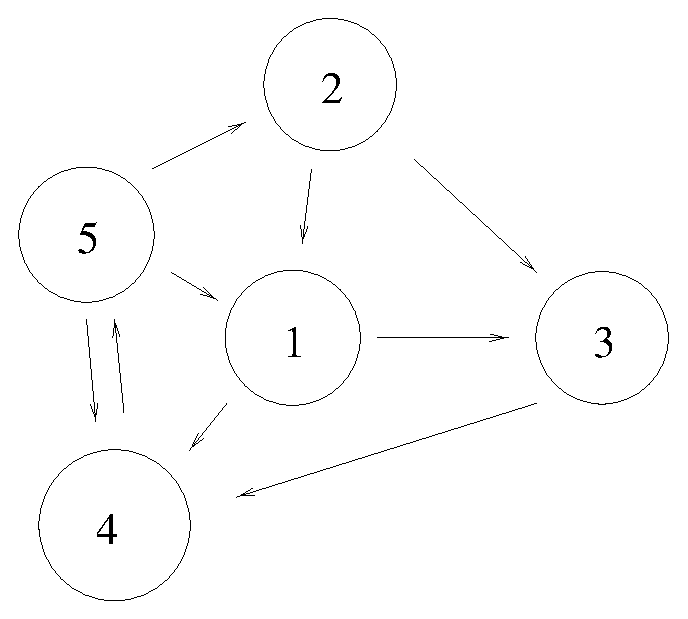
\psfig{file=figures/Mchain.eps,width=3.0in}}
        \caption{State diagram of a Markov chain.}
        \label{F:Mchain}
\end{figure}


\begin{exercise} \label{c4.10.4}
Suppose that $P$ and $Q$ are each $n\times n$ matrices whose rows sum to $1$.
Show that $PQ$ is also an $n\times n$ matrix whose rows sum to $1$.
\end{exercise}



\CEXER

\begin{exercise} \label{c4.10.5}
Suppose the apartment in Figure~\ref{F:apart} is populated by dogs rather than
cats.  Suppose that dogs will actually move when told; that is, at each step
a dog will move from the room that he occupies to another room.
\begin{itemize}
\item[(a)]  Calculate the transition matrix {\tt PDOG} for this Markov chain
and verify that {\tt PDOG} is a Markov matrix.
\item[(b)]  Find the probability that a dog starting in room~2 will end up in
room~3 after $5$ steps.
\item[(c)]  Find the probability that a dog starting in room~3 will end up in
room~1 after $4$ steps.  Explain why your answer is correct without using
\Matlabp.
\item[(d)]  Suppose that the initial population consists of 100 dogs.  After
a large number of steps what will be the distribution of the dogs in the four
rooms.
\end{itemize}
\end{exercise}

\begin{exercise} \label{c4.10.6}
A truck rental company has locations in three cities A, B and C.
Statistically, the company knows that the trucks rented at one location will
be returned in one week to the three locations in the following proportions.
\begin{center}
\begin{tabular}{|c||c|c|c|}
\hline
Rental Location &  Returned to A & Returned to B & Returned to C\\
\hline
A  & 75\% & 10\%  & 15\% \\
\hline
B & 5\% & 85\% & 10\% \\
\hline
C & 20\% & 20\% & 60\%\\
\hline
\end{tabular}
\end{center}
Suppose that the company has 250 trucks.  How should the company distribute
the trucks so that the number of trucks available at each location remains
approximately constant from one week to the next?
\end{exercise}

\begin{exercise} \label{c4.10.7}
Let
\begin{equation*}
P = \left(\begin{array}{ccccc}
 0.10 & 0.20 & 0.30 & 0.15 & 0.25\\
 0.05 & 0.35 & 0.10 & 0.40 & 0.10\\
   0  &   0  & 0.35 & 0.55 & 0.10\\
 0.25 & 0.25 & 0.25 & 0.25 &   0\\
 0.33 & 0.32 &   0  &   0  & 0.35
\end{array}\right)
\end{equation*}
be the transition matrix of a Markov chain.
\begin{itemize}
\item[(a)]  What is the probability that an individual at site~2 will move to
site~5 in three steps?
\item[(b)]  What is the probability that an individual at site~4 will move to
site~1 in seven steps?
\item[(c)]  Suppose that 100 individuals are initially uniformly distributed
at the five sites.  How will the individuals be distributed after four steps?
\item[(d)]  Find an eigenvector of $P^t$ with eigenvalue $1$.
\end{itemize}
\end{exercise}

\begin{exercise} \label{c4.10.8}
Suppose that the probability that it will rain in the morning in $p=0.3$ and
the probability that it will rain in the afternoon is $q=0.25$.  In the man
with umbrellas example, what is the probability that the man will be at home
with no umbrellas while it is raining?
\end{exercise}

\begin{exercise} \label{c4.10.9}
Suppose that the original man in the text with umbrellas has only three
umbrellas instead of four.  What is the probability that on a given day he
will get wet going to work?
\end{exercise}



